\documentclass{jfp}

\usepackage[utf8]{inputenc}
% \usepackage{amsmath}
% \usepackage{amssymb}

\bibliographystyle{JFPlike}


% %% Some recommended packages.
% \usepackage{booktabs}   %% For formal tables:
%                         %% http://ctan.org/pkg/booktabs
\usepackage{subcaption} %% For complex figures with subfigures/subcaptions
                        %% http://ctan.org/pkg/subcaption
\usepackage{wrapfig}

\usepackage{placeins}

\usepackage[disable]{todonotes}

\usepackage{ifthen}
\usepackage{pgf}
\usepackage{ulem}
\usepackage{tikz}
\usepackage{tikzpeople}
\usetikzlibrary{backgrounds}
\usetikzlibrary{fit}
\usetikzlibrary{calc}
\usetikzlibrary{positioning}
\usetikzlibrary{patterns}
\usetikzlibrary{decorations.pathreplacing}
\usetikzlibrary{arrows,shapes}
\usepackage{amssymb}

% Active adversary
\newcommand{\actadv}[4][]{
  \ifthenelse{\equal{#1}{}}{
    \draw[fill=white] #2 rectangle #3 node[pos=.5] {};
    \draw ($#2 + (2.25,1.5)$) node[devil,mirrored,minimum size=1cm] {};
    \draw[fill=white, fill opacity=0.5] #2 rectangle #3 node[pos=.5] {};
    \draw #2 rectangle #3 node[pos=.5,align=center] {\footnotesize #4};
  }{
    \onlyenv<#1>
    \draw[fill=white] #2 rectangle #3 node[pos=.5] {};
    \draw ($#2 + (3,1.5)$) node[devil,mirrored,minimum size=1cm] {};
    \draw[fill=white, fill opacity=0.5] #2 rectangle #3 node[pos=.5] {};
    \draw #2 rectangle #3 node[pos=.5] {\footnotesize #4};
    \endonlyenv
  }
}

% Inactive adversary
\newcommand{\inactadv}[4][]{
  \ifthenelse{\equal{#1}{}}{
    \draw[fill=white] #2 rectangle #3 node[pos=.5] {};
    \draw ($#2 + (2.25,1.5)$) node[devil,mirrored,minimum size=1cm] {};
    \draw[fill=white, fill opacity=0.4] #2 rectangle #3 node[pos=.5] {};
    \draw[fill=gray, fill opacity=0.5] #2 rectangle #3 node[pos=.5] {};
    \draw #2 rectangle #3 node[pos=.5] {\footnotesize #4};
  }{
    \onlyenv<#1>
    \draw[fill=white] #2 rectangle #3 node[pos=.5] {};
    \draw ($#2 + (3,1.5)$) node[devil,mirrored,minimum size=1cm] {};
    \draw[fill=white, fill opacity=0.4] #2 rectangle #3 node[pos=.5] {};
    \draw[fill=gray, fill opacity=0.5] #2 rectangle #3 node[pos=.5] {};
    \draw #2 rectangle #3 node[pos=.5] {\footnotesize #4};
    \endonlyenv
  }
}

% Active stack frame
\newcommand{\actsf}[4][]{
  \ifthenelse{\equal{#1}{}}{
    \draw[fill=white] #2 rectangle #3 node[pos=.5] {\footnotesize #4};
  }{
   \draw<#1>[fill=white] #2 rectangle #3 node[pos=.5] {#4};
 }
}

% Inactive stack frame
\newcommand{\inactsf}[4][]{
  \ifthenelse{\equal{#1}{}}{
    \draw[fill=white] #2 rectangle #3 node[pos=.5] {};
    \draw[fill=gray, fill opacity=0.5] #2 rectangle #3 node[pos=.5] {};
    \draw #2 rectangle #3 node[pos=.5] {\footnotesize #4};
  }{
    \draw<#1>[fill=white] #2 rectangle #3 node[pos=.5] {};
    \draw<#1>[fill=gray, fill opacity=0.5] #2 rectangle #3 node[pos=.5] {};
    \draw<#1> #2 rectangle #3 node[pos=.5] {\footnotesize #4};
  }
}

\newcommand{\capbrace}[3][sp1]{
  \draw [decorate,decoration={brace,amplitude=10pt,mirror,raise=4pt},yshift=0pt]
  #2 -- #3 node[draw=black] (#1) [black,midway,xshift=0.8cm] {};

}

\newcommand{\stdstackstart}{
  \scope
    \clip (-.1,-.1) rectangle (4.6,11.1);
    \fill[fill=white] (0,0) rectangle (4.5,11);
    \draw (0,0) -- (0,11);
    \draw (4.5,0) -- (4.5,11);
    \draw[fill=gray!50] (0,-.5) rectangle (4.5,2)
    node[pos=.5,color=black,align=center,yshift=0.1cm] {\footnotesize Higher
      stack\\\footnotesize frames...};
  \endscope
  % \draw[->] (-2,0) -- node[midway,sloped,above] {stack grows upward} (-2,15);
  \draw (-1.5,0) node {};
  \draw (-1.5,15) node {};
}


% stolen from https://tex.stackexchange.com/questions/14225/is-there-the-easiest-way-to-toggle-show-hide-navigational-grids-in-tikz/14230
\makeatletter
\newif\if@showgrid@grid
\newif\if@showgrid@left
\newif\if@showgrid@right
\newif\if@showgrid@below
\newif\if@showgrid@above
\tikzset{%
    every show grid/.style={},
    show grid/.style={execute at end picture={\@showgrid{grid=true,#1}}},%
    show grid/.default={true},
    show grid/.cd,
    labels/.style={font={\sffamily\small},help lines},
    xlabels/.style={},
    ylabels/.style={},
    keep bb/.code={\useasboundingbox (current bounding box.south west) rectangle (current bounding box.north west);},
    true/.style={left,below},
    false/.style={left=false,right=false,above=false,below=false,grid=false},
    none/.style={left=false,right=false,above=false,below=false},
    all/.style={left=true,right=true,above=true,below=true},
    grid/.is if=@showgrid@grid,
    left/.is if=@showgrid@left,
    right/.is if=@showgrid@right,
    below/.is if=@showgrid@below,
    above/.is if=@showgrid@above,
    false,
}

\def\@showgrid#1{%
    \begin{scope}[every show grid,show grid/.cd,#1]
    \if@showgrid@grid
    \begin{pgfonlayer}{background}
    \draw [help lines]
        (current bounding box.south west) grid
        (current bounding box.north east);
%
    \pgfpointxy{1}{1}%
    \edef\xs{\the\pgf@x}%
    \edef\ys{\the\pgf@y}%
    \pgfpointanchor{current bounding box}{south west}
    \edef\xa{\the\pgf@x}%
    \edef\ya{\the\pgf@y}%
    \pgfpointanchor{current bounding box}{north east}
    \edef\xb{\the\pgf@x}%
    \edef\yb{\the\pgf@y}%
    \pgfmathtruncatemacro\xbeg{ceil(\xa/\xs)}
    \pgfmathtruncatemacro\xend{floor(\xb/\xs)}
    \if@showgrid@below
    \foreach \X in {\xbeg,...,\xend} {
        \node [below,show grid/labels,show grid/xlabels] at (\X,\ya) {\X};
    }
    \fi
    \if@showgrid@above
    \foreach \X in {\xbeg,...,\xend} {
        \node [above,show grid/labels,show grid/xlabels] at (\X,\yb) {\X};
    }
    \fi
    \pgfmathtruncatemacro\ybeg{ceil(\ya/\ys)}
    \pgfmathtruncatemacro\yend{floor(\yb/\ys)}
    \if@showgrid@left
    \foreach \Y in {\ybeg,...,\yend} {
        \node [left,show grid/labels,show grid/ylabels] at (\xa,\Y) {\Y};
    }
    \fi
    \if@showgrid@right
    \foreach \Y in {\ybeg,...,\yend} {
        \node [right,show grid/labels,show grid/ylabels] at (\xb,\Y) {\Y};
    }
    \fi
    \end{pgfonlayer}
    \fi
    \end{scope}
}
\makeatother


 	
%%% Local Variables:
%%% TeX-master: "paper"
%%% End:
\usetikzlibrary{fit}
\makeatletter
\tikzset{
  fitting node/.style={
    inner sep=0pt,
    fill=none,
    draw=none,
    reset transform,
    fit={(\pgf@pathminx,\pgf@pathminy) (\pgf@pathmaxx,\pgf@pathmaxy)}
  },
  reset transform/.code={\pgftransformreset}
}
\makeatother

% prevent a compilation failure with JFP.
\undef{\base}
% Math packages
\usepackage{amsmath,amsfonts,amssymb,amsthm}
\usepackage{mathrsfs}
\usepackage{thmtools}
\usepackage{array}
\usepackage{cleveref}
\usepackage{stmaryrd}
\usepackage{mathpartir}


% Command control packages
\usepackage{ifthen}
\usepackage{ifpdf}

% Listings
\usepackage{listings}
\lstset{
  basicstyle=\ttfamily,
  columns=fullflexible,
  keepspaces=true,
  mathescape
}


% Tikz
\usepackage{tikz}

%%% Comments
% Comments
\newcommand\lau[1]{{\color{purple} \sf \footnotesize {LS: #1}}\\}
\newcommand\dominique[1]{{\color{purple} \sf \footnotesize {DD: #1}}\\}
\newcommand\lars[1]{{\color{purple} \sf \footnotesize {LB: #1}}\\}

%%% Math environments
\declaretheorem[numbered=yes,name=Lemma,qed=$\blacksquare$]{lemma}
\declaretheorem[numbered=yes,name=Theorem,qed=$\blacksquare$]{theorem}
\declaretheorem[numbered=yes,name=Definition,qed=$\blacksquare$]{definition}
\declaretheorem[numbered=yes,name=Specification,qed=$\blacksquare$]{specification}


%%% Math notation
\newcommand{\defeq}{\stackrel{\textit{\tiny{def}}}{=}}
\newcommand{\defbnf}{::=}
\newcommand{\sem}[1]{\left\llbracket #1 \right\rrbracket}
\newcommand{\ssem}[2][\Phi]{\sem{#2}_{\mathrm{src}}(#1)}
\newcommand{\tsem}[2][\Phi]{\sem{#2}_{\mathrm{trg}}(#1)}
\newcommand{\dom}{\mathrm{dom}}
\newcommand{\powerset}[1]{\mathcal{P}(#1)}

\newcommand{\npair}[2][n]{\left(#1,#2\right)}

\newcommand{\nsubeq}[1][n]{\overset{#1}{\subseteq}}
\newcommand{\nsupeq}[1][n]{\overset{#1}{\supseteq}}
\newcommand{\nequal}[1][n]{\overset{#1}{=}}

% Function arrows
\newcommand{\fun}{\rightarrow}
\newcommand{\parfun}{\rightharpoonup}
\newcommand{\monnefun}{\xrightarrow{\textit{\tiny{mon, ne}}}}



% Text
\newcommand{\tand}{\text{ and }}
\newcommand{\tor}{\text{ or }}
\newcommand{\totherwise}{\text{otherwise }}

% Equivalences
\newcommand{\sconeq}{\mathrel{\src{\approx_{\mathrm{ctx}}}}}
\newcommand{\tconeq}{\mathrel{\approx_{\mathrm{ctx}}}}

%%% Logical Relation notation
\newcommand{\typesetlr}[1]{\mathcal{#1}}
\newcommand{\lre}{\typesetlr{E}}
\newcommand{\lrexj}{\typesetlr{E}_{\var{xjmp}}}
\newcommand{\lrk}{\typesetlr{K}}
\newcommand{\lrr}{\typesetlr{R}}
\newcommand{\lro}{\typesetlr{O}}
\newcommand{\lrv}{\typesetlr{V}}
\newcommand{\lrp}{\typesetlr{P}}
\newcommand{\lrm}{\typesetlr{M}}

\newcommand{\stpair}[3][]{
\ifthenelse{\equal{#1}{}}
{\left(\src{#2_S},#3_T\right)}
{\left(\src{#2},#3\right)}}


\newcommand{\memSat}[3][n]{#2 :_{#1}#3}

\newcommand{\World}{\mathrm{World}}
\newcommand{\RegionName}{\mathrm{RegionName}}
\newcommand{\Region}{\mathrm{Region}}
\newcommand{\spatial}{\mathrm{spatial}}
\newcommand{\spatialo}{\mathrm{spatial\_owned}}
\newcommand{\pure}{\mathrm{pure}}
\newcommand{\revoked}{\mathrm{revoked}}
\newcommand{\State}{\mathrm{State}}
\newcommand{\Rels}{\mathrm{Rels}}
\newcommand{\UPred}[1]{\mathrm(#1)}

\newcommand{\future}{\sqsupseteq}
\newcommand{\pub}{\mathrm{pub}}
\newcommand{\privft}{\future^{\priv}}
\newcommand{\pubft}{\future^{\pub}}
\newcommand{\monprivnefun}{\xrightarrow[\text{\tiny{$\privft$}}]{\textit{\tiny{mon, ne}}}}
\newcommand{\monpubnefun}{\xrightarrow[\text{\tiny{$\pubft$}}]{\textit{\tiny{mon, ne}}}}

%%% Regions
\newcommand{\stdreg}[2]{\iota^{\mathrm{std},#2}_{#1}}
\newcommand{\stareg}[2][\stpair{\ms}{\ms}]{\iota^{\mathrm{sta},#2}_{#1}}
\newcommand{\spa}{\mathrm{s}}
\newcommand{\spao}{\mathrm{so}}
\newcommand{\pur}{\mathrm{p}}

%%% Instruction formatting
\newcommand{\sourcecolortext}{blue}
\newcommand{\sourcecolor}{\color{blue}}
\newcommand{\src}[1]{{\sourcecolor #1}}
\newcommand{\targetcolortext}{black}
\newcommand{\targetcolor}[1]{\color{black}}
\newcommand{\trg}[1]{{\targetcolor{} #1}}

\newcommand{\zinstr}[1]{\texttt{#1}}
\newcommand{\oneinstr}[2]{
  \ifthenelse{\equal{#2}{}}
  {\zinstr{#1}}
  {\zinstr{#1} \; #2}
}
\newcommand{\twoinstr}[3]{
  \ifthenelse{\equal{#2#3}{}}
  {\zinstr{#1}}
  {\zinstr{#1} \; #2 \; #3}
}
\newcommand{\threeinstr}[4]{
  \ifthenelse{\equal{#2#3#4}{}}
  {\zinstr{#1}}
  {\zinstr{#1} \; #2 \; #3 \; #4}
}

\newcommand{\fourinstr}[5]{
  \ifthenelse{\equal{#2#3#4#5}{}}
  {\zinstr{#1}}
  {\zinstr{#1} \; #2 \; #3 \; #4 \; #5}
}


%%% Source language
% No arguments
\newcommand{\sfail}{\zinstr{\src{fail}}}
\newcommand{\shalt}{\zinstr{\src{halt}}}
\newcommand{\sreturn}{\zinstr{\src{return}}}

% One argument
\newcommand{\sjmp}[1]{\oneinstr{\src{jmp}}{#1}}
\newcommand{\spush}[1]{\oneinstr{\src{push}}{#1}}
\newcommand{\spop}[1]{\oneinstr{\src{pop}}{#1}}

% Two arguments
\newcommand{\sjnz}[2]{\twoinstr{\src{jnz}}{#1}{#2}}
\newcommand{\sisptr}[2]{\twoinstr{\src{gettype}}{#1}{#2}}
\newcommand{\sgeta}[2]{\twoinstr{\src{geta}}{#1}{#2}}
\newcommand{\sgetb}[2]{\twoinstr{\src{getb}}{#1}{#2}}
\newcommand{\sgete}[2]{\twoinstr{\src{gete}}{#1}{#2}}
\newcommand{\sgetp}[2]{\twoinstr{\src{getp}}{#1}{#2}}
%\newcommand{\sgetloc}[2]{\twoinstr{\src{getloc}}{#1}{#2}}
\newcommand{\sgetlin}[2]{\twoinstr{\src{get}}{#1}{#2}}
\newcommand{\smove}[2]{\twoinstr{\src{move}}{#1}{#2}}
\newcommand{\sstore}[2]{\twoinstr{\src{store}}{#1}{#2}}
\newcommand{\sload}[2]{\twoinstr{\src{load}}{#1}{#2}}
\newcommand{\scca}[2]{\twoinstr{\src{cca}}{#1}{#2}}
\newcommand{\ssload}[2]{\twoinstr{\src{sload}}{#1}{#2}}
\newcommand{\sxjmp}[2]{\twoinstr{\src{xjmp}}{#1}{#2}}
\newcommand{\ssetatob}[2]{\twoinstr{\src{seta2b}}{#1}{#2}}
% scall - special two instruction
\newcommand{\scall}[4][]{  
\ifthenelse{\equal{#3#4}{}}
  {\ensuremath{\zinstr{\src{call}}_{#1}^{#2}}}
  {\ensuremath{\zinstr{\src{call}}_{#1}^{#2} \; #3 \; #4}}
}


% Three arguments
\newcommand{\srestrict}[3]{\threeinstr{\src{restrict}}{#1}{#2}{#3}}
\newcommand{\slt}[3]{\threeinstr{\src{lt}}{#1}{#2}{#3}}
\newcommand{\splus}[3]{\threeinstr{\src{plus}}{#1}{#2}{#3}}
\newcommand{\sminus}[3]{\threeinstr{\src{minus}}{#1}{#2}{#3}}
\newcommand{\scseal}[3]{\threeinstr{\src{cseal}}{#1}{#2}{#3}}
\newcommand{\ssplice}[3]{\threeinstr{\src{splice}}{#1}{#2}{#3}}


% Four arguments
%\newcommand{\ssubseg}[4]{\fourinstr{\src{subseg}}{#1}{#2}{#3}{#4}}
\newcommand{\ssplit}[4]{\fourinstr{\src{split}}{#1}{#2}{#3}{#4}}

%%% Target language
% No arguments
\newcommand{\tfail}{\zinstr{\trg{fail}}}
\newcommand{\thalt}{\zinstr{\trg{halt}}}

% One argument
\newcommand{\tjmp}[1]{\oneinstr{\trg{jmp}}{#1}}

% Two arguments
\newcommand{\tjnz}[2]{\twoinstr{\trg{jnz}}{#1}{#2}}
\newcommand{\tisptr}[2]{\twoinstr{\trg{gettype}}{#1}{#2}}
\newcommand{\tgeta}[2]{\twoinstr{\trg{geta}}{#1}{#2}}
\newcommand{\tgetb}[2]{\twoinstr{\trg{getb}}{#1}{#2}}
\newcommand{\tgete}[2]{\twoinstr{\trg{gete}}{#1}{#2}}
\newcommand{\tgetp}[2]{\twoinstr{\trg{getp}}{#1}{#2}}
%\newcommand{\tgetloc}[2]{\twoinstr{\trg{getloc}}{#1}{#2}}
\newcommand{\tgetlin}[2]{\twoinstr{\trg{getl}}{#1}{#2}}
\newcommand{\tmove}[2]{\twoinstr{\trg{move}}{#1}{#2}}
\newcommand{\tstore}[2]{\twoinstr{\trg{store}}{#1}{#2}}
\newcommand{\tload}[2]{\twoinstr{\trg{load}}{#1}{#2}}
\newcommand{\tcca}[2]{\twoinstr{\trg{cca}}{#1}{#2}}
\newcommand{\txjmp}[2]{\twoinstr{\trg{xjmp}}{#1}{#2}}
\newcommand{\tsetatob}[2]{\twoinstr{\trg{seta2b}}{#1}{#2}}

% Three arguments
\newcommand{\tsplice}[3]{\threeinstr{\trg{splice}}{#1}{#2}{#3}}
\newcommand{\trestrict}[3]{\threeinstr{\trg{restrict}}{#1}{#2}{#3}}
\newcommand{\tlt}[3]{\threeinstr{\trg{lt}}{#1}{#2}{#3}}
\newcommand{\tplus}[3]{\threeinstr{\trg{plus}}{#1}{#2}{#3}}
\newcommand{\tminus}[3]{\threeinstr{\trg{minus}}{#1}{#2}{#3}}
\newcommand{\tcseal}[3]{\threeinstr{\trg{cseal}}{#1}{#2}{#3}}

% Four arguments
%\newcommand{\tsubseg}[4]{\fourinstr{\trg{subseg}}{#1}{#2}{#3}{#4}}
\newcommand{\tsplit}[4]{\fourinstr{\trg{split}}{#1}{#2}{#3}{#4}}

%%% Domains
\newcommand{\plaindom}[1]{\mathrm{#1}}

\newcommand{\nats}{\mathbb{N}}
\newcommand{\ints}{\mathbb{Z}}

%%% Updates
\newcommand{\update}[2]{[#1 \mapsto #2]}
\newcommand{\updReg}[2]{\update{\reg.#1}{#2}}
\newcommand{\updPc}[1]{\Phi\updReg{\pcreg}{#1}}

%%% Source dom
\newcommand{\shareddom}[1]{\mathrm{#1}}
\newcommand{\RegName}{\shareddom{RegisterName}}
\newcommand{\Addr}{\shareddom{Addr}}
\newcommand{\Seal}{\shareddom{Seal}}
\newcommand{\Perm}{\shareddom{Perm}}
\newcommand{\Caps}{\shareddom{Cap}}
\newcommand{\SealableCaps}{\shareddom{SealableCap}}
\newcommand{\Word}{\shareddom{Word}}
\newcommand{\Instr}{\shareddom{Instr}}
\newcommand{\Mem}{\shareddom{Memory}}
\newcommand{\Reg}{\shareddom{RegisterFile}}
\newcommand{\Stk}{\shareddom{Stack}}
\newcommand{\Conf}{\shareddom{Conf}}
\newcommand{\ExecConf}{\shareddom{ExecConf}}
%\newcommand{\Global}{\shareddom{Global}}
\newcommand{\Linear}{\shareddom{Linear}}
\newcommand{\MemSeg}{\shareddom{MemorySegment}}
\newcommand{\StkFrame}{\shareddom{StackFrame}}
\newcommand{\Stack}{\shareddom{Stack}}

\newcommand{\scbnf}{\shareddom{sc}}
\newcommand{\cbnf}{\shareddom{c}}
\newcommand{\permbnf}{\shareddom{perm}}
\newcommand{\addrbnf}{\shareddom{a}}
\newcommand{\basebnf}{\shareddom{base}}
\newcommand{\aendbnf}{\shareddom{end}}
\newcommand{\rbnf}{\shareddom{r}}
%\newcommand{\glbnf}{\shareddom{gl}}
\newcommand{\linbnf}{\shareddom{l}}
\newcommand{\sealbasebnf}{\sigma_\shareddom{base}}
\newcommand{\sealendbnf}{\sigma_\shareddom{end}}

\newcommand{\sstk}{\shareddom{stk}}
\newcommand{\smsstk}{\shareddom{ms_{stk}}}
\newcommand{\sstkframe}{\shareddom{frame}}
\newcommand{\sopc}{\shareddom{opc}}
\newcommand{\sastk}{\shareddom{a_{stk}}}
\newcommand{\perm}{\var{perm}}
%\newcommand{\gl}{\var{g}}
\newcommand{\lin}{\var{l}}
\newcommand{\base}{\shareddom{base}}
\newcommand{\aend}{\shareddom{end}}
\newcommand{\addr}{\shareddom{a}}
\newcommand{\scap}{\shareddom{c}}
\newcommand{\sms}{\shareddom{ms}}

\newcommand{\stkptr}[1]{\mathrm{stack\text{-}ptr}(#1)}
\newcommand{\retptr}{\mathrm{ret\text{-}ptr}}
\newcommand{\retptrd}{\mathrm{ret\text{-}ptr\text{-}data}}
\newcommand{\retptrc}{\mathrm{ret\text{-}ptr\text{-}code}}

\newcommand{\seal}[1]{\shareddom{seal}(#1)}
\newcommand{\sealed}[1]{\shareddom{sealed}(#1)}

\newcommand{\failed}{\mathrm{failed}}
% DOMI: defining a macro named ``undefined'' breaks many latex packages.
%       (this is just another way that LaTeX is broken as a programming language)
% \newcommand{\undefined}{\mathrm{undefined}}
\newcommand{\tundefined}{\mathrm{undefined}}
\newcommand{\halted}{\mathrm{halted}}

%%% Target domain
\newcommand{\targetdom}[1]{\mathrm{#1}}
\newcommand{\tRegName}{\targetdom{RegisterName}}

%%% Programs and contexts
\newcommand{\program}{\mathscr{P}}
\newcommand{\context}{\mathscr{C}}

\newcommand{\plug}[2]{#1[#2]}

%%% Operational semantics
\newcommand{\step}{\rightarrow}
\newcommand{\nstep}[1][n]{\step_{#1}}
\newcommand{\steps}{\step^*}
\newcommand{\diverge}{{\Uparrow}}
\newcommand{\term}[1][-]{{\Downarrow_{#1}}}

%%% Variables
\newcommand{\var}[1]{\mathit{#1}}
\newcommand{\rn}{\var{rn}}
\newcommand{\reg}{\var{reg}}
\newcommand{\mem}{\var{mem}}
\newcommand{\ms}{\var{ms}}
\newcommand{\pc}{\var{pc}}
\newcommand{\stk}{\var{stk}}
\newcommand{\link}{\var{link}}
\newcommand{\stkf}{\stk_{\var{frame}}}
\newcommand{\ret}{\var{ret}}
\newcommand{\data}{\var{data}}
\newcommand{\code}{\var{code}}
\newcommand{\priv}{\var{priv}}
\newcommand{\opc}{\var{opc}}
\newcommand{\odata}{\var{odata}}
\newcommand{\vsc}{\var{sc}}
\newcommand{\cb}{\vsc}
\newcommand{\baddr}{\var{b}}
\newcommand{\eaddr}{\var{e}}
\newcommand{\aaddr}{\var{a}}
\newcommand{\stdrng}{[\baddr,\eaddr]}

%%% Constants
\newcommand{\constant}[1]{\mathrm{#1}}
\newcommand{\calllen}{\constant{call\_len}}
\newcommand{\stkb}{\constant{stk\_base}}

%%% Named registers
\newcommand{\pcreg}{\mathrm{pc}}
\newcommand{\rstk}{\mathrm{r}_\mathrm{stk}}
\newcommand{\rO}{\mathrm{r}_\mathrm{ret}}
\newcommand{\rret}{\rO}
\newcommand{\rretc}{\mathrm{r}_\mathrm{ret code}}
\newcommand{\rretd}{\mathrm{r}_\mathrm{ret data}}
\newcommand{\rdata}{\mathrm{r}_\mathrm{data}}
\newcommand{\rtmp}[1]{\mathrm{r}_\mathrm{t#1}}



%%% locality
%\newcommand{\plainlocality}[1]{\mathrm{#1}}
%\newcommand{\glob}{\plainlocality{global}}
%\newcommand{\local}{\plainlocality{local}}

%%% linearity
\newcommand{\plainlinearity}[1]{\mathrm{#1}}
\newcommand{\linear}{\plainlinearity{linear}}
\newcommand{\normal}{\plainlinearity{normal}}


%%% Permissions
\newcommand{\plainperm}[1]{\textsc{#1}}
%\newcommand{\rwlx}{\plainperm{rwlx}}
\newcommand{\rwx}{\plainperm{rwx}}
\newcommand{\rx}{\plainperm{rx}}
%\newcommand{\rwlxo}{\plainperm{rwlxo}}
%\newcommand{\rwlo}{\plainperm{rwlo}}
%\newcommand{\rwl}{\plainperm{rwl}}
%\newcommand{\rwxo}{\plainperm{rwxo}}
%\newcommand{\rwo}{\plainperm{rwo}}
\newcommand{\rw}{\plainperm{rw}}
%\newcommand{\rxo}{\plainperm{rxo}}
\newcommand{\readonly}{\plainperm{r}}
\newcommand{\ro}{\readonly}
\newcommand{\noperm}{\plainperm{0}}
%\newcommand{\nopermo}{\plainperm{0o}}
%\newcommand{\enter}{\plainperm{e}}
%\newcommand{\entero}{\plainperm{eo}}

%%% Braces
\newcommand{\comp}[1]{[#1]}

%%% Functions
\newcommand{\plainfun}[2]{
  \ifthenelse{\equal{#2}{}}
  {\mathit{#1}}
  {\mathit{#1}(#2)}
}

%\newcommand{\isLoc}[1]{\plainfun{isLocal}{#1}}
%\newcommand{\nonLoc}[1]{\plainfun{nonLocal}{#1}}
%\newcommand{\opaquePerm}[1]{\plainfun{opaquePerm}{#1}}
%\newcommand{\updPcPerm}[1]{\plainfun{updatePcPerm}{#1}}
%\newcommand{\writeLocalAllowed}[1]{\plainfun{writeLocalAllowed}{#1}}
\newcommand{\addressable}[1]{\plainfun{addressable}{#1}}
\newcommand{\callCond}[1]{\plainfun{callCondition}{#1}}
\newcommand{\decInstr}[1]{\plainfun{decodeInstruction}{#1}}
\newcommand{\decPerm}[1]{\plainfun{decodePerm}{#1}}
\newcommand{\encInstr}[1]{\plainfun{encodeInstruction}{#1}}
\newcommand{\encPerm}[1]{\plainfun{encocePerm}{#1}}
\newcommand{\encLin}[1]{\plainfun{encoceLin}{#1}}
\newcommand{\encType}[1]{\plainfun{encodeType}{#1}}
\newcommand{\exec}[1]{\plainfun{executable}{#1}}
\newcommand{\execCond}[1]{\plainfun{executeCondition}{#1}}
\newcommand{\isLinear}[1]{\plainfun{isLinear}{#1}}
\newcommand{\linCons}[1]{\plainfun{linearityConstraint}{#1}}
\newcommand{\noRetStkMs}[1]{\plainfun{noRetStk_{ms}}{#1}}
\newcommand{\noRetStkReg}[1]{\plainfun{noRetStk_{reg}}{#1}}
\newcommand{\nonExec}[1]{\plainfun{nonExecutable}{#1}}
\newcommand{\nonLinear}[1]{\plainfun{nonLinear}{#1}}
\newcommand{\nonZero}[1]{\plainfun{nonZero}{#1}}
\newcommand{\range}[1]{\plainfun{range}{#1}}
\newcommand{\readAllowed}[1]{\plainfun{readAllowed}{#1}}
\newcommand{\readCond}[1]{\plainfun{readCondition}{#1}}
\newcommand{\writeCond}[1]{\plainfun{writeCondition}{#1}}
\newcommand{\sealAss}[1]{\plainfun{sealAssignment}{#1}}
\newcommand{\updPcAddr}[1]{\plainfun{updatePc}{#1}}
\newcommand{\withinBounds}[1]{\plainfun{withinBounds}{#1}}
\newcommand{\writeAllowed}[1]{\plainfun{writeAllowed}{#1}}
\newcommand{\xjumpResult}[3]{\plainfun{xjumpResult}{#1,#2,#3}}

% Paper specific redefinitions of commands
\newcommand{\MemFrag}{\shareddom{MemFrag}}
\renewcommand{\Reg}{\shareddom{RegFile}}
\renewcommand{\RegName}{\shareddom{RegName}}
\renewcommand{\decInstr}[1]{\plainfun{decode}{#1}}
\renewcommand{\encInstr}[1]{\plainfun{encode}{#1}}
\renewcommand{\updPcAddr}[1]{\plainfun{updPc}{#1}}
\renewcommand{\linCons}[1]{\plainfun{linClear}{#1}}
\renewcommand{\nonExec}[1]{\plainfun{nonExec}{#1}}
\renewcommand{\perm}{\var{p}}
\renewcommand{\SealableCaps}{\shareddom{Sealables}}
\renewcommand{\Cap}{\shareddom{NatTok}}
\renewcommand{\rretc}{\mathrm{r}_{\mathrm{rcode}}}
\renewcommand{\rretd}{\mathrm{r}_{\mathrm{rdata}}}
\renewcommand{\comp}{\var{comp}}
\renewcommand{\Worlds}{\World_{\mathrm{call\_stack}}}
\renewcommand{\Worldfs}{\World_{\mathrm{free\_stack}}}

\renewcommand{\pwpriv}[1][W]{#1.\mathrm{call\_stk}}
\renewcommand{\pwfree}[1][W]{#1.\mathrm{free\_stk}}
\renewcommand{\lrr}{\lrrg{ }}

\renewcommand{\stdreg}[2]{\iota^{\mathrm{std},#2}_{#1}}
\renewcommand{\stareg}[2][\stpair{\ms}{\ms}]{\iota^{\mathrm{sta},#2}_{#1}}
\renewcommand{\codereg}[2][\mathrm{code}]{\iota^{#1}_{#2}}
\renewcommand{\staureg}[2][\stpair{\ms}{\ms}]{\iota^{\mathrm{sta,\lrv},#2}_{#1}}

\renewcommand{\spatialo}{\mathrm{spatial}}
\renewcommand{\spatial}{\mathrm{shadow}}
\renewcommand{\pure}{\mathrm{shared}}

\renewcommand{\purePart}[1]{\plainfun{sharedPart}{#1}}

\newcommand{\xjmpres}[1]{\plainfun{xjmpRes}{#1}}
\newcommand{\srcxjmpres}[1]{\plainfun{\srcalt{xjmpRes}}{#1}}
\newcommand{\wdjud}[2][ ]{#1 \vdash #2}

\newcommand{\erasen}[2]{\lfloor #1 \rfloor_{#2}}

\renewcommand{\tand}{\wedge}
\renewcommand{\tor}{\vee}

\newcommand{\trgcm}{\textsc{LCM}}
\newcommand{\srccm}{\textsc{oLCM}}
\newcommand{\extend}[1]{}
\newcommand{\Rel}[1]{\mathrm{Rel}(#1)}
\newcommand{\fers}[1][n]{\left(\nequal[#1]\right)_{#1=0}^{\infty}}
\newcommand{\cofe}[2][n]{\left(#2,\fers[#1] \right)}
\newcommand{\seq}[2][n]{\left(#2_{#1}\right)_{#1=0}^{\infty}}
% \setlength{\belowcaptionskip}{-5pt}

\newcommand{\sectionname}{Section}

\definecolor{Blue}{RGB}{92,26,143}
\definecolor{OliveGreen}{RGB}{60,128,49}
\newenvironment{jversion}{}{}
    % {\color{OliveGreen}}{}
\newenvironment{jversionsug}
    {\begin{comment}}{\end{comment}}
\newenvironment{thesisonly}{}{}



\newcommand{\ijversion}[1]{#1}
    % {{\color{OliveGreen} #1}}
\newcommand{\ijversionsug}[1]{}
    % {{\color{Blue} #1}}

\setlength{\floatsep}{30.0pt plus 2.0pt minus 2.0pt}

\begin{document}

\journaltitle{JFP}
\cpr{Cambridge University Press}
\doival{10.1017/xxxxx}

\lefttitle{\stktokens{}: Enforcing Well-Bracketed Control Flow and Stack Encapsulation Using \ldots}
\righttitle{Journal of Functional Programming}

\totalpg{\pageref{lastpage01}}
\jnlDoiYr{2020}

\title{\stktokens{}: Enforcing Well-Bracketed Control Flow and Stack Encapsulation Using Linear Capabilities}

\begin{authgrp}
  \author{Lau Skorstengaard}
  \affiliation{
    Toitware, Denmark \footnote{Research performed while the author was affiliated with Aarhus University.}\\
    (\email{lau.skorstengaard@gmail.com})
  }

  \author{Dominique Devriese}
  % \orcid{0000-0002-3862-6856}
  \affiliation{
    Vrije~Universiteit~Brussel, Belgium\\
    (\email{dominique.devriese@vub.be})
  }

  \author{Lars Birkedal}
% \orcid{0000-0003-1320-0098}          %% \orcid is optional
  \affiliation{
    Aarhus~University, Denmark\\
    (\email{birkedal@cs.au.dk})
  }
\end{authgrp}

\begin{abstract}
  We propose and study \stktokens{}: a new calling convention that provably enforces well-bracketed control flow and local state encapsulation on a capability machine.
  The calling convention is based on linear capabilities: a type of capabilities that are prevented from being duplicated by the hardware.
  In addition to designing and formalizing this new calling convention, we also contribute a new way to formalize and prove that it effectively enforces well-bracketed control flow and local state encapsulation using what we call a fully abstract overlay semantics.
\end{abstract}


% \keywords{fully abstract compilation, secure compilation, capability machines, linear capabilities, well-bracketed control flow, stack frame encapsulation, fully abstract overlay semantics}


\maketitle


% \renewcommand\lau[1]{{\color{purple} \sf \footnotesize {LS: #1}}\\}
% \renewcommand\dominique[1]{{\color{purple} \sf \footnotesize {DD: #1}}\\}
% \renewcommand\lars[1]{{\color{purple} \sf \footnotesize {LB: #1}}\\}
\renewcommand\lau[1]{}
\renewcommand\dominique[1]{}
\renewcommand\lars[1]{}


\section{Introduction}
\label{sec:introduction}
\todo[inline]{TODOS ENABLED!!!}
Secure compilation is an active topic of research \citep[see, e.g.,~][]{devriese_modular_2017,patrignani_hyper_2017,Abate:2018:GCG:3243734.3243745,new_universal_embedding_2016,juglaret_beyond_2016, patrignani_2019,barthe_formal_2019}, but real secure compilers are still a rare sight.
Secure compilers preserve source-language (security-relevant) properties even when the compiled code interacts with arbitrary target-language components.
Generally, properties that hold in the source language but not in the target language need to be somehow enforced by the compiler.
Two properties that hold in many high-level source languages are well-bracketed control flow and encapsulation of local state, but they are usually not enforced after compilation to assembly.

Well-bracketed control flow (WBCF) expresses that invoked functions must either return to their callers, invoke other functions themselves or diverge, and generally holds in programming languages that do not offer a primitive form of continuations (or related features). 
At the assembly level, this property does not hold. 
Invoked functions get direct access to return pointers that they are supposed to jump to a single time at the end of their execution.
There is, however, no guarantee that untrusted assembly code respects this intended usage.
In particular, adversarial code may invoke return pointers that were intended to be called from other stack frames than theirs: either from frames higher in the call stack or from ones that no longer exist as they have already returned. 

Local state encapsulation (LSE) is the guarantee that when a function invokes another function, its local variables (saved on its stack frame) will not be read or modified until the invoked function returns.
At the assembly level, this property also does not hold.
The calling function's local variables are stored on the stack during the invocation, and functions are not supposed to touch stack frames other than their own.
However, untrusted assembly code is free to ignore this requirement and read or overwrite the local state of other stack frames.

To enforce these properties, target language security primitives are needed to prevent untrusted code from misbehaving without imposing too much overhead on well-behaved code.
The security primitives based on virtual memory on commodity processors do not seem sufficiently fine-grained to efficiently support this.
More suitable security primitives are offered by a type of CPUs known as capability machines \citep{levy_capability-based_1984,watson_cheri_2015}.
These processors use tagged memory to enforce a strict distinction between integers and {\itshape capabilities}: pointers that carry authority.
Capabilities come in different flavours.
Memory capabilities allow reading from and writing to a block of memory.
Additionally, capability machines offer some form of {\itshape object capabilities} that represent low-level encapsulated closures, i.e. a piece of code coupled with private state that it gains access to upon invocation.
The concrete mechanics of object capabilities vary between different capability machines.
% KJAA: This 'sealed' and 'common seal' business is unclear to me.
For example, on a recent capability machine called CHERI they take the form of pairs of capabilities that represent the code and data parts of the closure.
Both capabilities are sealed with a common seal.
This makes them opaque and unusable until they are invoked.
When they are invoked, the hardware, or a special OS-provided exception handler, transparently unseals the pair~\citep{watson_capability_2015,watson_fast_2016}.

To enforce WBCF and LSE on a capability machine, there are essentially two approaches.
The first is to use separate stacks for mutually distrusting components, and a central, trusted stack manager that mediates cross-component invocations.
This idea has been applied in CheriBSD (an operating system built on CHERI)~\citep{watson_capability_2015}, but it is not without downsides.
First, it requires reserving separate stack space for all components, which scales poorly to large amounts of components.
Also, in the presence of higher-order values (e.g., function pointers, objects), the stack manager needs to be able to decide which component a higher-order value belongs to in order to provide it the right stack pointer upon invocation.
It is not clear how it can do this efficiently in the presence of large amounts of components.
Finally, this approach does not allow passing stack references between components.

A more scalable approach retains a single stack shared between components.
Enforcing WBCF and LSE in this approach requires a way to temporarily provide stack and return capabilities to an untrusted component and to revoke them after it returns.
While capability revocation is expensive in general, some capability machines offer restricted forms of revocation that can be implemented efficiently.
For example, CHERI offers a form of {\itshape local} capabilities that can only be stored in registers or on the stack but not in other parts of memory.
\citet{skorstengaard_reasoning_2017} have demonstrated that by making the stack and return pointer local, and by introducing a number of security checks and measures, the two properties can be guaranteed.
In fact, a similar system was envisioned in earlier work on CHERI~\citep{watson2012cheri}. 
% KJAA: 'Boundary crossing' is new here.
However, a problem with this approach is that revoking the local stack and return capabilities on every security boundary crossing requires clearing the entire unused part of the stack, an operation that may be prohibitively expensive (although the hardware could optimize the clearing to a significant extent \citep{joannou_efficient_2017}).

In this work, we propose and study \stktokens{}: an alternative calling convention that enforces WBCF and LSE with a single shared stack.
Instead of CHERI's local capabilities, it builds on {\itshape linear} capabilities; a new form of capabilities that has not previously been described in the published literature, although related ideas have been described by~\citet[``scarce objects'']{szabo_formalizing_1997,szabo_scarce_objects} and in technical documents.
Concurrently with our work, Watson et al. have developed a (more realistic) design for linear capabilities in CHERI that is detailed in the latest CHERI ISA reference~\citep{watson_capability_2020}.
% KJAA: Perhaps make it clear by who and when/where?
The hardware prevents these capabilities from being duplicated.
We propose to make stack and return pointers linear and make components hand them out in cross-component invocations and require them back on return.
The non-duplicability of linear capabilities together with some security checks allows us to guarantee WBCF and LSE without large overhead on boundary crossings and in particular without the need for clearing large blocks of memory.
To avoid confusion, it is worth pointing out that our linear caabilities are really affine rather than linear: erasing them is allowed.
However, we have chosen to use the term ``linear'' to align with common usage in the world of linear type systems.

A second contribution of this work is the way in which we formulate these two properties.
Although the terms ``well-bracketed control flow'' and ``local state encapsulation'' sound precise, it is actually far from clear what they mean, and how best to formalize them.
Existing formulations are either partial and not suitable for reasoning~\citep{abadi_control-flow_2005} or lack evidence of generality~\citep{skorstengaard_reasoning_2017}.
We propose a new formulation using a technique we call {\itshape fully abstract overlay semantics}.
It starts from the premise that security results for a calling convention should be reusable as part of a larger proof of a secure compiler.
To this end, we define two operational semantics for our target language: the first one is unsurprising with just a register bank and a linear memory, but the second features a native well-bracketed call stack and primitive ways to do calls and returns.
This second, well-behaved semantics guarantees WBCF and LSE natively for components using our calling convention.
As such, these components can be sure that they will only ever interact with other well-behaved components that respect our desired properties.
To express security of our calling convention, we then show that considering the same components in the original semantics does not give adversaries additional ways to interact with them. 
More formally, we show that mapping a component in the well-behaved semantics to the same component in the original semantics is fully abstract~\citep{abadi_protection_1999}, i.e.\ components are indistinguishable to arbitrary adversaries in the well-behaved language iff they are indistinguishable to arbitrary adversaries in the original language.

Compared to~\citet{skorstengaard_reasoning_2017} that prove LSE and WBCF for a handful of examples,
this approach expresses what it means to enforce the desirable properties in a general way and makes it clear that we can support a very general class of programs.
Additionally, formulating security of a calling convention in this way makes it potentially reusable in a larger security proof of a full compiler.
The idea is that such a compiler could be proven fully abstract with respect to the well-behaved semantics of the target language, so that the proof could rely on native well-bracketedness and local stack frame encapsulation.
Such an independent result could then be composed with ours to obtain security of the compiler targeting the real target language, by transitivity of full abstraction.

%The main contributions of this paper are (1) \stktokens{} a calling convention that uses linear capabilities to provably secure LSE and WBCF, and (2) a novel proof technique that we call fully-abstract overlay semantics which we apply to prove the properties of \stktokens{}.
In this paper, we make the following contributions:
% Presents the first formal model of a capability machine with linear capabilities (Section 2)
% Presents a calling convention called \stktokens{} that provably guarantee local state encapsulation and well-bracketed control flow (Section 3)
% Presents a novel proof technique that we call fully-abstract overlay semantics. (Section 4-5)
\begin{itemize}
\item We present \trgcm{}: A formalization of a simple CHERI-like capability machine with linear capabilities (Section~\ref{sec:cap-mach-w-seal-and-lin}).
\item We present a new calling convention \stktokens{} that provably guarantees LSE and WBCF on \trgcm{} (Section~\ref{sec:stktokens-explained}).
\item We present a new way to formalize these guarantees based on a novel
  technique called \textit{fully-abstract overlay semantics} and we prove LSE
  and WBCF claims. This includes:
  \begin{itemize}
  \item \srccm{}: an overlay semantics for \trgcm{} with built-in LSE and WBCF (Section~\ref{sec:form-secur-with})
  \item proving full-abstraction for the embedding of \srccm{} into \trgcm{} (Section~\ref{sec:fa-proof}) by
  \item using and defining a cross-language, step-indexed, Kripke logical relation with recursive worlds (Section~\ref{sec:fa-proof}).
  \end{itemize}
\end{itemize}

\begin{jversion}
  This text is an extended version of a paper that was presented at POPL 2019~\citep{skorstengaard_stktokens_2019}.
  Compared to the earlier text, this version adds and explains aspects of our work that were left out in the conference version due to space restrictions.
  The added details include a better motivation of sealing (\sectionname~\ref{sec:purpose-sealing}), the requirements of well-formedness (\sectionname~\ref{sec:well-form-reas}) and reasonability of components (\sectionname~\ref{sec:reasonable-components}).
  The section on proving full-abstraction (\sectionname~\ref{sec:fa-proof}) has been rewritten to better explain the method used for the full-abstraction proof.
  This includes a description and motivation of the Kripke worlds (\sectionname~\ref{subsec:worlds}) and logical relation (\sectionname~\ref{subsec:logical-relation}) that we use to do this.
  This paper is accompanied by a technical report~\citep{technical_report_popl} with technical details and proofs.

  Generally, we have only added material that we believe is valuable to some readers, and we have worked hard to explain the more technical material and make it digestible.
  Additionally, while Sections~\ref{sec:cap-mach-w-seal-and-lin}, \ref{sec:stktokens-explained},~\ref{sec:form-secur-with},~\ref{sec:discussion} and~\ref{sec:related-work} are intended for all readers, we have kept the more technical sections about the proof of full abstraction separate in Sections~\ref{sec:fa-proof} and particularly \ref{sec:rec-dom-eq}, so that it can be easily skipped by readers who prefer to do so.
\end{jversion}
% Notes on new contributions (based on the journal version environment):
% More details about the definition of the cap. machine (decoding/encoding functions)
% Well-formedness definitions
% Reasonability definition
% Expanded discussion section
% More detailed description of worlds and
%   the logical relation used


%\paragraph{Outline} Blabla

\section{A Capability Machine with Sealing and Linear Capabilities}
\label{sec:cap-mach-w-seal-and-lin}
% Brief intro to section and this cap machine:
% Cap machine inspired by CHERI, but with linear capabilities
In this section, we introduce a simple but representative capability machine with linear capabilities, that we call \trgcm{} (Linear Capability Machine).
\trgcm{} is mainly inspired by CHERI~\citep{watson_cheri_2015} with linear capabilities as the main addition.
For simplicity, \trgcm{} assumes an infinite address space and unbounded integers.
% \lau{Do we have a good reason to assume an infinite address space for this work?
%   We do not model malloc, so we do not need to worry about what happens when malloc runs out of memory.}

%%% Capabilities
The concept of a capability is the cornerstone of any capability machine.
In its simplest form, a capability is a permission and a range of authority.
The permission dictates the operations the capability can be used for, and the range of authority specifies the range of memory it can act upon.
% Permissions and Range of authority
The capabilities on \trgcm{} are of the form $((\var{perm},\var{lin}),\var{base},\var{end},\var{addr})$ (defined in Figure~\ref{fig:target-syntax} with the rest of the syntax of \trgcm{}).
Here $\var{perm}$ is the permission, and $[\var{base},\var{end}]$ is the range of authority.
The available permissions are read-write-execute ($\rwx$), read-write ($\rw$), read-execute ($\rx$), read-only ($\ro$), and null-permission ($\noperm$) ordered by $\le$ as illustrated in Figure~\ref{fig:perm-hier}.
% Pointer and linearity
In addition to the permission and range, capabilities also have a current address $\var{addr}$ and a linearity $\var{lin}$.
The current address is a CHERI design choice that makes it easier to implement pointers as capabilities in C-like languages \cite{woodruff_cheri_2014}.
The linearity is either $\normal$ for traditional capabilities or $\linear$ for linear ones.
% What is linear capabilities, split/splice
A linear capability is a capability that cannot be duplicated.
This is enforced dynamically on the capability machine, so when a linear capability is moved between registers or memory, the source is cleared.
The non-duplicability of linear capabilities means that a linear capability cannot become aliased if it wasn't to begin with.

\begin{wrapfigure}{r}{0.30\linewidth}
  \centering
  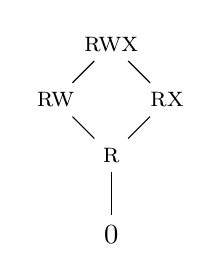
\begin{tikzpicture}[main node/.style={}]
    \node[main node] (rwx) {$\rwx$};
    \node[main node] (rx) [below right of=rwx] {$\rx$};

    \node[main node] (rw) [below left of=rwx,] {$\rw$};
    \node[main node] (r) [below right of=rw] {$\readonly$};
    \node[main node] (0) [below of=r] {$\noperm$};

    \path[every node/.style={font=\sffamily\small}]

    (rw) edge (r)
    (r) edge (0)

    (rwx) edge (rx)

    (rw) edge (rwx)
    (r) edge (rx);
  \end{tikzpicture}

  \caption{Permission hierarchy}
  \label{fig:perm-hier}
\end{wrapfigure}%
%
%%% Seals

Any reasonable capability machine needs a way to set up boundaries between security domains with different authorities.
It also must have a way to cross these boundaries such that (1) the security domain we move from can encapsulate itself and later regain its authority and (2) the security domain we move to regains all of its authority. 
%The M-Machine~\citep{Dally1997Memo59} inspired capability machine in \citet{skorstengaard_reasoning_2017} uses enter-capabilities to achieve this.
On \trgcm{} we have CHERI-like sealed capabilities to achieve this~\citep{watson_cheri_2015,watson_fast_2016}.
% seals
A sealed capability $\sealed{\sigma,\vsc}$ is a pair of a seal $\sigma$ (represented simply as a natural number) and a capability $\vsc$.
A sealed capability makes an underlying capability opaque which means that the underlying capability cannot be changed or used for the operations it normally gives permission to.
In other words, the authority the underlying capability represents is encapsulated under the seal.
In order to seal a capability with a seal $\sigma$, it is necessary to have the authority to do so.
The permission to make sealed capabilities is represented by a second form of capability in addition to the memory capabilities we saw above: a set-of-seals capability $\seal{\sigma_\var{base},\sigma_\var{end},\sigma_{\var{current}}}$.
Such a capability represents the authority to seal other capabilities with seals in the range $[\sigma_\var{base},\sigma_\var{end}]$.
In the spirit of memory capabilities, a set-of-seals capability has a current seal $\sigma_{\var{current}}$ that is selected for use in the next seal operation.
% On \trgcm{}, we represent seals in sets rather than single seals to have a more compact representation of multiple seals and make it possible to have seal allocation (not described here).
As we will see later, sealed capabilities get unsealed when they are invoked using an \texttt{xjmp}, an operation that operates on a pair of capabilities sealed with the same seal.
The instruction will be explained in more detail below, but essentially, it unseals the pair of capabilities, transfers control to one of them (the code part of the pair) and makes the other one (the data part) available to the invoked code.
The combination of sealed capabilities and \texttt{xjmp} gives us the properties (1) and (2) mentioned above: encapsulation of components' authority such that authority is restored upon invocation.
\begin{figure}[tb]
  \centering
  \[
  \arraycolsep=1.4pt
  \begin{array}{rrcl}
    \addrbnf,\basebnf \in & \Addr & \defeq & \nats \\
    \aendbnf & & \in & \Addr \cup \{\infty \}\\
    \permbnf \in& \Perm & \defbnf & \rwx \mid \rx \mid \rw \mid \ro \mid \noperm \\
    \linbnf && \defbnf & \linear \mid \normal\\
    \sealbasebnf, \sigma \in & \Seal & \defeq & \nats\\
    \sealendbnf & & \in & \Seal \cup \{\infty \}\\
    \vsc \in &\SealableCaps&\defbnf & ((\permbnf,\linbnf),\basebnf,\aendbnf,\addrbnf) \mid \seal{\sealbasebnf,\sealendbnf,\sigma}\\
    c \in&\Caps& \defbnf &  \SealableCaps \mid \sealed{\sigma,\scbnf}\\
    w \in &\Word & \defeq & \ints \uplus \Caps\\ 
    r \in& \RegName & \defbnf & \pcreg \mid \rretd \mid \rretc \mid \rstk \mid \rdata \mid \rtmp{1} \mid \rtmp{2} \mid \dots \\
    \reg \in &\Reg & \defeq & \RegName \fun \Word \\
    \mem \in&\Mem & \defeq & \Addr \fun \Word\\
    \ms \in  &\MemFrag & \defeq & \Addr \parfun \Word\\
    \Phi \in & \ExecConf & \defeq & \Mem \times \Reg\\
    &\Conf & \defeq & \ExecConf \cup \{\failed\} \cup \{\halted\} 
  \end{array}
\]
\[
  \arraycolsep=1.4pt
\begin{array}{rcl}
\multicolumn{3}{l}{    \arraycolsep=0pt
      \com{r} \in  \tRegName \hspace{2.5cm}   \com{\rn} \defbnf \com{r} \mid \nats
}\\
  \Instr &\defbnf & \tjmp{\com{r}} \mid \tjnz{\com{r}}{\com{\rn}} \mid \tmove{\com{r}}{\com{\rn}} \mid \tload{\com{r}}{\com{r}} \mid \tstore{\com{r}}{\com{r}} \mid \tplus{\com{r}}{\com{\rn}}{\com{\rn}} \mid \tminus{\com{r}}{\com{\rn}}{\com{\rn}} \mid\\
         & & \tlt{\com{r}}{\com{\rn}}{\com{\rn}} \mid \tisptr{\com{r}}{\com{r}} \mid\tgetp{\com{r}}{\com{r}} \mid \tgetlin{\com{r}}{\com{r}} \mid \tgetb{\com{r}}{\com{r}} \mid \tgete{\com{r}}{\com{r}} \mid \tgeta{\com{r}}{\com{r}}  \mid \\
  & & \tcca{\com{r}}{\com{n\rn}} \mid \tsetatob{\com{r}} \mid \trestrict{\com{r}}{\com{\rn}} \mid \tcseal{\com{r}}{\com{r}} \mid \txjmp{\com{r}}{\com{r}} \mid  \tsplit{\com{r}}{\com{r}}{\com{r}}{\com{\rn}} \mid\\ 
      & & \tsplice{\com{r}}{\com{r}}{\com{r}} \mid \tfail \mid \thalt 
\end{array}
\]
  \caption{The syntax of our capability machine with seals and linear capabilities.}
  \label{fig:target-syntax}
\end{figure}

%%% Domains
Words on \trgcm{} are either capabilities or data (represented by integers $\ints$).
% Instructions are stored in memory as integers and can be converted back and forth by unspecified $\encInstr{}$ and $\decInstr{}$ functions.
We assume a finite set of register names $\RegName$ containing at least the registers $\pcreg$, $\rretd$, $\rretc$, $\rstk$, $\rdata$, $\rtmp{1}$, and $\rtmp{2}$.
We define register files as functions from register names to words.
Complete memories map all addresses to words and memory fragments map some addresses to words (i.e.\ they are partial functions).
$\trgcm{}$ has two terminated configurations $\halted$ and $\failed$ that respectively signify a successful execution and an execution where something went wrong, e.g.,\ an out-of-bounds memory access.
An executable configuration is a register file and memory pair.

\begin{figure}
  \centering
  \begin{mathpar}
    \inference{\Phi(\pcreg) = ((\perm,\_),\baddr,\eaddr,\aaddr) \\
        \baddr \le \aaddr \le \eaddr \and \perm \in \{\rwx,\rx\}
 }{ \Phi \step \sem{\decInstr{\Phi.\mem(\aaddr)}}(\Phi) }
              \and
              \inference{ \forall \Phi' \neq \failed \ldotp \Phi \nrightarrow \Phi'}
                        {\Phi \step \failed }
  \end{mathpar}
  \[
    \begin{array}{l}
  %   \Phi \step
  % \begin{cases}
  %   \sem{\decInstr{\Phi.\mem(\aaddr)}}(\Phi) &
  %   \arraycolsep=0pt
  %     \begin{array}[t]{l}
  %       \text{if }\Phi(\pcreg) = ((\perm,\_),\baddr,\eaddr,\aaddr) \wedge
  %       \baddr \le \aaddr \le \eaddr \wedge \perm \in \{\rwx,\rx\}
  %     \end{array} \\
  %     \failed & \totherwise
  % \end{cases}\\
  \updPcAddr{\Phi} =
  \begin{cases}
    \Phi\updReg{\pcreg}{w} & \Phi(\pcreg) = ((\perm,\lin),\baddr,\eaddr,\aaddr) \wedge w = ((\perm,\lin),\baddr,\eaddr,\aaddr+1)\\
    \Phi  & \totherwise
  \end{cases}\\
  \linCons{w} =
  \begin{cases}
    0 & \isLinear{w} \\
    w & \totherwise
  \end{cases}\\
  \xjmpres{c_1,c_2,\Phi} =
  \begin{cases}
    \Phi\updReg{\pcreg}{c_1}\updReg{\rdata}{c_2} & \nonExec{c_2} \\
    \failed & \totherwise
  \end{cases}
  \end{array}
\]
\caption{An excerpt of the operational semantics of \trgcm{} (part 1/2).}
\label{fig:target-op-sem1}
\end{figure}

\begin{figure}
\begin{tabular}{|>{$}c<{$}|>{$}p{3cm}<{$}|>{\raggedright\arraybackslash}p{6cm}|}
    \hline
    i \in \Instr                                 & \sem{i}(\Phi) & Conditions\\
    \hline
    \halt                                        & \halted & \\
    \hline
    \fail                                        & \failed & \\
    % \hline
    % \move{r}{\rn}                                & \updPcAddr{\Phi\updReg{r}{\rn}} & $\rn \in \ints$\\
    \hline
  \move{r}{\rn}                                & \arraycolsep=0pt\array[t]{rl}\updPcAddr{}(&\\
  \Phi&\updReg{\rn}{w_2}\\ & \updReg{r}{w_1})\endarray & $\rn \in \RegName$ and $w_1 = \Phi(\rn)$ and $w_2 = \linCons{\Phi(\rn)}$ \\
    \hline
  \load{r_1}{r_2}                              & \arraycolsep=0pt\array[t]{rl}\updPcAddr{}(&\\
  \Phi&\updReg{r_1}{w_1}\\ &\update{\mem.\aaddr}{w_\aaddr})\endarray & $\Phi(r_2) = ((\perm,\_),\baddr,\eaddr,\aaddr)$ and $\baddr \le \aaddr \le \eaddr$ and $\perm \in \{\rwx,\rw,\rx,\ro\}$ and $w_1 = \Phi.\mem(\aaddr)$ and $\isLinear{w_1} \Rightarrow \perm \in \{\rwx,\rw\}$ and $w_a = \linCons{w_1}$\\
    \hline
  \store{r_1}{r_2}                             & \arraycolsep=0pt\array[t]{rl}&\updPcAddr{}(\\
  &\ \ \ \Phi\updReg{r_2}{w_2}\\ &\ \ \ \ \ \   \update{\mem.\aaddr}{\Phi(r_2)})\endarray & $\Phi(r_1) = ((\perm,\_),\baddr,\eaddr,\aaddr)$ and $\perm \in \{\rwx,\rw\}$ and $\baddr \le \aaddr \le \eaddr$ and $w_2 = \linCons{\Phi(r_2)}$\\
    \hline
  \geta{r_1}{r_2}                              & \arraycolsep=0pt\array[t]{rl}\updPcAddr{}&(\\
  &\Phi\updReg{r_1}{w})\endarray & If $\Phi(r_2) = ((\_,\_),\_,\_,\aaddr)$ or $\Phi(r_2) = \seal{\_,\_,\aaddr}$, then $w = \aaddr$ and otherwise $w = -1$\\
    \hline
  \cca{r}{\rn}                                 & \arraycolsep=0pt\array[t]{rl}\updPcAddr{}&(\\
  &\Phi\updReg{r}{w})\endarray & $\Phi(\rn) = n \in \ints$ and either $\Phi(r) = ((\perm,\lin),\baddr,\eaddr,\aaddr)$ or $\Phi(r) = \seal{\sigma_\baddr,\sigma_\eaddr,\sigma}$ and $w = ((\perm,\lin),\baddr,\eaddr,\aaddr + n)$ or $w = \seal{\sigma_\baddr,\sigma_\eaddr,\sigma+n}$, respectively \\
    \hline
    \jmp{r}    &\Phi\arraycolsep=0pt\array[t]{l}\updReg{r}{w}\\\updReg{\pcreg}{\Phi(r)}\endarray & $w = \linCons{\Phi(r)}$\\
    \hline
    \xjmp{r_1}{r_2}                              & \Phi' & $\Phi(r_1) = \sealed{\sigma,c_1}$ and $\Phi(r_2) = \sealed{\sigma,c_2}$ and $w_1 = \linCons{c_1}$ and $w_2 = \linCons{c_2}$ and $\Phi' = \xjmpres{c_1,c_2,\Phi\updReg{r_1,r_2}{w_1,w_2}}$  \\
    \hline
    \tsplit{r_1}{r_2}{r_3}{\rn}                  & \updPcAddr{}\arraycolsep=0pt\array[t]{rl}(\Phi&\updReg{r_3}{w}\\ &\updReg{r_1}{c_1}\\ &\updReg{r_2}{c_2})\endarray & $\Phi(r_3) = ((\perm,\lin),\baddr,\eaddr,\aaddr)$ and $\Phi(\rn) = n \in \nats$ and $\baddr \le n < \eaddr$ and $c_1 = ((\perm,\lin),\baddr,n,\aaddr)$ and $c_2 = ((\perm,\lin),n+1,\eaddr,\aaddr)$ and $w = \linCons{\Phi(r_3)}$\\
    \hline
    \splice{r_1}{r_2}{r_3}                       & \updPcAddr{}\arraycolsep=0pt\array[t]{rl}(\Phi&\updReg{r_2}{w_2}\\ &\updReg{r_3}{w_3}\\ &\updReg{r_1}{c})\endarray& $\Phi(r_2) = ((\perm,\lin),\baddr,n,\_)$ and $\Phi(r_3) = ((\perm,\lin),n+1,\eaddr,\aaddr)$ and $\baddr \le n < \eaddr$ and $c = ((\perm,\lin),\baddr,\eaddr,\aaddr)$ and $w_2,w_3 = \linCons{\Phi(r_2),\Phi(r_3)}$\\
    \hline
  \cseal{r_1}{r_2}                             & \arraycolsep=0pt\array[t]{rl}\updPcAddr{}&(\\
  &\Phi\updReg{r_1}{\vsc})\endarray & $\Phi(r_1) \in \SealableCaps$ and $\Phi(r_2) = \seal{\sigma_\baddr,\sigma_\eaddr,\sigma}$ and $\sigma_\baddr \le \sigma \le \sigma_\eaddr$ and $\vsc = \sealed{\sigma,\Phi(r_1)}$ \\
    \hline
    \multicolumn{3}{|c|}{\dots} \\
    \hline
    \_                                           & \failed & \totherwise \\
    \hline
  \end{tabular}
\caption{An excerpt of the operational semantics of \trgcm{} (part 2 of 2).}
  \label{fig:target-op-sem2}
\end{figure}
% syntax (instructions)
\trgcm{}'s instruction set is somewhat basic with the instructions one expects on most low-level machines as well as capability-related instructions.
The standard instructions are: unconditional and conditional jump (\texttt{jmp} and \texttt{jnz}), copy between registers (\texttt{move}), instructions that load from memory and store to memory (\texttt{load} and \texttt{store}), and arithmetic operations (\texttt{plus}, \texttt{minus}, and \texttt{lt}).
The simplest of the capability instructions inspect the properties of capabilities: type (\texttt{gettype}), linearity (\texttt{getl}), range (\texttt{getb} and \texttt{gete}), current address or seal (\texttt{geta}) or permission (\texttt{getp}).
The current address (or seal) of a capability (or set-of-seals) can be shifted by an offset (\texttt{cca}) or set to the base address (\texttt{seta2b}).
The \texttt{restrict} instruction reduces the permission of a capability according to the permission order $\le$.
Generally speaking, a capability machine needs an instruction for reducing the range of authority of a capability.
Because \trgcm{} has linear capabilities, the instruction for this splits the capability in two (\texttt{split}) rather than reducing the range of authority.
The reverse is possible using \texttt{splice}.
Sealables can be sealed using \texttt{cseal} and pairs of sealed capabilities can be unsealed by crossing security boundaries (\texttt{xjmp}, see below).
Finally, \trgcm{} has instructions to signal whether an execution was successful or not (\texttt{halt} and \texttt{fail}).

% opsem
The operational semantics of \trgcm{} is displayed in
Figures~\ref{fig:target-op-sem1} and~\ref{fig:target-op-sem2}.
The operational semantics is defined in terms of a step relation that executes the next instruction in an executable configuration $\Phi$ which results in a new executable configuration or one of the two terminated configurations.
The executed instruction is determined by the capability in the $\pcreg$ register, i.e.\ $\Phi(\pcreg)$ (we write $\Phi(r)$ to mean $\Phi.\reg(r)$).
In order for the machine to take a step, the capability in the $\pcreg$ must have a permission that allows execution, and the current address of the capability must be within the capability's range of authority.
If both conditions are satisfied, then the word pointed to by the capability is decoded to an instruction which is interpreted relative to $\Phi$.
The interpretations of some of the instructions are displayed in
Figure~\ref{fig:target-op-sem1} and~\ref{fig:target-op-sem2}.
In order to step through a program in memory, most of the interpretations use the function $\updPcAddr{}$ which simply updates the capability in the $\pcreg$ to point to the next memory address.
The instructions that stop execution or change the flow of execution do not use $\updPcAddr{}$.
For instance, the \texttt{halt} and \texttt{fail} instructions are simply interpreted as the $\halted$ and $\failed$ configurations, respectively, and they do not use $\updPcAddr{}$.

% move w/ lin
The \texttt{move} instruction simply moves a word from one register to another.
It is, however, complicated slightly by the presence of the non-duplicable linear capabilities.
When a linear capability is moved, the source register must be cleared to prevent duplication of the capability.
This is done uniformly in the semantics using the function $\linCons{}$ that returns $0$ for linear capabilities and is the identity for all other words.
When a word $w$ is transferred on the machine, then the source of $w$ is overwritten with $\linCons{w}$ which clears the source if $w$ was linear and leaves it unchanged otherwise.
In the case of \texttt{move}, the source register $\rn$ is overwritten with $\linCons{\Phi(\rn)}$.

% load w/ lin (and store)
The \texttt{store} and \texttt{load} instructions are fairly standard.
They require a capability with permission to either write or read depending on the operation, they check that the capability points within the range of authority.
Linear capabilities introduce one extra complication for \texttt{load} as it needs to clear the loaded memory address when it contains a linear capability in order to not duplicate the capability.
In this case, we require that the memory capability used for loading also has write-permission.

% geta, cca
The instruction \texttt{geta} projects the current address (or seal) from a capability (or set-of-seals), and returns $-1$ for data and sealed capabilities.
\texttt{cca} (change current address) changes the current address or seal of a capability or set-of-seals, respectively, by a given offset.
Note that this instruction does not need to use $\linCons{}$ like the previous ones, because it modifies the capability in-place, i.e.\ the source register is also the target register.
The \texttt{jmp} instruction is a simple jump that just sets register $\pcreg$.

%% Sealing
Two instructions manipulate seals in \trgcm{}: \texttt{cseal} for sealing a capability and \texttt{xjmp} for unsealing a pair of capabilities.
% cseal
Given a sealable $\vsc$ and a set-of-seals where the current seal $\sigma$ is within the range of available seals, the \texttt{cseal} instruction seals $\vsc$ with $\sigma$.
% xjmp
Apart from dealing with linearity, \texttt{xjmp} takes a pair of sealed capabilities, unseals them, and puts one in the $\pcreg$ register and the other in the $\rdata$ register, but only if they are sealed with the same seal and the data capability (the one placed in $\rdata$) is non-executable.
A pair of sealed capabilities can be seen as a closure where the code capability (the capability placed in $\pcreg$) is the program and the data capability is the local environment.
Because of the opacity of sealed capability, the creator of the closure can be sure that execution will start where the code capability points and only in an environment with the related data, i.e.\ sealed with the same seal.
This makes \texttt{xjmp} the mechanism on \trgcm{} that transfers control between security domains.
Opaque sealed capabilities encapsulate a security domain's local state and authority, and they only become accessible again when control is transferred to the security domain.
Some care should be taken for sealing because reusing the same seal for multiple closures makes it possible to jump to the code of one closure with the environment of another.
% xjmp to unseal
\trgcm{} does not have an instruction for unsealing capabilities directly, but we will explain below how it can be (partially) simulated using \texttt{xjmp}.

% split/splice
Instructions for reducing the authority of capabilities are commonplace on capability machines as they allow us to limit what a capability can do before it is passed away.
For normal capabilities, reduction of authority can be done without actually giving up any authority by duplicating the capability first.
With linear capabilities authority cannot be preserved in this fashion as they are non-duplicable.
In order to make a lossless reduction of the range of authority, \trgcm{} provides special hardware support in the form of \texttt{split} and \texttt{splice}.
The \texttt{split} instruction takes a capability with range of authority $[\var{base},\var{end}]$ and an address $n$ and creates two new capabilities, with $[\var{base},n]$ and $[n+1,\var{end}]$ as ranges of authority.
Everything else, i.e.\ permission, linearity and current address, is copied without change to the new capabilities.
With \texttt{split}, we can reduce the range of authority of a linear capability without losing any authority as we retain it in the second capability.
The \texttt{splice} instruction essentially does the inverse of \texttt{split}.
Given two capabilities with adjacent ranges of authority and the same permissions and linearity, \texttt{splice} splices them together into one capability.
The two instructions work in the same way for seal sets.
We do not provide special support for lossless reduction of capability permissions, but this could probably be achieved with more fine-grained permissions.
This would also allow linear capabilities to have aliases, but only by linear capabilities with disjoint permissions.

\begin{jversion}
% The remaining instructions
  The interpretation of the remainder of the instructions are displayed in Appendix~\ref{app:instr-interpretation}.
  The instructions $\tgetb{}{}$, $\tgete{}{}$, $\tgetlin{}{}$, and $\tgetp{}{}$ all project information about capabilities.
  The $\tgetb{}{}$ and $\tgete{}{}$ instructions, respectively, project the base and end address of the range of authority.
  The linearity of a permission is projected with $\tgetlin{}{}$, and finally the permission is projected with $\tgetp{}{}$.
  The instructions $\tgetb{}{}$ and $\tgete{}{}$ also work on sets of seals.
  The instruction $\tisptr{}{}$ returns an integer representation of the type of a word (capability or number).
  \trgcm{} also has arithmetic instructions $\tplus{}{}{}$, $\tminus{}{}{}$, and $\tlt{}{}{}$.
  The latter instruction compares two numbers and writes 1 or 0 to a target register depending on whether one number is less than the other.
  The instruction $\tsetatob{}$ sets the current address (or seal) of a capability (or set-of-seals) to the base address of the range of authority (or range of seals).
  This instruction makes it easy to work relatively to the base address of a capability.
  This instruction is not strictly necessary as it can be emulated with other instructions.
  Finally, we have the $\trestrict{}{}$ instruction which restricts the permission of a capability according to the $\le$ relation.
\end{jversion}

\begin{jversion}
  \subsection{The purpose of sealing}
  \label{sec:purpose-sealing}
  % Sealing example:
  To motivate the necessity of an encapsulation mechanism like sealing, consider the scenario where we are executing some trusted code and want to transfer control to untrusted code.
  We want to give the untrusted code the means to return to us.
  That is, we need to give them a return capability.
  For now, let us pretend that there does not exist a stack and only a single invocation of untrusted code happens in the entire execution.
  
  If we did not have an encapsulation mechanism, our only option would be to give the adversary an executable capability for the address we want them to return to.
  The untrusted code could use the return capability as intended, but it could also manipulate it to point elsewhere in our code.
  Jumping to such a capability could cause the trusted program to execute in an unintended and potentially insecure way.

  Additionally, when the untrusted code returns,  we need to regain access to the capabilities that represent our authority, which we had access to before passing control.
  To achieve this, we have to store them in a location that we can access after the return.
  However, without an encapsulation mechanism, the untrusted code would have access to all this through the return capability because it gives the same authority to the untrusted code as to us after the return.
  This is why any reasonable capability machine must have an encapsulation mechanism to allow programs to set up boundaries between security domains.
  
  In \trgcm{}, we can seal the return capability to establish such a boundary.
  Specifically, we can seal the return capability (which points to the instruction to be executed after the return) as a pair, together with a pointer to the stack frame where we have stashed away our capabilities (see further).
  By doing this, the untrusted code is prevented from changing the target of the return capability forcing them to return to the point we specified.
  Additionally, they do not get access to the capabilities we stashed away.
  Nevertheless, the automatic unsealing of sealed capability pairs upon invocation will ensure that the return code can still proceed as before.
  In other words, the sealing mechanism in \trgcm{} allows us to transfer control to untrusted code without giving up our capabilities or handing them over, and also control the locations in our code they can jump back to.

  It is worth pointing out that \trgcm{} does not have a direct unsealing instruction to extract a capability from its sealed version when the seal is available, but one can be emulated.
  Say you have a sealed non-executable word $\sealed{\sigma,w}$ as well as a set-of-seals capability $\seal{\sigma_\baddr,\sigma_\eaddr, \sigma}$ that contains $\sigma$, i.e.\ $\sigma \in [\sigma_\baddr,\sigma_\eaddr]$.
  It is possible to extract $w$ in $\rdata$ using $\txjmp{}{}$ in the following way.
  The idea is to use the seal to construct a sealed version of the pc capability incremented by one, and then perform an $\txjmp{}{}$ to it in combination with the sealed capability.
  This does not work for sealed executable capabilities because $\txjmp{}{}$ fails if the data capability is executable.
  However, even though we cannot extract the executable capability from $\sealed{\sigma,c}$, we can still invoke it with arbitrary arguments, since we can use the seal to construct an arbitrary data part and $\txjmp{}{}$ to the combination.\footnote{Alternatively, we could remove the current restriction in \texttt{xjmp} that requires the data capability to be non-executable but then teh invoked code would often have to manually perform this check instead.}

  Sealing is meant for encapsulation, but it relies on seals being kept private as should be clear from the explanations so far.
  For this reason, it is important that trusted code does not leak its seals to adversaries and that the system is initialised so that each component has access to unique seals.
  We return to this in \sectionname~\ref{sec:well-form-reas}.
\end{jversion}

\begin{jversion}
\subsection{Decoding and encoding functions}
The operational semantics of the capability machine uses the function $\decInstr{}$ to decode instructions.
We also assume a function $\encInstr{}$ to make it easy to specify programs in terms of instructions.
Rather than defining such a decode function and an encode function, we assume that they are given with certain properties.
The $\decInstr{} : \Word \fun \Instr$ should decode all capabilities to the $\fail$ instruction, i.e.\ only numbers are decoded to non-fail instructions:
\[
\forall c \in \Caps \ldotp \decInstr{c} = \fail
\]
The $\decInstr{}$ should have a right inverse $\encInstr{} : \Instr \fun \ints$, i.e.
\[
\forall i \in \Instr \ldotp \decInstr{}(\encInstr{i}) = i
\]
These assumptions are sufficient to construct program examples in terms of instructions rather than machine words (using $\encInstr{}$), and run them on the machine (using the fact that $\decInstr{}$ is the left inverse of $\encInstr{}$).
% The $\encInstr{}$ function allows us to specify the program ``abstractly''.
% As the $\decInstr{}$ function is the left inverse of $\encInstr{}$, we can even execute the program in the operational semantics without ever worrying about what the actual encoding is.
%This is not to say that encoding is an easy problem. There are many things to get.

The full machine semantics in Appendix~\ref{app:instr-interpretation} also assumes decode and encode functions for permissions $\encPerm{} : \Perm \fun \ints$ and $\decPerm{} : \ints \fun \Perm$.
We assume the $\decPerm{}$ function to be the left inverse of $\encPerm{}$.
For $\encPerm{}$, we assume that it does not encode anything to the $\tgetp{}{}$ error value -1, i.e.
\[
  \forall \perm \in \Perm \ldotp \encPerm{\perm} \neq -1
\]
For linearity we assume similar functions.
Finally in the interpretation of $\tisptr{}{}$, the machine uses an encode function for word types $\encType{}$.
This function encodes each kind of word as an integer.
This is very much like the previous functions.
It encodes each kind of word differently and all words of the same kind to the same integer.
\end{jversion}

\subsection{Components, linking, programs, and contexts}
\label{subsec:components-linking}
The executable configuration describes the machine state, but it does not make it clear what components run on the machine and how they interact with each other.
To clarify this, we introduce notions of components and programs from which we construct executable configurations.
A component (defined in Figure~\ref{fig:target-component-and-linking}) is basically a program with entry points in the form of imports that need to be linked.
It has exports that can satisfy the imports of other components.
% Structure
A base component $\comp_0$ consists of a code memory fragment, a data memory fragment, a list of imported symbols, a list of exported symbols, two lists specifying the available seals (see Section~\ref{sec:form-secur-with}), and a set of all the linear addresses (addresses governed by a linear capability).
The import list specifies where in memory imports should be placed, and imports are matched to exports via their symbols.
An export associates a word with a symbol.
%base = library
A component is either a library component (without a main entry point) or an incomplete program with a main in the form of a pair of sealed capabilities.
The latter can be seen as a program that still needs to be linked with libraries.
% Linking .
Components are combined into new components by linking them together, as long as only one has a main function.
Two components can be linked when their memories, seals, and linear addresses are disjoint.
They are combined by taking the union of each of their constituents.
For every import that is satisfied by an export of the other component, the data memory is updated to have the exported word on the imported address.
The satisfied imports are removed from the import list in the resulting linked component and the exports are obtained by combining the components' exports.

% Programs
We can now define the notion of a program as well as a context.
\begin{definition}[Programs and Contexts]
  \label{def:program-and-context}
  A \emph{program} is a component $(\comp_0,c_{\mathrm{main},c}, c_{\mathrm{main},d})$ with an empty import list.
  A \emph{context} for a component $\comp$ is a component $\comp'$ such that $\comp \bowtie \comp'$ is a program.
\end{definition}
% Getting an executable from a component - postpone this to later, but mention:
% write xor exec
How a program is initialised to create an executable configuration is discussed in Section~\ref{sec:form-secur-with}.
% We will, however, at this point mention that all programs will be instrumented as Write-XOR-Execute,{Do we have a reference for this?} i.e.\ there will only be read-execute capabilities for the code and read-write capabilities for the data.
%Further, we will only consider a specific class of well-formed components, but we will get back to this.
Some simplifications have been made in this presentation of \trgcm{}. See \citet{technical_report_popl} for details.
\begin{figure}[tb]
  \centering
  \[
    \begin{array}{rl c rl c rl}
    s &\in \Symbol & \phantom{make} &
    \mathrm{import} &\mathrel{::=} a \mapsfrom s & \phantom{make} &
    \mathrm{export} &\mathrel{::=} s \mapsto w\\
    \comp_0 & \multicolumn{7}{l}{\mathrel{::=} (\mscode,\msdata,\overline{\mathrm{import}},\overline{\mathrm{export}},\sigrets,\sigcloss,A_\linear)}\\
    \comp & \multicolumn{7}{l}{\mathrel{::=} \comp_0 \mid  (\comp_0,c_{\mathrm{main},c}, c_{\mathrm{main},d})}
  \end{array}
\]
\vspace{0.5cm}
\begin{mathpar}
  \inference{
    \comp_0 = (\mscode[1], \msdata[1], \overline{\var{import}_1}, \overline{\var{export}_1}, \sigrets[1], \sigcloss[1],A_{\linear,1})\\
    \comp_0' = (\mscode[2], \msdata[2], \overline{\var{import}_2}, \overline{\var{export}_2}, \sigrets[2], \sigcloss[2],A_{\linear,2})\\
    \comp_0'' = (\mscode[3], \msdata[3], \overline{\var{import}_3}, \overline{\var{export}_3}, \sigrets[3], \sigcloss[3],A_{\linear,3})\\
    \mscode[3] = \mscode[1] \uplus \mscode[2] \\
    \msdata[3] = (\msdata[1] \uplus \msdata[2])[a \mapsto w \mid (a \mapsfrom s) \in (\overline{\var{import}_1} \cup \overline{\var{import}_2}), (s \mapsto w) \in \overline{\var{export}}_3] \\
    \overline{\var{export}_3} = \overline{\var{export}_1} \cup \overline{\var{export}_2}&
    \overline{\var{import}_3} = \{ a \mapsfrom s \in (\overline{\var{import}_1} \cup \overline{\var{import}_2}) \mid s \mapsto \_ \not\in \overline{\var{export}_3} \}\\
    \sigrets[3] = \sigrets[1] \uplus \sigrets[2] &
    \sigcloss[3] = \sigcloss[1] \uplus \sigcloss[2] &
    A_{\linear,3} = A_{\linear,1} \uplus A_{\linear,2}\\
    \dom(\mscode[3]) \mathrel{\#} \dom(\msdata[3]) & \sigrets[3] \mathrel{\#} \sigcloss[3]
  } {
    \comp_0'' = \comp_0 \bowtie \comp_0'
  }
  \and
  \inference{
    \comp_0'' = \comp_0 \bowtie \comp_0'
  }{
    \begin{aligned}
      (\comp_0'',c_{\mathrm{main},c}, c_{\mathrm{main},d}) &= \comp_0 \bowtie
      (\comp_0',c_{\mathrm{main},c}, c_{\mathrm{main},d})\\
      &=
      (\comp_0,c_{\mathrm{main},c}, c_{\mathrm{main},d}) \bowtie \comp_0'
    \end{aligned}
  }
  \end{mathpar}
% \begin{definition}[Plugging a program into a context]
%   When $\var{comp'}$ is a context for component $\comp$ and $\comp' \bowtie \comp \rightsquigarrow \Phi$, 
%   then we write $\plug{\comp'}{\comp}$ for the execution configuration $\Phi$.
% \end{definition}
  \caption{Components and linking of components.}
  \label{fig:target-component-and-linking}
\end{figure}

%\FloatBarrier
% \begin{itemize}
% \item present our \emph{target language} and its operational semantics (excerpts)
% \item mention roughly what components look like
% \end{itemize}
\section{Linear Stack and Return Capabilities}
\label{sec:stktokens-explained}
In this section, we introduce our calling convention \stktokens{} that ensures LSE and WBCF.
We will gradually explain each of the security measures \stktokens{} takes and motivate them with the attacks they prevent.

\begin{figure}
  \centering
  \begin{subfigure}{0.45\linewidth}
    \centering
    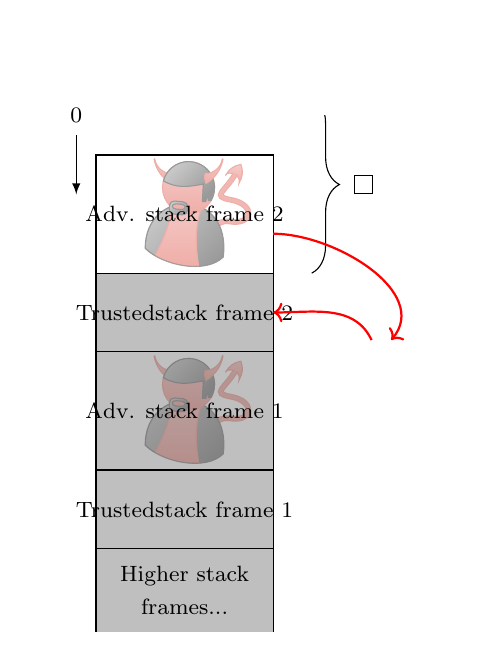
\begin{tikzpicture}[scale=.5, every node={scale=.5}]
      % recurrent parts
      \draw (-0.5,13) node {\footnotesize 0};
      \draw (-0.5,12.5) edge[thin,-latex] (-0.5,11);
      \stdstackstart[13]
      \inactsf{(0,2)}{(4.5,4)} {\footnotesize Trusted\\ \footnotesize stack frame 1}
      \inactadv{(0,4)}{(4.5,7)} {\footnotesize Adv. stack frame 1}
      \inactsf{(0,7)}{(4.5,9)} {\footnotesize Trusted \\ \footnotesize stack frame 2}
      \actadv{(0,9)}{(4.5,12)} {\footnotesize Adv. stack frame 2}

      % Stack pointer 1
      \begin{scope}
        \clip (4.6,4) rectangle (9,13);
        \capbracebot{(4.6,4)}{(4.6,13.5)}{adv. stack\\\footnotesize cap. 1}
      \end{scope}
      Stack pointer 2
      \begin{scope}
        \clip (4.8,4) rectangle (9,13);
        \capbrace{(5.2,9)}{(5.2,13.5)}{adv. stack\\\footnotesize cap. 2}
      \end{scope}

      \draw[red,thick,->] (4.5,10) to[out=0,in=50] node[midway,right] {} (7.5,7.3);
      \draw[red,thick,->] (7,7.3) to[out=115,in=0] node[midway,right] {} (4.5,8);
    \end{tikzpicture}
    \caption{An adversary uses a previous stack frame's stack pointer.}
    \label{fig:stack-ptr-abuse}
  \end{subfigure}
  \begin{subfigure}{0.08\linewidth}
    \phantom{testtestes}
  \end{subfigure}
  \begin{subfigure}{0.45\linewidth}
    \centering
    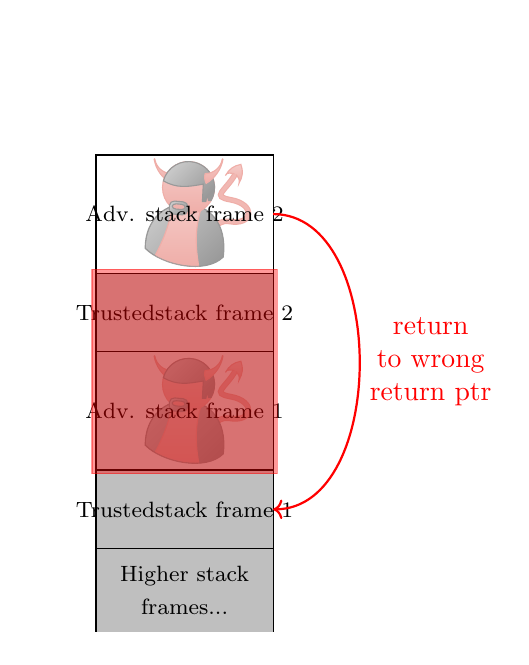
\begin{tikzpicture}[scale=.5, every node={scale=.5}]
      % recurrent parts
      \stdstackstart[13]
      \inactsf{(0,2)}{(4.5,4)} {\footnotesize Trusted\\ \footnotesize stack frame 1}
      \inactadv{(0,4)}{(4.5,7)} {\footnotesize Adv. stack frame 1}
      \inactsf{(0,7)}{(4.5,9)} {\footnotesize Trusted \\ \footnotesize stack frame 2}
      \actadv{(0,9)}{(4.5,12)} {\footnotesize Adv. stack frame 2}
      \fill[red,draw=red,opacity=.4] (-.1,3.9) rectangle (4.6,9.1);
      \draw[red,thick,->] (4.5,10.5) to[out=0,in=0] node[midway,right,align=center] {return\\ to wrong\\ return ptr} (4.5,3);
    \end{tikzpicture}
    \caption{An adversary jumps to a previous stack frame's stack pointer.}
    \label{fig:ret-ptr-abuse}
  \end{subfigure}
  
  \caption{Possible ways to abuse stack and return capabilities.
    Grey and white frames indicate inactive and active stack frames respectively.
    The red frame emphasizes stack frames being skipped by an adversarial return.}
  \label{fig:stack-ret-ptr-abuse}
\end{figure}

\stktokens{} is based on a traditional single stack, shared between all components.
To explain the technique, let us first consider how we might already add extra protection to stack and return pointers on a capability machine.
First, we replace stack pointers with stack capabilities.
When a new stack frame is created, the caller provisions it with a stack capability, restricted to the appropriate range, i.e.\ not covering the caller's stack frame.
Return pointers, on the other hand, are replaced by a pair of sealed return capabilities, as explained in Section~\ref{sec:purpose-sealing}.
% KJAA: Again with the sealed pair. Again, this idea is unclear.
They form an opaque closure that the callee can only jump to, and when that happens, the caller's data becomes available to the caller's return code. 

%informally explain how an adversary may try to abuse stack and return caps
While the above adds extra protection, it is not sufficient to enforce WBCF and LSE.
Untrusted callees receive a stack capability and a return pair that they are supposed to use for the call.
However, a malicious callee (which we will refer to as an adversary\footnote{See Section~\ref{sec:well-form-reas} for more details on our attacker model.}) can store the provided capabilities away on the heap in order to use them later.
Figure~\ref{fig:stack-ret-ptr-abuse} illustrates two examples of this.
In both examples our component and an adversarial component have been taking turns calling each other, so the stack now contains four stack frames alternating between ours and theirs.
The figure on the left (Figure~\ref{fig:stack-ptr-abuse}) illustrates how we try to ensure LSE by restricting the stack capability to the unused part before every call to the adversary.
However, restricting the stack capability does not help when we, in the first call, give access to the part of the stack where our second stack frame will reside as nothing prevents the adversary from duplicating and storing the stack pointer.
Generally speaking, we have no reason to ever trust a stack capability received from an untrusted component as that stack capability may have been duplicated and stored for later use.
In the figure on the right (Figure~\ref{fig:ret-ptr-abuse}), we have given the adversary two pairs of sealed return capabilities, one in each of the two calls to the adversarial component.
The adversary stores the pair of sealed return capabilities from the first call in order to use it in the second call where they are not allowed.
The figure illustrates how the adversarial code uses the return pair from the first call to return from the second call and thus break WBCF.

% Informally explain how we prevent this using linear capabilities
As the examples illustrate, this naive use of memory and object capabilities does not suffice to enforce LSE and WBCF.
The problem is essentially that the stack and return pointers that a callee receives from a caller remain in effect outside their intended lifetime: either when the callee has already returned or when they have themselves invoked other code. 
Linear capabilities offer a form of revocation\footnote{Revocation in the sense that if we hand out a linear capability and later get it back, then the receiver cannot have kept a copy of it as it is non-duplicable.} that can be used to prevent this from happening.

% Stack capability linear
The linear capabilities are put to use by requiring the stack capability to be linear.
On call, the caller splits the stack capability in two: one capability for their local stack frame and another one for the unused part of the stack.
The local stack frame capability is sealed and used as the data part of the sealed return pair.
The capability for the remainder of the stack is given to the callee.
% Prevention of left attack non-aliasing of linear capabilities - token like (ensuring LSE)
Because the stack capability is linear, the caller knows that the capability for their local stack frame cannot have an alias.
This means that an adversary would need the stack capability produced by the caller in order to access their local data.
The caller gives this capability to the adversary only in a sealed form, rendering it opaque and unusable.
This is illustrated in Figure~\ref{fig:stack-ptr-abuse-prev} and prevents the issue illustrated in Figure~\ref{fig:stack-ptr-abuse}.

% Prevention of attack 2
In a traditional calling convention with a single stack, the stack serves as a call stack keeping track of the order calls were made in and thus in which order they should be returned to.
A caller pushes a stack frame to the stack on call and a callee pops a stack frame from the stack upon return.
However without any enforcement, there is nothing to prevent a callee from returning from an arbitrary call on the call stack.
This is exactly what the adversary does in Figure~\ref{fig:ret-ptr-abuse} when they skip two stack frames.
In the presence of adversarial code, we need some mechanism to enforce that the order of the call stack is kept.
One way to enforce this would be to hand out a token on call that can only be used when the caller's stack frame is on top of the call stack.
The callee would have to present this token on return to prove that it is allowed to return to the caller, and on return the token would be taken back by the caller to prevent it from being spent multiple times.
As it turns out, the stack capability for the unused part of the stack can be used as such a token in the following way:
On return the callee has to give back the stack capability they were given on invocation.
When the caller receives a stack capability back on return, it checks that this token is actually spendable, i.e.\ whether its stack frame is on top of the logical call stack or not.
This check can be done by attempting to recombine (splice) the return token with the stack capability for the local stack frame (which at this point has been unsealed again) in order to reconstruct the original stack capability.
If the splice is successful, then the caller knows that the two capabilities are adjacent. On the other hand, if the splice fails, then they are alerted to the fact that their stack frame may not be the topmost.
\stktokens{} uses this approach; and as illustrated in Figure~\ref{fig:ret-ptr-abuse-prev}, it prevents the issue in Figure~\ref{fig:ret-ptr-abuse} as the adversary does not return a spendable token when they return.
\begin{figure}
  \centering
  \begin{subfigure}{0.45\linewidth}
    \centering
    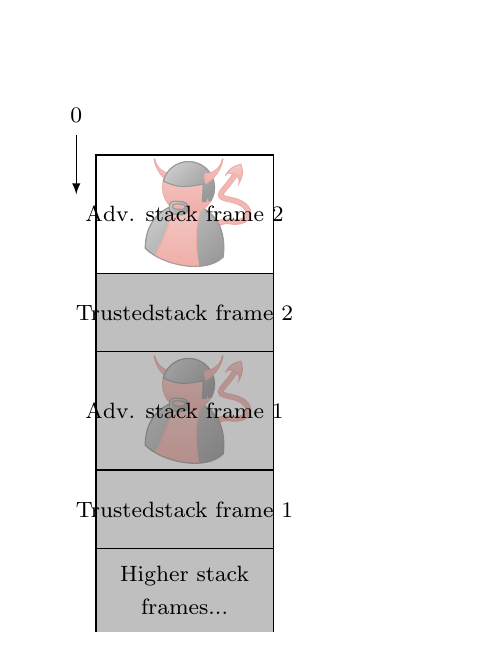
\begin{tikzpicture}[scale=.5, every node={scale=.5}]
      % recurrent parts
      \draw (-0.5,13) node {\footnotesize 0};
      \draw (-0.5,12.5) edge[thin,-latex] (-0.5,11);
      \stdstackstart[13]
      \inactsf{(0,2)}{(4.5,4)} {\footnotesize Trusted\\ \footnotesize stack frame 1}
      \inactadv{(0,4)}{(4.5,7)} {\footnotesize Adv. stack frame 1}
      \inactsf{(0,7)}{(4.5,9)} {\footnotesize Trusted \\ \footnotesize stack frame 2}
      \actadv{(0,9)}{(4.5,12)} {\footnotesize Adv. stack frame 2}

      \sealsymb{(4.9,3)}
      \lincapbrace{(4.6,2)}{(4.6,4)}{data return\\\footnotesize cap. 1}

      % Stack pointer 1
      \sealsymb{(4.9,5.5)}
      \lincapbrace{(4.6,4)}{(4.6,7)}{adv. stack\\\footnotesize cap. 1}
      % return cap
      \sealsymb{(4.9,8)}
      \lincapbrace{(4.6,7)}{(4.6,9)}{data return\\\footnotesize cap. 2}
     %  Stack pointer 2
      \begin{scope}
        \clip (4.8,4) rectangle (9,13);
        \lincapbrace{(4.6,9)}{(4.6,13.5)}{adv. stack\\\footnotesize cap. 2}
      \end{scope}

    \end{tikzpicture}
    \caption{The non-duplicable linear stack capability for the trusted code's
      stack frame and the opacity of sealed capabilities ensures LSE.}
    \label{fig:stack-ptr-abuse-prev}
  \end{subfigure}
  \begin{subfigure}{0.08\linewidth}
    \phantom{testtestes}
  \end{subfigure}
  \begin{subfigure}{0.45\linewidth}
    \centering
    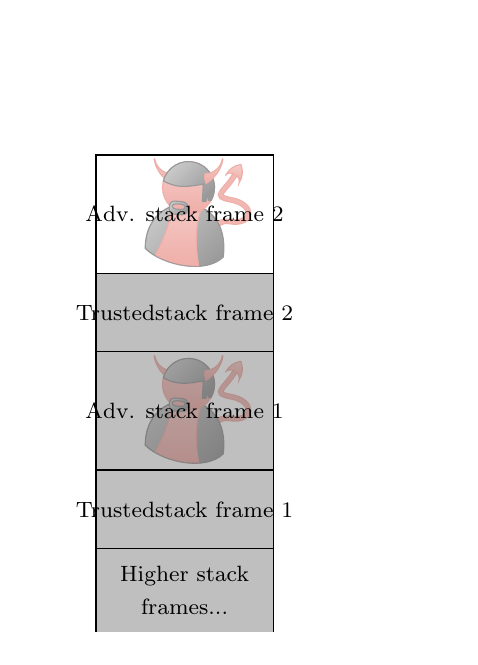
\begin{tikzpicture}[scale=.5, every node={scale=.5}]
      % recurrent parts
      \stdstackstart[13]
      \inactsf{(0,2)}{(4.5,4)} {\footnotesize Trusted\\ \footnotesize stack frame 1}
      \inactadv{(0,4)}{(4.5,7)} {\footnotesize Adv. stack frame 1}
      \inactsf{(0,7)}{(4.5,9)} {\footnotesize Trusted \\ \footnotesize stack frame 2}
      \actadv{(0,9)}{(4.5,12)} {\footnotesize Adv. stack frame 2}

      \lincapbrace{(4.6,2)}{(4.6,4)}{data return\\\footnotesize cap. 1}

     %  Stack pointer 2
      \begin{scope}
        \clip (4.8,4) rectangle (9,13);
        \lincapbrace{(4.6,9)}{(4.6,13.5)}{adv. stack\\\footnotesize cap. 2}
      \end{scope}

      \redcross{(5,4)}
    \end{tikzpicture}
    \caption{The trusted caller fails to splice the stack capability returned by
    the adversary with the capability for the trusted caller's local stack frame.}
    \label{fig:ret-ptr-abuse-prev}
  \end{subfigure}
  \caption{Abuse of stack and return capabilities prevention.
    Grey and white frames indicate inactive and active stack frames respectively.
    Linear braces indicate memory owned by linear capabilities.  
  }
\end{figure}

% Non-empty trusted stack frames.
In order for a call to have a presence on the call stack, its stack frame must be non-empty.
We cannot allow empty stack frames on the call stack, because then it would be impossible to tell whether the topmost non-empty stack frame has an empty stack frame on top of it.
Non-empty stack frames come naturally in traditional C-like calling convention as they keep track of old stack pointers and old program counters on the stack, but in \stktokens{} these things are part of the return pair which means that a caller with no local data may only need an empty stack frame.
In other words, a caller using \stktokens{} needs to take care that their stack frame is non-empty in order to reserve their spot in the return order.
There is also a more practical reason for a \stktokens{} caller to make sure their stack frame is non-empty: They need a fragment of the stack capability in order to perform the splice that verifies the validity of the return token.

\begin{figure}
  \centering
  \begin{subfigure}{0.23\linewidth}
    \centering
    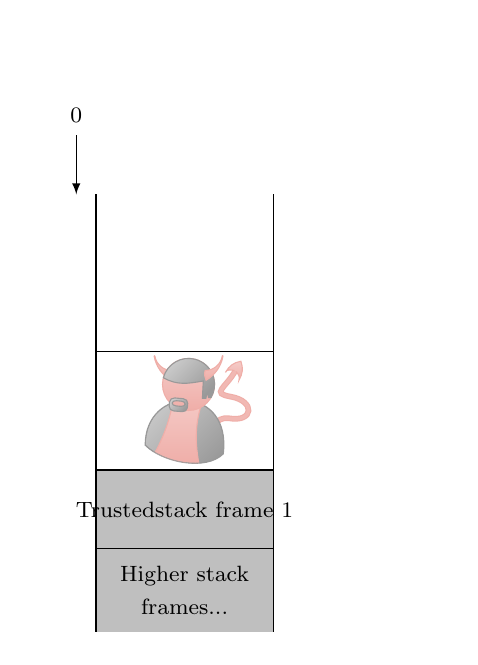
\begin{tikzpicture}[scale=.5, every node={scale=.5}]
      % recurrent parts
      \draw (-0.5,13) node {\footnotesize 0};
      \draw (-0.5,12.5) edge[thin,-latex] (-0.5,11);
      \stdstackstart[13]
      \inactsf{(0,2)}{(4.5,4)} {\footnotesize Trusted\\ \footnotesize stack frame 1}
      \actadv{(0,4)}{(4.5,7)}{}

      \sealsymb{(4.9,3)}
      \lincapbrace{(4.6,2)}{(4.6,4)}{}
      \begin{scope}
        \clip (4.8,1) rectangle (9,13);
      \lincapbracebot{(4.6,4)}{(4.6,13.5)}{}
      \end{scope}

    \end{tikzpicture}
    \caption{}
    \label{fig:stack-base-abuse-a}
  \end{subfigure}
  \begin{subfigure}{0.24\linewidth}
    \centering
    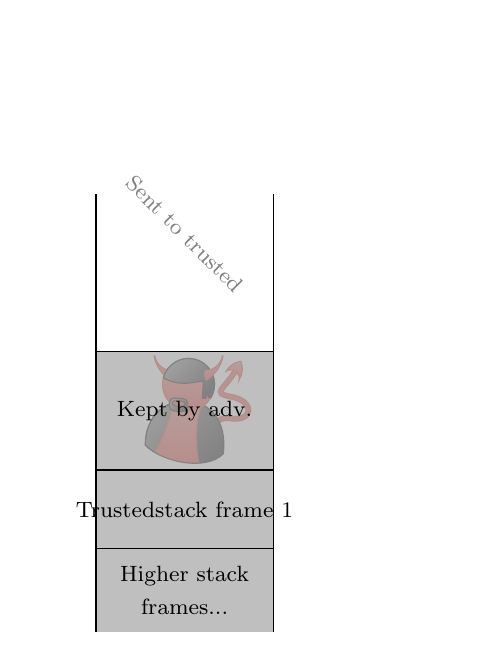
\begin{tikzpicture}[scale=.5, every node={scale=.5}]
      % recurrent parts
      \stdstackstart[13]
      \inactsf{(0,2)}{(4.5,4)} {\footnotesize Trusted\\ \footnotesize stack frame 1}
      \inactadv{(0,4)}{(4.5,7)}{\footnotesize Kept by adv.}
      \node[opacity=0.5,rotate=-45] at (2.25,10) {\footnotesize Sent to trusted};

      \sealsymb{(4.9,3)}
      \lincapbrace{(4.6,2)}{(4.6,4)}{}
      \lincapbrace{(4.6,4)}{(4.6,7)}{}
      
      \begin{scope}
        \clip (4.8,1) rectangle (9,13);
      \lincapbracebot{(4.6,7)}{(4.6,13.5)}{}
      \end{scope}

    \end{tikzpicture}
    \caption{}
    \label{fig:stack-base-abuse-b}
  \end{subfigure}
  \begin{subfigure}{0.24\linewidth}
    \centering
    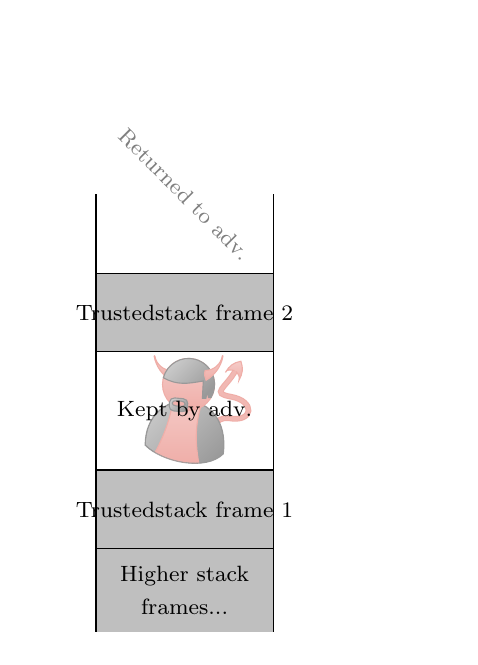
\begin{tikzpicture}[scale=.5, every node={scale=.5}]
      % recurrent parts
      \stdstackstart[13]
      \inactsf{(0,2)}{(4.5,4)} {\footnotesize Trusted\\ \footnotesize stack frame 1}
      \actadv{(0,4)}{(4.5,7)}{\footnotesize Kept by adv.}
      \inactsf{(0,7)}{(4.5,9)} {\footnotesize Trusted\\ \footnotesize stack frame 2}
      \node[opacity=0.5,rotate=-45] at (2.25,11) {\footnotesize Returned to adv.};
      \sealsymb{(4.9,3)}
      \lincapbrace{(4.6,2)}{(4.6,4)}{}
      \lincapbrace{(4.6,4)}{(4.6,7)}{}

      \sealsymb{(4.9,8)}
      \lincapbrace{(4.6,7)}{(4.6,9)}{}
      \begin{scope}
        \clip (4.8,1) rectangle (9,13);
        \lincapbracebot{(4.6,9)}{(4.6,13.5)}{}
      \end{scope}

    \end{tikzpicture}
    \caption{}
    \label{fig:stack-base-abuse-c}
  \end{subfigure}
  \begin{subfigure}{0.24\linewidth}
    \centering
    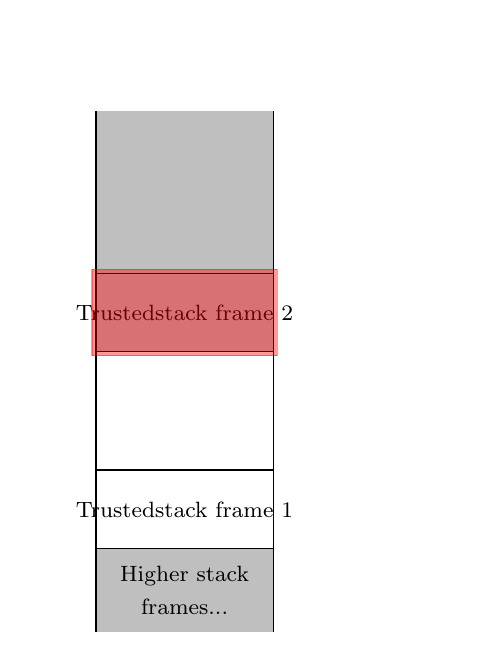
\begin{tikzpicture}[scale=.5, every node={scale=.5}]
      % recurrent parts
      \stdstackstart[13]
      \actsf{(0,2)}{(4.5,4)} {\footnotesize Trusted\\ \footnotesize stack frame 1}

      \inactsf{(0,7)}{(4.5,9)} {\footnotesize Trusted\\ \footnotesize stack frame 2}
      \begin{scope}
        \clip (-.1,-.1) rectangle (4.6,13.1);
        \draw[fill=gray!50] (0,9) rectangle (4.5,13.5);
      \end{scope}

      \lincapbrace{(4.6,2)}{(4.6,7)}{}

      \sealsymb{(4.9,8)}
      \lincapbrace{(4.6,7)}{(4.6,9)}{}

      \fill[red,draw=red,opacity=.4] (-.1,6.9) rectangle (4.6,9.1);
      \begin{scope}
        \clip (4.8,1) rectangle (9,13);
        \lincapbracebot{(4.6,9)}{(4.6,13.5)}{}
      \end{scope}

    \end{tikzpicture}
    \caption{}
    \label{fig:stack-base-abuse-d}
  \end{subfigure}
  \caption{Partial return token used to return out of order.
    Grey and white frames indicate inactive and active stack frames respectively.
    Linear braces indicate memory owned by linear capabilities.
    The red frame emphasizes a stack frame that is being skipped by an adversarial return.
  }
  \label{fig:stk-base-abuse}
\end{figure}

% known stack base
% + more
At this point, the caller checks that the return token is adjacent to the stack capability for the caller's local stack frame and they have the means to do so.
However, this still does not ensure that the caller's stack frame is on top of the call stack.
The issue is that stack frames may not be tightly packed leaving space between stack frames in memory.
An adversarial callee may intentionally leave a bit of space in memory above the caller's stack frame, so that they can later return out of order by returning the bit of the return token for the bit of memory left above the caller's stack frame.
This is illustrated in Figure~\ref{fig:stk-base-abuse}: In Figure~\ref{fig:stack-base-abuse-a}, a trusted caller has called an adversarial callee.
The adversary calls the trusted code back, but first they split the return token in two and store on the heap the part for the memory adjacent to the trusted caller's call frame (Figure~\ref{fig:stack-base-abuse-b}).
The trusted caller calls the adversary back using the precautions we have described so far (Figure~\ref{fig:stack-base-abuse-c}).
At this point (Figure~\ref{fig:stack-base-abuse-d}), the adversary has access to a partial return token adjacent to the trusted caller's first stack frame which allows the adversary to return from this call breaking WBCF.

For the caller to be sure that there are no hidden stack frames above its own, they need to make sure that the return token is exactly the same as the one they passed to the callee.
In \stktokens{}, the base address of the stack capability is fixed as a compile-time constant (Note: the stack grows downwards, so the base address of the stack capability is the top-most address of the stack). 
The caller verifies the validity of the return token by checking whether the base address of a returned token corresponds to this fixed base address, which was the base address for the return token they gave to the callee.
In the scenario we just sketched, the caller would be alerted to the attempt to break WBCF when the base address check of the return token fails in Figure~\ref{fig:stack-base-abuse-d}.

% Where do we get the stack pointer from, how can we know it is linear
% The other attack.
% At this point, the caller is able to verify whether a return token is spendable which allows them to decide whether they have the topmost stack frame on a call stack.
% However, in order to have WBCF there should only be one call stack, so the caller should also be able to verify that they have the top stack frame on the call stack used by all well-behaved components.
% In case a trusted component did not start the execution on the machine, i.e.\ they were called by another component, then the trusted component has no way to be sure whether the stack capability passed to them corresponds to the one and only call stack.
% To illustrate how an adversarial component can break WBCF by using multiple different stack capabilities consider this example: An adversary calls a trusted component with a callback and some linear capability that they claim is the stack capability.
% The trusted component executes using the stack capability given to them and at some point they invoke the callback, creating return tokens and so on.
% The adversary stores the return pair and return token and calls another trusted component but with a new callback and a new linear capability that they claim is the stack capability.
% Again, this trusted component also executes using the stack capability given to them and at some point they too invoke the callback, taking all the precautions we have described so far.
% At this point, the adversary has everything they need to return from either of the two callbacks.
% Specifically, they could return from the first callback invocation before they have returned from the second, breaking WBCF.
% From a high-level perspective, the problem is that both trusted components will be able to verify that they have the top stack frame on the call stack.
% They are both correct as the adversarial component has created two call stacks, one for each of the components.
% In order to solve this problem, the well-behaved code needs to somehow agree on the call stack.
% We do this by statically deciding on a global base address for the stack which is used for the entirety of the execution.
% A caller makes sure that they are using the correct stack by checking that the base address of the stack capability they receive corresponds to the global stack base address.
% This also means that on every return, the caller will check whether the return token's base address is equal to the global stack address.

In \stktokens{}, the stack memory is only referenced by a single linear stack capability at the start of execution.
Because of this, the return token can be verified simply by checking its base address and splicing it with the caller's stack frame.
There is no need to check linearity because only linear capabilities to this memory exist.

% Return pointers/return seals
The return pointer in the \stktokens{} scheme is a pair of sealed capabilities where the code part of the pair is the old program counter, and the data part is the stack capability for the local stack frame of the caller.
Both of the capabilities in the pair are sealed with the same seal.
% One seal per return point
All call points need to be associated with a unique seal (a return seal) that is only used for the return capabilities for that particular call point.
The return seal is what associates the stack frame on the call stack with a specific call point in a program, so if we allowed return seals to be reused, it would be possible to return to a different call point than the one that gave rise to the stack frame, breaking WBCF.
For similar reasons, we cannot allow return seals to be used to seal closures.
% Don't be stupid
Return seals should never be leaked to adversarial code as this would allow them to unseal the local stack frame of a caller breaking LSE.
This goes for direct leaks (leaving a seal in a register or writing it to adversarial memory), as well as indirect leaks (leaking a different capability that can be used for reading, either directly or indirectly, a return seal from memory).

% Note about them vs us, we do nothing that they couldn't do
We have sometimes phrased the description of the \stktokens{} calling scheme in terms of ``them vs us''.
This may have created the impression of an asymmetric calling convention that places a special status on trusted components allowing them to protect themselves against adversaries.
However, \stktokens{} is a modular calling scheme: no restriction is put on adversarial components that we do not expect trusted components to meet.
Specifically, we will only assume that both trusted and adversarial components are initially syntactically well-formed (described in more detail in Section~\ref{sec:well-form-reas}) which basically just ensures that their initial state does not break machine guarantees (e.g.\ no aliases for linear capabilities or access to seals of other components).
This means that mutually distrusting components can ensure WBCF and LSE for themselves by employing \stktokens{}.

% KJAA: ^-- Assuming that there is a global stack address capability, no?
% Can I "suddenly" begin to impose \stktokens{}?

% Summary of CC
To summarise, \stktokens{} consists of the following measures:
\begin{enumerate}
\item \label{item:check-stkb} Check the base address of the stack capability before and after calls.
\item \label{item:non-empty-sf} Make sure that local stack frames are non-empty.
\item \label{item:return-data} Create token and data return capability on call: split the stack capability in two to get a stack capability for your local stack frame and a stack capability for the unused part of the stack. The former is sealed and used for the data part of the return pair. The latter is passed to the callee as the stack pointer.
\item \label{item:return-code} Create code return capability on call: Seal the old program counter capability.
\item Reasonable use of seals: Return seals are only used to seal old program counter capabilities, every return seal is only used for one call site, and they are not leaked.
\end{enumerate}
Item~\ref{item:check-stkb}-\ref{item:return-code} are captured by the code in Figure~\ref{fig:call-code} , except for checking stack base before calls.
We do not include this check because it only needs to happen once between two calls, so that the check after a call suffices if the stack base is not changed subsequently.

\begin{figure}[htb]
  \centering
{\small
\[
  \begin{array}{r >{$}p{5.1cm}<{$} r l}
\multicolumn{2}{l}{\text{// Ensure non-empty stack.}}            & \multicolumn{2}{l}{\text{// Clear tmp registers and jump.}}\\
1 :& \tmove{\rtmp{1}}{42}                                        &14: & \tmove{\rtmp{1}}{0}\\
2 :& \tstore{\rstk}{\rtmp{1}}                                    &15: & \txjmp{r_1}{r_2}\\
3 :& \tcca{\rstk}{(-1)}                                          &\multicolumn{2}{l}{\text{// The following is the return code.}}\\
\multicolumn{2}{l}{\text{// Split stack in local stack frame and unused.}}      &\multicolumn{2}{l}{\text{// Check that returned stack pointer has base $\stkb$.}}\\
4 :& \tgeta{\rtmp{1}}{\rstk}                                     &16: & \tgetb{\rtmp{1}}{\rstk}\\
5 :& \tsplit{\rstk}{\rretd}{\rstk}{\rtmp{1}}                     &17: & \tminus{\rtmp{1}}{\rtmp{1}}{\stkb}\\
\multicolumn{2}{l}{\text{// Load the call seal.}}                &18: & \tmove{\rtmp{2}}{\pcreg}\\
6 :& \tmove{\rtmp{1}}{\pcreg}                                    &19: & \tcca{\rtmp{2}}{5}\\
7 :& \tcca{\rtmp{1}}{(\offpc - 5)}                               &20: & \tjnz{\rtmp{2}}{\rtmp{1}}\\
8 :& \tload{\rtmp{1}}{\rtmp{1}}                                  &21: & \tcca{\rtmp{2}}{1}\\
9 :& \tcca{\rtmp{1}}{\offsigma}                                  &22: & \tjmp{\rtmp{2}}\\
\multicolumn{2}{l}{\text{// Seal the local stack frame.}}        &23: & \tfail \\
10:& \tcseal{\rretd}{\rtmp{1}}                                   &\multicolumn{2}{l}{\text{// Splice with capability for local stack frame.}}\\
\multicolumn{2}{l}{\text{// Construct code return pointer.}}     &24: & \tsplice{\rstk}{\rstk}{\rdata} \\
11:& \tmove{\rretc}{\pcreg}                                      &\multicolumn{2}{l}{\text{// Pop 42 from the stack}}\\  
12:& \tcca{\rretc}{5}                                            &25: & \tcca{\rstk}{1}\\
13:& \tcseal{\rretc}{\rtmp{1}}                                   &\multicolumn{2}{l}{\text{// Clear tmp register}}\\
      &    &26: & \tmove{\rtmp{2}}{0}\\
  \end{array}
\]
}
\caption{
  % The instructions that constitutes a call. Register $r_1$ and $r_2$ are the registers where the sealed capability pair to the callee resides.
  % Variable $\offpc$ is the offset from the first instruction of the call to the set-of-seals, and $\offsigma$ is the offset to the seal within the set.
  % Instructions 1-3: ensure that the stack is non-empty.
  % Instructions 4-5: split stack pointer in two (stack pointer for callee done).
  % Instructions 6-9: Load the seal designated for this call.
  % Instruction 10: Seal capability for private stack to create data return pointer.
  % Instructions 11-13: Seal capability for return point to create code return pointer.
  % Instructions 14-15: Clean up temporary register and jump.
  % Instructions 16-26: The return code.
  % Instructions 16-23: check the stack base.
  % Instruction 24: join the stack pointer.
  % Instructions 25-26: pop 42 from the stack.
  The instructions for a $\scall{\offpc,\offsigma}{r_1}{r_2}$.
  Registers $r_1$ and $r_2$ are assumed to contain the callee closure as a sealed capability pair.
  The code uses $\rtmp{1}$ and $\rtmp{2}$ as temporary registers.
  The number $\offpc$ is the offset between the memory location where the first instruction of the call is stored to the memory location where the set-of-seals capability is stored that should be used for sealing the return capability.
  This set-of-seals capability may give access to a range of seals and the offset $\offsigma$ identifies which of these should be used.
  $\stkb$ is the globally agreed on stack base.
  There are some magic numbers in the code: line 1: $42$, garbage data to ensure a non-empty stack.
  Line 7: $-5$, offset from line 6 (where $\pcreg$ was copied into $\rtmp{1}$) to line 1.
  Line 12: $5$, offset to the return address.
  Line 19: $5$, offset to fail.
  Line 21: offset to address after fail.
}
  \label{fig:call-code}
\end{figure}


% \begin{itemize}
% \item informally explain how an adversary may try to abuse stack and return caps
% \item informally explain how we prevent this using linear capabilities
% \item use the tikz pictures from the PriSC presentation to explain all of this
% \end{itemize}

\section{Formulating Security with a Fully Abstract Overlay Semantics}
\label{sec:form-secur-with}
As mentioned, the \stktokens{} calling convention guarantees well-bracketed control flow (WBCF) and local state encapsulation (LSE).
However, before we can prove these properties, we need to know how to even formulate them.
Although the properties are intuitively clear and sound precise, formalizing them is actually far from obvious.

Ideally, we would like to define the properties in a way that is
\begin{enumerate}
\item {\itshape intuitive} \label{def-prop:intuitive}
\item {\itshape useful for reasoning:} we should be able to use WBCF and LSE when reasoning about correctness and security of programs using \stktokens{}. \label{def-prop:useful}
\item {\itshape reusable in secure compiler chains:} for compilers using \stktokens{}, one should be able to rely on WBCF and LSE when proving correctness and security of other compiler passes and then compose such results with ours to obtain results about the full compiler.\label{def-prop:reusable}
\item {\itshape arguably ``complete''}: the formalization should arguably capture the entire meaning of WBCF and LSE and should arguably be applicable to any reasonable program. \label{def-prop:complete}
\item {\itshape potentially scalable}: although dynamic code generation and multi-threading are currently out of scope, the formalization should, at least potentially, extend to such settings.\label{def-prop:scalable}
\end{enumerate}

Previous formalisations in the literature are formulated in terms of a static control flow graph~\cite[e.g., ][]{Abadi2005Theory}.
While these are intuitively appealing (\ref{def-prop:intuitive}), it is not clear how they can be used to reason about programs (\ref{def-prop:useful}) or other compiler passes (\ref{def-prop:reusable}), they lack temporal safety guarantees (\ref{def-prop:complete}) and do not scale (\ref{def-prop:scalable}) to settings with dynamic code generation (where a static control flow graph cannot be defined).
\citet{skorstengaard_reasoning_2017} provide a logical relation that
can be used to reason about programs using their calling convention
(\ref{def-prop:useful},\ref{def-prop:reusable}), but it is not intuitive (\ref{def-prop:intuitive}), there is no argument for completeness (\ref{def-prop:complete}), and it is unclear whether it will scale to more complex features (\ref{def-prop:scalable}).

We contribute a new way to formalise the properties using a novel approach we call fully abstract overlay semantics.
The idea is to define a second operational semantics for programs in our target language.
This second semantics uses a different abstract machine and different run-time values, but it executes in lock-step with the original semantics and there is a very close correspondence between the state of both machines.

The main difference between the two semantics is that the new one satisfies LSE and WBCF by construction: the abstract machine comes with a built-in stack, inactive stack frames are unaddressable and well-bracketed control flow is built-in to the abstract machine.
Important run-time values like return capabilities and stack pointers are represented by special syntactic tokens that interact with the abstract machine's stack, but during execution, there remains a close, structural correspondence to the actual regular capabilities that they represent.
For example, stack capabilities in the overlay semantics correspond directly to linear capabilities in the underlying semantics, and they have authority over the part of memory that the overlay views as the stack.
\begin{jversion}
The new run-time values in the overlay semantics are treated appropriately in functions like $\encType{}$.
All the new values correspond to concrete capabilities on the \trgcm{} machine which the encoding function reflects.
For instance, the encoding of a stack pointer in the overlay semantics is the same as the encoding of a linear memory capability on the \trgcm{} machine.
\end{jversion}

The fact that \stktokens{} enforces LSE and WBCF is then formulated as a theorem about the function that maps components in the well-behaved overlay semantics to the underlying components in the regular semantics.
The theorem states that this function constitutes a fully abstract compiler, a well-known property from the field of secure compilation~\citep{abadi_protection_1999}.
Intuitively, the theorem states that if a trusted component interacts with (potentially malicious) components in the regular semantics, then these components have no more expressive power than components which the trusted component interacts with in the well-behaved overlay semantics.
In other words, they cannot do anything that doesn't correspond to something that a well-behaved component, respecting LSE and WBCF, can also do.
More formally, our full-abstraction result states that two trusted components are indistinguishable to arbitrary other components in the regular semantics if and only if they are indistinguishable to arbitrary other components in the overlay semantics.

Our formal results are complicated by the fact that they only hold on a sane initial configuration of the system and for components that respect the basic rules of the calling convention.
For example, the system should be set up so that seals used by components for constructing return pointers are not shared with other components.
We envision distributing seals as a job for the linker, so this means our results depend on the linker to do this properly.
As another example, a seal used to construct a return pointer can be reused but only to construct return pointers for the same return point.
Different seals must be used for different return points.
Such seals should also never be passed to other components.
These requirements are easy to satisfy: components should request sufficient seals from the linker, use a different one for every place in the code where they make a call to another component, and make sure to clear them from registers before every call.
The general pattern is that $\stktokens{}$ only protects components that do not shoot themselves in the foot by violating a few basic rules.
In this section, we define a well-formedness judgement for the syntactic requirements on components as well as a reasonability condition that semantically disallows components to do certain unsafe things.
Well-formedness is a requirement for all components (trusted and untrusted), but the reasonability requirement only applies to trusted components, i.e.\ those components for which we provide LSE and WBCF guarantees.

\begin{figure}[b]
  \centering
  \[
    \arraycolsep=1.4pt
    \begin{array}{rcl}
      \src{\SealableCaps} & \defbnf& \SealableCaps \mid \src{\stkptr{\permbnf,\basebnf,\aendbnf,\addrbnf}} \mid\\
                          & &   \src{\retptrd(\basebnf,\aendbnf)} \mid \src{\retptrc(\basebnf,\aendbnf,\addrbnf)}\\
      \multicolumn{3}{c}{
      \begin{array}{lcrclcr}
        \src{\StkFrame} & \defeq & \src{\Addr \times \MemFrag} & \phantom{skipskipsip} & \src{\Stack} & \defeq & \src{ \StkFrame^*}
      \end{array}
                                                                                                                }\\
      \src{\ExecConf} & \defeq & \Mem \times \Reg \; \src{\times \; \Stack \times \MemFrag} \\
    \end{array}
  \] 
\[
  \begin{array}{rclcrcl}
    \src{\Instr} & \defbnf &  \Instr \mid \scall{\offpc,\offsigma}{r}{r}&\phantom{skipskipskip}&
    \offpc,\offsigma & \in & \nats
  \end{array}
\]
\caption{The syntax of \srccm{}.
  \srccm{} extends \trgcm{} by adding stack pointers, return pointers, and a built-in stack.
  Everything specific to the overlay semantics is written in blue.
}
  \label{fig:source-syntax}
\end{figure}

% Update: see e-mail discussion: we do not see a good way to implement this.
% Dominique: I think it would be less confusing and more in line with the overlay semantics story to not add an extra instruction in Figure~\ref{fig:source-syntax} but rather present it as just a special case of the overlay semantics for the same underlying instructions.

\subsection{Overlay Semantics}
\label{subsec:overlay-semantics}
% Describe the things added to the syntax
The overlay semantics \srccm{} for \trgcm{} views part of the memory as a built-in stack (Figure~\ref{fig:source-syntax}).
% Built-in stack
To this end, it adds a call stack and a free stack memory to the executable configurations of \trgcm{}.
The call stack is a list with all the stack frames that are currently inaccessible because they belong to previous calls.
Every stack frame contains encapsulated stack memory as well as the program point that execution is supposed to return to.
The free stack memory is the active part of the stack that has not been claimed by a call and thus can be used at this point of time.
% Stack pointer
In order to distinguish capabilities for the stack from the capabilities for the rest of the memory, \srccm{} adds stack pointers.
A stack pointer has a permission, range of authority, and current address, just like capabilities on \trgcm{}, but they are always linear.
% Return pointers
The final syntactic constructs added by \srccm{} are the code and data return pointers.
The data return pointer corresponds to some stack pointer (which in turn corresponds to a linear capability), and the code return pointer corresponds to some capability with read-execute permission.
Syntactically, the return capabilities contain just enough information to reconstruct what they correspond to on the underlying machine.
On \srccm{}, return pointers are generated by calls from the capabilities they correspond to on \trgcm{}, and they are turned back to the capabilities they correspond to upon return.
% Even though the return pointers both correspond to capabilities with read permission, neither can be used for reading. 
% Say, we allowed reads through a data return pointer, then that would correspond to reading from some stack memory that is encapsulated in a stack frame which would break LSE.

The opaque nature of the return pointers is reflected in the interpretation of the instructions common to both \trgcm{} and \srccm{} as \srccm{} does not add special interpretation for them in non-\texttt{xjmp} instructions.
Stack pointers, on the other hand, need to behave just like capabilities, so \srccm{} adds new cases for them in the semantics, e.g.\ \texttt{cca} can now also change the current address of a stack pointer as displayed in Figure~\ref{fig:source-op-sem}.
Similarly, \texttt{load} and \texttt{store} work on the free part of the stack when provided with a stack pointer.
A store attempted with a stack capability that points to an address outside the free stack results in the $\failed$ configuration because that action is inconsistent with the view the overlay semantics has on the underlying machine.
In other words, there should only be stack pointers for the stack memory.

% Back to high-level view
As discussed earlier, our formal results only provide guarantees for components that respect the calling convention.
Untrusted components are not assumed to do so.
To formalize this distinction, \srccm{} has a set of trusted addresses $\ta$.
Only instructions at these addresses can be interpreted as the \srccm{} native call and push frames to the call stack which guarantees LSE and WBCF.
The constant $\ta$ is a parameter of the \srccm{} step relation.
Similarly, \stktokens{} assumes a fixed base address of the stack memory, that is also passed around as such a parameter, for use in the native semantics of calls.

Apart from the step relation of \trgcm{}, \srccm{} has one overlay step that takes precedence over the others.
This step is shown in Figure~\ref{fig:source-op-sem}, and it is different from the others in the sense that it interprets a sequence of instructions rather than one.
The sequence of instructions have to correspond to a call, i.e.\ the
instructions in Figure~\ref{fig:call-code} ({\footnotesize  $\scall[i]{\offpc,\offsigma}{r_1}{r_2}$} corresponds to the $i$'th instruction in the figure and $\calllen$ is always $26$, i.e.\ the number of instructions).
Calls are only executed when the well-behaved component executes, so the addresses where the call resides must be in $\ta$, and the executing capability must have the authority to execute the call.

% Call/return
The interpretation of $\scall{\offpc,\offsigma}{r_1}{r_2}$ is also shown in Figure~\ref{fig:source-op-sem} and essentially does the following:
The registers $r_1$ and $r_2$ are expected to contain a code-data pair sealed with the same seal and the unsealed values are invoked by placing them in the $\pcreg$ and $\rdata$ registers, respectively.
The current active stack and the stack capability are split into the local stack frame of the caller and the rest.
$\scall{}{}{}$ also constructs a return capability $c_{\var{opc}}$ and its address $\var{opc}$, pointing after the call instructions.
The local stack frame and return address are pushed onto the stack, and the local stack capability and return capability are converted into a pair of sealed return capabilities.
The return capabilities are sealed with the seal designated for the call.

The return capabilities, $\retptrc$ and $\retptrd$ are sealed and can only be used using the \texttt{xjmp} instruction, to perform a return.
When this happens, the topmost call stack frame $(\opc,\ms_\var{local})$ is popped from the call stack.
In order for the return to succeed, the return address in the code return pointer must match $\opc$, and the range of addresses in the data return pointer must match the domain of the local stack.
If the return succeeds, the stack pointer is reconstructed, and the local stack becomes part of the active stack again.

\srccm{} supports tail calls.
A tail call is a call from a caller that is done executing, and thus doesn't need to be returned to or preserve local state.
This means that a tail call should not reserve a slot in the return order by pushing a stack frame on the call stack, i.e.\ it should not use the built-in call.
To perform a tail call, the caller simply transfers control to the callee using \texttt{xjmp}.
The tail-callee should return to the caller's caller, so the caller leaves the return pair they received for the callee to use.

It is important to observe that the operational semantics of \srccm{} natively guarantee WBCF (well-bracketed control flow) and (local stack encapsulation) for calls made by trusted components.
By inspecting the operational semantics of \srccm{}, we can see that it never allow reads or writes to inactive stack frames on the call stack.
The built-in call for trusted code pushes the local stack frame to the inactive part of the stack, together with the return address. 
Such frames can be reactivated by \texttt{xjmp}ing to a return capability pair, but only for the topmost stack frame and if the return address corresponds to the one stored in the call stack.
In other words, WBCF and LSE are natively enforced in this semantics.

\begin{figure}
  \centering
  \begin{mathpar}
    \inferrule{\src{\Phi(\pcreg) = ((\perm,\_),\baddr,\eaddr,\aaddr)} \\
               \src{\lbrack \aaddr ,\aaddr + \calllen - 1\rbrack \subseteq \ta}  \\
               \src{\lbrack\aaddr,\aaddr + \calllen-1\rbrack \subseteq [\baddr,\eaddr]} \\
               \src{\perm \in \{\rwx,\rx\}} \\
               \src{\Phi.\mem(\aaddr,\dots,\addr + \calllen-1) = \scall[0]{\offpc,\offsigma}{r_1}{r_2} \cdots \scall[\calllen-1]{\offpc,\offsigma}{r_1}{r_2}}
 }
              { \src{\Phi}  \; \src{\step[\src{\ta,\stkb}] \sem{\scall{\offpc,\offsigma}{r_1}{r_2}}(\Phi)} }
  \end{mathpar}
  \begin{tabular}{|>{$}c<{$}|p{3.9cm}|>{\raggedright\arraybackslash}p{5.4cm}|}
    \hline
    i \in \src{\Instr}                                 & $\sem{i}(\Phi)$ & Conditions\\
    \hline
    \halt                                        & $\halted$ & \\
    \hline
    \multicolumn{3}{|c|}{\dots\text{ (the operational semantics of \trgcm)}} \\
    \hline
    \store{r_1}{r_2}                             & $\srcalt{\var{updPc}} \sourcecolor\arraycolsep=0pt\array[t]{rl}(\Phi&\updReg{r_2}{w_2}\\ &\update{\ms_\stk.\aaddr}{\Phi(r_2)})\endarray$  & \srcalt{$\Phi(r_1) = \stkptr{\perm,\baddr,\eaddr,\aaddr}$ and $\perm \in \{\rwx,\rw\}$ and $\baddr \le \aaddr \le \eaddr$ and $w_2 = \linCons{\Phi(r_2)}$ and $\aaddr \in \dom(\ms_\stk)$}\\
    \hline
    \cca{r}{\rn}                                 &$\srcalt{\updPcAddr{\Phi\updReg{r}{w}}}$ &  \srcalt{$\Phi(\rn) = n \in \ints$ and $\Phi(r) = \stkptr{\perm,\baddr,\eaddr,\aaddr}$ and $w = \stkptr{\perm,\baddr,\eaddr,\aaddr+n}$} \\
    \hline
    \begin{aligned}
      \scall{\srcalt{\offpc,\offsigma}}{}{}\\
      ~\src{r_1}~\src{r_2}
    \end{aligned}
    &
        $\srcalt{\var{xjmpRes}(c_1,c_2,}$
        $\srcalt{\hspace{.25cm}\left(\arraycolsep=0pt\array[c]{rl}\Phi&\updReg{r_1}{w_1}\\
            &\updReg{r_2}{w_2}\\
            &\updReg{\rretc}{s_c}\\
            &\updReg{\rretd}{s_d}\\
            &\updReg{\rstk}{c_\stk}\\
            &\update{\ms_\stk}{\ms_{\stk,\var{rest}}}\\
            &\update{\stk}{\stk'}\\
            \endarray\right))}$
       &
      \srcalt{
         $\begin{multlined}
           \ms_{\stk,\var{local}},c_\var{local},\ms_{\stk,\var{rest}},c_\stk =\\ \var{splitStack}(\Phi.\reg(\rstk), \Phi.\ms_\stk) \text{ and }
         \end{multlined}$
    $\opc, c_\opc =\var{setupOpc}(\Phi.\reg(\pcreg))$ and
    $\stk' = (\opc,\ms_{\stk,\var{local}}) :: \Phi.\stk$ and 
    $\begin{multlined}[t]\sigma =
      \var{getCallSeal}(\\
      \Phi.\reg(\pcreg), \Phi.\mem,\offpc,\offsigma)  \text{ and }
    \end{multlined}$
    $s_c,s_d = \var{sealReturnPair}(\sigma,c_\opc,c_\var{local})$ and
    $w_1,w_2 = \linCons{\Phi.\reg(r_1,r_2)}$ and
                        $
    \begin{multlined}[t]
      \Phi.\reg(r_1,r_2) =\\ \sealed{\sigma', c_1}, \sealed{\sigma', c_2}
    \end{multlined}$
                        }\\
    \hline 
    \multicolumn{3}{|c|}{\dots} \\
    \hline
    \_                                           & $\failed$ & \totherwise \\
    \hline
  \end{tabular}
\begin{multline*}
  \srcxjmpres{c_1,c_2,\Phi} = \\
  \left\{ 
    \arraycolsep=1.4pt
    \begin{array}{l c >{\raggedright\arraybackslash}p{8.5cm}}
      \arraycolsep=0pt
    \begin{array}{rl}
      \Phi & \updReg{\pcreg}{c_1}\\
           & \updReg{\rdata}{c_2}
    \end{array}
    &\phantom{mak} & $\nonExec{c_2}$ \srcalt{and $c_1 \neq \retptrc(\_)$ and $c_2 \neq \retptrd(\_)$}\\
      \arraycolsep=0pt
      \array[c]{rl}
      \Phi&\updReg{\pcreg}{c_\opc}\\
          &\updReg{\rstk}{c_\stk}\\
          &\updReg{\rdata}{0}\\
          &\update{\stk}{\stk'}\\
          &\update{\ms_\stk}{\ms_\stk \uplus \ms_\var{local}}
      \endarray
           & &
               $\arraycolsep=0pt\array{l}
        \src{(\opc, \ms_\var{local}) :: \stk'= \Phi.\stk \tand} \\
      \src{c_1 = \retptrc(\baddr,\eaddr,\opc)}\\
      \src{c_2 = \retptrd(\aaddr_\stk,\eaddr_\stk) \wedge \dom(\ms_\var{local}) = [\aaddr_\stk,\eaddr_\stk]}\\
      \src{c_\stk = \var{reconstructStackPointer}(\Phi.\reg(\rstk),c_2) \tand}\\
      \src{c_\opc =  ((\rx,\normal),\baddr,\eaddr,\opc)} 
      \endarray$\\
      \failed &  & \totherwise
    \end{array} 
\right.
\end{multline*}
  \caption{An excerpt of the operational semantics of \srccm{} (some details omitted). Auxiliary definitions are found in Figure~\ref{fig:source-op-sem-aux}. }
  \label{fig:source-op-sem}
\end{figure}


\begin{figure}
    \begin{multline*}
      \src{\var{splitStack}(\stkptr{\rw,\baddr_\stk,\eaddr_\stk,\aaddr_\stk}, \ms_\stk) = \ms_{\stk,\var{local}},c_\var{local\_data},\ms_{\stk,\var{unused}},c_\stk} \mathit{\ iff\ } \\
      \left\{ 
      \begin{array}{l}
      \src{\baddr_\stk < \aaddr_\stk \leq \eaddr_\stk }\\
      \src{\ms_{\stk,\var{local}} = \ms_\stk |_{[\aaddr_\stk,\eaddr_\stk]}\update{\aaddr_\stk}{42} }\\
      \src{\ms_{\stk,\var{unused}} = \ms_\stk|_{[\baddr_\stk,\aaddr_\stk-1]} }\\
      \src{c_\stk = \stkptr{\rw,\baddr_\stk,\aaddr_\stk-1,\aaddr_\stk-1} }\\
      \src{c_\var{local\_data} = \retptrd(\aaddr_\stk,\eaddr_\stk) }\\
      \end{array}
      \right.
    \end{multline*}
    \begin{align*}
      \src{ \var{setupOpc(((\_,\_),\baddr,\eaddr,\aaddr))}} &\ \src{= \opc, c_\opc} \mathit{\ iff\ }
      \left\{ 
      \begin{array}{l}
      \src{\opc = \aaddr + \calllen \wedge{}}\\
      \src{c_\opc = \retptrc(\baddr,\eaddr,\opc) \wedge{}}
      \end{array}
       \right.\\
      \src{\var{getCallSeal}(c_\pcreg,\mem,\offpc,\offsigma)} &\ \src{= \sigma} \mathit{\ iff\ }
      \left\{
      \begin{array}{l} 
      \src{c_\pcreg = ((\_,\_),\baddr,\eaddr,\aaddr) \wedge \baddr \leq  \aaddr+\offpc \leq \eaddr \wedge{}} \\
      \src{\mem(\aaddr+\offpc) = \seal{\sigma_\baddr,\sigma_\eaddr,\sigma_\aaddr} \wedge{} \sigma_\baddr \leq \sigma \leq \sigma_\eaddr \wedge{}}\\
      \src{\sigma = \sigma_\aaddr + \offsigma }
      \end{array}
      \right.\\
     \src{\var{sealReturnPair}(\sigma,c_\opc,c_\var{local})} &\ \src{= \sealed{\sigma,c_\opc},\sealed{\sigma,c_\var{local}}}
    \end{align*}%
  % \begin{multline*}
  %   \src{\var{callConditions}(r_1,r_2,\offpc,\offsigma,(\mem,\reg,\stk,\ms_\stk)) = (\mem,\reg',\stk',\ms_{\stk,\var{rest}})}\mathit{\ iff}\\
  %     \quad\quad\left\{ 
  %       \begin{array}{l}
  %         \src{\var{sealedPairArgument}(\reg,r_1,r_2,c_1,c_2)}\\
  %     \src{\ms_{\stk,\var{local}},\ms_{\stk,\var{rest}},c_\stk,c_\var{local\_data} = \var{splitStack}(\reg, \ms_\stk) \wedge{}}\\
  %     \src{\opc, c_\opc =\var{setupOpc(\reg)} \wedge{}}\\
  %     \src{\stk' = (\opc,\ms_{\stk,\var{local}}) :: \stk \wedge{}}\\
  %     \src{\sigma = \var{getCallSeal}(\reg,\mem,\offpc,\offsigma) \wedge{}}\\
  %     \src{s_c,s_d = \var{sealReturnPair}(\sigma,c_\var{local\_data},c_\opc) \wedge{}}\\
  %     \src{w_1,w_2 = \linCons{\reg(r_1),\reg(r_2)} \wedge{}}\\ 
  %     \src{\reg' =\reg\updReg{r_1,r_2}{w_1,w_2}\updReg{\rretc,\rretd}{s_c,s_d}\updReg{\rstk,\rtmp{1}}{c_\stk,0}}
  %     \end{array}\right.
  % \end{multline*}
  \begin{multline*}
    \src{\var{reconstructStackPointer}(\stkptr{\rw, \stkb, \aaddr_\stk-1,\_},\retptrd(\aaddr_\stk,\eaddr_\stk)) =}\\ \src{\stkptr{\rw,\stkb,\eaddr_\stk,\aaddr_\stk}} \mathit{\ iff\ }
        \src{\stkb \leq \addr_\stk }
   \end{multline*}

  \caption{Auxiliary definitions used in the operational semantics of \srccm{}.}
  \label{fig:source-op-sem-aux}
\end{figure}
% \begin{figure}
% % \[
% %     \src{\stkptr{\rw,\stkb,\eaddr_\stk,\aaddr_\stk} = \var{tokenToStkPtr}(\retptrd(\aaddr_\stk,\eaddr_\stk)}
% % \]
% % \[
% %     \src{\stk', \ms_\var{local\_stk} = \var{popCallStackFrame} (\stk,c_1,c_2)}
% %     \mathit{\ iff\ }
% %       \left\{ \array{l}
% %         \src{\stk = (\opc, \ms_\var{local\_stk}) :: \stk' \wedge{}} \\
% %         \src{c_1 = \retptrc(\_,\_,\opc) \wedge{}} \\
% %         \src{c_2 = \retptrd(\aaddr_\stk,\eaddr_\stk)\wedge{}} \\
% %         \src{\dom(\ms_\var{local\_stk}) \subseteq [\aaddr_\stk,\eaddr_\stk]}
% %         \endarray
% %      \right.
% % \]
% % \[
% %   \src{\var{retPtrForMatchLocalStack(\retptrd(\aaddr_\stk,\eaddr_\stk),\ms_\var{local})}} \mathit{\ iff\ } \src{\dom(\ms_\var{local} \subseteq [\aaddr_\stk,\eaddr_\stk])}
% % \]

% % \begin{multline*}
% %     \src{(\mem,\reg',\stk',\ms_\stk') = \var{returnCondition}(c_1,c_2,(\mem,\reg,\stk,\ms_\stk))}\mathit{\ iff\ }\\
% %       \quad\quad\left\{ 
% %       \begin{array}{l}
% %       \src{\stk', \ms_\var{local\_stk} = \var{popCallStackFrame}(\stk,c_1,c_2)}\\
% %       \src{c_\stk = \var{reconstructStackPointer}(\reg,c_2)}\\
% %       \src{c_\opc =  \var{tokenToPc}(c_1)} \\
% %       \src{\ms_\stk' = \ms_\stk \uplus \ms_\var{local\_stk}} \\
% %       \src{\reg' =\reg\updReg{\pcreg,\rstk}{c_\opc,c_\stk}\updReg{\rdata,\rtmp{1},\rtmp{2}}{0,0,0}}
% %       \end{array}\right.
% %   \end{multline*}

%   \caption{The return condition in the operational semantics of \srccm{}.}
%   \label{fig:source-op-sem-return}
% \end{figure}
\subsection{Well-Formed Components}
\label{sec:well-form-reas}
% Well-formed components
% \begin{figure}[htb]
%   \centering
%   \begin{mathpar}
%   \inference{
%     \dom(\mscode) = [\baddr,\eaddr]&
%     [\baddr-1,\eaddr+1] \mathrel{\#} \dom(\msdata)\\
%     \mspad = [\baddr-1\mapsto 0] \uplus [\eaddr+1 \mapsto 0]\\
%     \sigrets,\sigcloss \vdash_{\mathrm{comp-code}} \mscode \\
%     \exists A_\mathrm{own} : \dom(\msdata) \rightarrow \powerset{\dom(\msdata)} & \dom(\msdata) = A_{\mathrm{non-linear}} \uplus A_\linear \\
%     A_\linear = \biguplus_{a \in \dom(\msdata)} A_{\mathrm{own}}(a) \\
%     \forall a \in \dom(\msdata)\ldotp \dom(\mscode),A_{\mathrm{own}}(a),A_{\mathrm{non-linear}},\sigrets,\sigcloss \vdash_{\mathrm{comp-value}} \msdata(a)\\
%     \overline{\var{export}} = \overline{s_{\mathrm{export}} \mapsto w_{\mathrm{export}}} & \overline{\var{import}} = \overline{a_{\mathrm{import}} \mapsfrom s_{\mathrm{import}}}& \{\overline{a_{\mathrm{import}}}\} \subseteq \dom(\msdata)\\
%     \overline{\dom(\mscode), A_{\mathrm{non-linear}}, \sigrets,\sigcloss \vdash_{\mathrm{comp-export}} w_{\mathrm{export}}}\\
%     \overline{s_{\mathrm{import}}} \mathrel{\#} \overline{s_{\mathrm{export}}} & (\dom(\mscode) \subseteq \ta) \vee (\dom(\mscode) \mathrel{\#} \ta \wedge \sigrets = \emptyset)&
%     \dom(\msdata) \mathrel{\#} \ta
%   }{
%     \vdash (\mscode\uplus \mspad,\msdata,\overline{\var{import}},\overline{\var{export}},\sigrets,\sigcloss,A_\linear)
%   }
%   \and
%   \inference{
%     \comp_0 = (\mscode,\msdata,\overline{\var{import}},\overline{\var{export}},\sigrets,\sigcloss,A_\linear)\\
%     \vdash \comp_0 & (\_ \mapsto c_{\mathrm{main},c}), (\_ \mapsto c_{\mathrm{main},d}) \in \overline{\var{export}}
%   }{
%     \vdash (\comp_0,c_{\mathrm{main},c}, c_{\mathrm{main},d})
%   }
% \end{mathpar}
%   \caption{Exceprt of well-formedness judgement}
%   \label{fig:well-formedness}
% \end{figure}
% Well-formedness highlights:
% Main exported
% Code memory:
% - Only instructions and seals
% - calls associated with return seals unique return seal
% - only uses seals specified for components
% - (No linear access)
% Data memory:
% - Data
% - Capabilities fora data memory (linearity respected)
% - Sealed caps sealed with clos seal
% Exports
% - Any Word valid in data memory or
% - Sealed capability for code (sealed with clos seal)
% Imports
% - Address must be in data memory
\begin{jversion}
  The components introduced in Section~\ref{subsec:components-linking} are pretty much unconstrained.
  For instance, a component can have multiple linear capabilities for the same piece of memory, and might have arbitrary set-of-seals capabilities.
  In a real system, the operating system and linker  % ???
  would make sure everything is setup correctly.
  For instance, they would not allocate multiple linear capabilities for the same memory, and they would ensure sane seal allocation.

  In this section, we introduce a syntactic well-formedness judgement, which captures requirements that would normally be enforced by the operating system and linker. 
  It applies to both trusted and adversarial components.
  Well-formedness will only be required when the system starts executing, i.e.\ the requirement serves to ensure a sane initial state.
  It does not prevent code from organizing its memory differently when the system is executing.

  For simplicity, the well-formedness judgement imposes a quite rigid structure on components.
  A component's code memory may contain only data (including encoded instructions) and set-of-seals capabilities.
  The data memory may contain only data, memory capabilities to the component's data memory (respecting linearity) or sealed memory capabilities to the component's data memory, sealed with closure seals.
  This produces a clear separation between code and data memory as neither can contain capabilities for the other.
  % The separation of the two kinds of memory means that data structures in data memory can be shared without risking unintentionally leaking return seals that were indirectly accessible through the data structure.
  Well-formedness does not allow executable capabilities to data memory or writable capabilities to code memory, effectively enforcing a kind of Write-XOR-Execute policy.
  This means we currently exclude dynamic code generation, but see Section~\ref{sec:supp-source-lang} for thoughts on how this restriction might be lifted.
  A component's exports should be sealed code or data capabilities, sealed with a closure seal.

  As explained in the previous section, we make use of a set of trusted addresses $\ta$ to distinguish trusted components from adversarial components.
  To prevent ambiguity, the well-formedness judgement requires that any component's code memory must fall entirely within or outside of $\ta$, so every component is either trusted or adversarial.
  Additionally, some well-formedness requirements are specific for adversarial and trusted components respectively.
  Well-formed adversarial components cannot have return seals.
  On the other hand, well-formed trusted components can have return seals, and must allocate unique return seals to every call site.
\end{jversion}

% We first highlight the main points of the $\wdjud[\ta]{\comp}$ judgement.
% For components with a main pair, the main pair must come from the exports and the remainder of the component must be well-formed.
% As a reminder, a base component looks like this: $(\mscode,\msdata,\overline{\var{import}},\overline{\var{export}},\sigrets,\sigcloss,A_\linear)$.
% The return seals $\sigrets$ are the seals supposed to be usedto seal return pointers and the closure seals $\sigcloss$ all the other seals in a component.
% If a component is adversarial, i.e.\ the domain of the code memory $\mscode$ is disjoint from the set of trusted addresses $\ta$, then there should be no return seals.
% The code memory may contain sets of seals but only for the seals in $\sigrets$ and $\sigcloss$.
% Other than that, code memory only contains instructions in the form of integers.
% When a sequence of instructions in the code memory corresponds to a call (Figure~\ref{fig:call-code}), the call must have access to the return seal it specifies.
% The return seal also needs to be unique to that call; that is, no other call can specify the same seal as its return seal.
% The data memory $\msdata$ may contain data, capabilities, and sealed capabilities.
% The capabilities in the data memory can only have authority over the data memory itself.
% This allows components to have initial data structures.
% In order to respect Write-XOR-Execute, the capabilities in data memory cannot have execute permission.
% The capabilities also need to respect linearity which means that linear capabilities cannot be aliased by any other capability, and they must be for a range of the predetermined linear addresses $A_\linear$.
% The sealed capabilities must be sealed with a closure seal, and the sealable can be anything that is allowed to reside in data memory.
% The exports $\overline{\var{export}}$ can be anything non-linear allowed to reside in data memory or a sealed capability for the code memory sealed with one of the closure seals.

\begin{figure}
\begin{mathpar}
  \inferrule*[Right=Base]{
    \dom(\mscode) = [\baddr,\eaddr]\\
    [\baddr-1,\eaddr+1] \mathrel{\#} \dom(\msdata)\\
    \mspad = [\baddr-1\mapsto 0] \uplus [\eaddr+1 \mapsto 0]\\
    \exists A_\mathrm{own} : \dom(\msdata) \rightarrow \powerset{\dom(\msdata)}\\
    \dom(\msdata) = A_{\mathrm{non-linear}} \uplus A_\linear \\
    A_\linear = \biguplus_{a \in \dom(\msdata)} A_{\mathrm{own}}(a) \\
    \overline{\var{export}} = \overline{s_{\mathrm{export}} \mapsto w_{\mathrm{export}}} \\
    \overline{\var{import}} = \overline{a_{\mathrm{import}} \mapsfrom s_{\mathrm{import}}} \\
    \{\overline{a_{\mathrm{import}}}\} \subseteq \dom(\msdata)\\
    \overline{s_{\mathrm{import}}} \mathrel{\#} \overline{s_{\mathrm{export}}} \\
    (\emptyset \neq \dom(\mscode) \subseteq \ta) \vee (\dom(\mscode) \mathrel{\#} \ta \wedge \sigrets = \emptyset) \\
    \dom(\msdata) \mathrel{\#} \ta \\
    \sigrets,\sigcloss,\ta \vdash_{\mathrm{comp-code}} \mscode \\
    \forall a \in \dom(\msdata)\ldotp \dom(\mscode),A_{\mathrm{own}}(a),A_{\mathrm{non-linear}},\sigcloss \vdash_{\mathrm{comp-word}} \msdata(a)\\
    \forall w_{\mathrm{export}} \in \overline{w_{\mathrm{export}}} \ldotp \dom(\mscode), A_{\mathrm{non-linear}}, \sigrets,\sigcloss \vdash_{\mathrm{comp-export}} w_{\mathrm{export}}
  }{
    \ta \vdash (\mscode\uplus \mspad,\msdata,\overline{\var{import}},\overline{\var{export}},\sigrets,\sigcloss,A_\linear)
  }
  \and
  \inferrule*[Right=Main]{
    \var{comp}_0 = (\mscode,\msdata,\overline{\var{import}},\overline{\var{export}},\sigrets,\sigcloss,A_\linear)\\
    \ta \vdash \var{comp}_0 \\
    (\_ \mapsto c_{\mathrm{main},c}), (\_ \mapsto c_{\mathrm{main},d}) \in \overline{\var{export}}
  }{
    \ta \vdash (\var{comp}_0,c_{\mathrm{main},c}, c_{\mathrm{main},d})
  }
\end{mathpar}
\caption{Well-formedness judgement.}
\label{fig:well-formed}
\end{figure}

\begin{jversion}
These requirements are formally expressed by the well-formedness judgement $\wdjud[\ta]{\comp}$: it defines initial syntactic requirements for components, necessary to be able to rely on unique linear capabilities, component unique seals, etc.
The judgement is defined in \figurename~\ref{fig:well-formed} with auxiliary judgements in \figurename~\ref{fig:well-formed-aux}.

The $\wdjud[\ta]{\comp}$ judgement has two rules: \textsc{Main} and \textsc{Base}.
If components contain a main entry point (in the form of capabilities $c_{\mathrm{main},c}, c_{\mathrm{main},d}$), then the \textsc{Main} rule requires them to be part of the exports.
The \textsc{Base} rule for base components has a variety of requirements:
\begin{itemize}
\item \textit{Code and data memory are disjoint.}
\item \textit{Code memory is padded with zeros ($\mspad$) and this padded memory may not be referenced.}
  This prevents code memories from being spliced together.
  If the capabilities for two code memories can be spliced together, then the execution of one code memory can continue into the other creating an unintended control-flow which would cause various complications\footnote{Alternatively to this syntactic condition on components, we could require trusted components to never splice executable capabilities of unknown origin.}.
\item \textit{All memory can either be addressed by any number of non-linear capabilities or at most one linear capability.}
  The data address space is split into $A_\var{non-linear}$ and $A_\var{linear}$ which can be addressed by non-linear capabilities and linear capabilities, respectively.
  The judgement ensures uniqueness of linear capabilities by allocating ownership of addresses in $A_\var{linear}$ uniquely to linear capabilities in data memory.
\item \textit{All import addresses are part of the data memory.} 
\item \textit{Import and export symbols are disjoint.}
\item \textit{One of the following is true:}
  \begin{itemize}
  \item \textit{The code address space is disjoint from the trusted address space $\ta$ and there are no return seals.} In this case, the component contains untrusted code. We are interested in WBCF and LSE from the perspective of the trusted code, so we do not let untrusted memory have return seals.
    Untrusted code still has access to closure seals that it can use to protect calls.
  \item \textit{The code address space is part of the trusted address space $\ta$.}
    In this case, the component contains trusted code and can use return seals for calls.
  \end{itemize}
\item \textit{The data address space is disjoint from the trusted address space $\ta$.}
  Data memory is not executable, so the trusted addresses never include data memory addresses.
\item \textit{The code memory, data memory and exports satisfy, respectively, the component-code, component-word and components-export well-formedness judgements}, which we explain next.
\end{itemize}

\begin{figure}
  \begin{subfigure}[h]{.95\linewidth}
    \begin{mathpar}
  \inferrule*[Right=C-Seals]{
    \mscode(a) = \seal{\sigma_\baddr,\sigma_\eaddr,\sigma_\baddr} \\ [\sigma_\baddr,\sigma_\eaddr] = (\sigrets \cup \sigcloss)
  }{
    \sigrets,\sigrets[\mathrm{owned}],\sigcloss,\ta \vdash_{\mathrm{comp-code}} \mscode,a
  }
  \and
  \inferrule*[Right=C-Instr]{
{    \begin{multlined}
      ([a \cdots a + \calllen-1] \subseteq \ta \wedge\\ \mscode([a \cdots a + \calllen-1]) = \scall[0..\calllen-1]{\offpc,\offsigma}{r_1}{r_2})
      \Rightarrow\\ (\mscode(a+\offpc) = \seal{\sigma_\baddr,\sigma_\eaddr,\sigma_\baddr} \wedge \sigma_\baddr+\offsigma \in \sigrets[\mathrm{owned}])
    \end{multlined}
  }\\
  \mscode(a) \in \ints
}{
    \sigrets,\sigrets[\mathrm{owned}],\sigcloss,\ta \vdash_{\mathrm{comp-code}} \mscode,a
  }
  \and
  \inferrule*[Right=C-Mem]{
    \text{$\mscode$ has no hidden calls}\\
    \sigrets \mathrel{\#} \sigcloss \\
    \exists d_\sigma : \dom(\mscode) \rightarrow \powerset{\Seal} \ldotp
    \sigrets = \biguplus_{a \in \dom(\mscode)} d_\sigma(a) \tand\\
    \forall a \in \dom(\mscode) \ldotp 
    \sigrets,d_\sigma(a),\sigcloss,\ta \vdash_{\mathrm{comp-code}} \mscode,a\\
    % \exists a \ldotp \mscode(a) = \seal{\sigma_\baddr,\sigma_\eaddr,\_} \wedge [\sigma_\baddr,\sigma_\eaddr] \neq \emptyset
  }{
    \sigrets,\sigcloss,\ta\vdash_{\mathrm{comp-code}} \mscode
  }
    \end{mathpar}
    \caption{Code well-formedness.}
    \label{fig:well-formed-code}
  \end{subfigure}
  
  \begin{subfigure}[h]{.85\linewidth}
    \begin{mathpar}
      \inferrule*[Right=W-Data]{
        z \in \ints
  }{
    A_{\mathrm{code}},A_{\mathrm{own}},A_{\mathrm{non-linear}},\sigcloss \vdash_{\mathrm{comp-word}} z
  }
  \and
  \inferrule*[Right=W-Capability]{
    \permbnf \sqsubseteq \rw\\
    \lin = \linear \Rightarrow \emptyset \subset [\baddr,\eaddr] \subseteq A_{\mathrm{own}} \\\\
    \lin = \normal \Rightarrow [\baddr,\eaddr] \subseteq A_{\mathrm{non-linear}}
  }{
    A_{\mathrm{code}},A_{\mathrm{own}},A_{\mathrm{non-linear}},\sigcloss \vdash_{\mathrm{comp-word}} ((\perm,\lin),\baddr,\eaddr,\aaddr)
  }
  \and
  \inferrule*[Right=W-Sealed-Capability]{
    A_{\mathrm{code}},A_{\mathrm{own}},A_{\mathrm{non-linear}},\sigcloss \vdash_{\mathrm{comp-word}} \vsc \\
    \sigma \in \sigcloss
  }{
    A_{\mathrm{code}},A_{\mathrm{own}},A_{\mathrm{non-linear}},\sigcloss \vdash_{\mathrm{comp-word}} \sealed{\sigma,\vsc}
  }
    \end{mathpar}
    \caption{Word well-formedness.}
    \label{fig:well-formed-word}
  \end{subfigure}
  
  \begin{subfigure}[h]{.8\linewidth}
    \begin{mathpar}
  \inferrule*[Right=E-Sealed-Code]{
    [\baddr,\eaddr] \subseteq A_{\mathrm{code}} \\
    \sigma \in \sigcloss
  }{
    A_{\mathrm{code}},A_{\mathrm{non-linear}},\sigcloss \vdash_{\mathrm{comp-export}} s \mapsto \sealed{\sigma,((\rx,\normal),\baddr,\eaddr,\aaddr)}
  }
  \and
  \inferrule*[Right=E-Word]{
    A_{\mathrm{code}},\emptyset,A_{\mathrm{non-linear}},\sigcloss \vdash_{\mathrm{comp-word}} w
  }{
    A_{\mathrm{code}},A_{\mathrm{non-linear}},\sigcloss \vdash_{\mathrm{comp-export}} s \mapsto w
  }
    \end{mathpar}
    \caption{Export well-formedness}
    \label{fig:well-formed-export}
  \end{subfigure}
  \caption{Well-formedness judgement for code, words, and export. $\calllen$ it the length of the call code.}
  \label{fig:well-formed-aux}
\end{figure}
\figurename~\ref{fig:well-formed-word} defines the well-formedness judgement $\vdash_{\mathrm{comp-word}}$ for words in a component's data memory.
The \textsc{W-Data} rule says all data, i.e.\ integers, are well-formed words.
The \textsc{W-Capability} rule specifies that all well-formed capabilities in data memory must at most have read and write permission.
Further, if the capability is linear, then the range of authority must be within the linear address space owned by this address.
Finally, if it is non-linear, then it must be in the non-linear address space.
The \textsc{W-Sealed-Capability} allows capabilities sealed with a closure seal if the underlying capability is itself a well-formed word.
Because of the last requirement, the data memory cannot initially contain sealed code capabilities.
However, a component is free to place sealed data capabilities in memory during execution.

\figurename~\ref{fig:well-formed-export} defines the well-formedness judgement $\vdash_{\mathrm{comp-export}}$ for component exports.
Essentially, \textsc{E-Word} says that any well-formed word is also allowed as an export.
In particular, sealed capabilities for data memory are well-formed, which allows components to export the data part of a sealed capability pair.
Additionally, \textsc{E-Sealed-Code} allows read-execute capabilities to the component's code address space when they have been sealed with a closure seal.
Together, these two rules allow components to export closures as sealed code-data capability pairs.

Finally, \figurename~\ref{fig:well-formed-code} defines the well-formedness judgement $\vdash_{\mathrm{comp-code}}$ for component's code memory.
Unlike data memory and exports, we cannot say whether code memory is well-formed by considering each word in isolation, because it depends on whether seals for calls are located in the place we expect them to be located.
Therefore, the main judgement considers the entire code memory $\sigrets,\sigcloss,\ta\vdash_{\mathrm{comp-code}} \mscode$ and is defined in terms of an auxiliary judgement for an individual memory address $\sigrets,\sigrets[\mathrm{owned}],\sigcloss,\ta \vdash_{\mathrm{comp-code}} \mscode,a$.
The $\sigrets,\sigrets[\mathrm{owned}],\sigcloss,\ta \vdash_{\mathrm{comp-code}} \mscode,a$ judgement has two rules.
The \textsc{C-Seals} rule allows set-of-seals capabilities for closure and return seals.
The \textsc{C-Instr} rule allows integers, including encoded instructions.
However, if the code memory contains a call instruction in a trusted component (i.e.\ addresses in $\ta$), then there must be a set-of-seals capability available at the expected address, containing the return seal for this call.
To ensure that return seals are at most used by one call, the $\sigrets,\sigcloss,\ta\vdash_{\mathrm{comp-code}} \mscode$ judgement partitions all the available return seals over code addresses and \textsc{C-Instr} requires that the seal used by a call is in $\sigrets[\mathrm{owned}]$.
Further, the \textsc{C-Mem} judgement requires the set of return seals to be disjoint from the set of closure seals, so return seals cannot be used to seal non-return capabilities.
% domi: I have investigated this and I don't think we use this any more, as pointed out by Lau below.
% To rule out certain corner cases, we require the code memory to have no \textit{hidden calls}.
% \lau{Do we actually use the hidden calls in the proofs? I vaguely recall this was added to make sure that splicing would not create a call. However, we also have the padding which, at least in part, takes care of this.}
% \begin{definition}[No hidden calls]
%   \label{def:no-hidden-calls}
%   We say that a memory fragment $\mscode$ has no hidden calls iff
%   \[
%     \begin{array}{l}
%       \forall \aaddr \in \dom(\mscode) \ldotp \\
%       \quad \forall i \in [0,\calllen - 1] \\
%       \qquad \mscode(a + i) = \scall[i]{\offpc,\offsigma}{r_1}{r_2} \Rightarrow \\
%       \qquad \quad (\dom(\mscode) \supseteq [\aaddr-i,\aaddr + \calllen - i - 1] \wedge\\
%       \qquad \qquad \mscode([\aaddr-i,\aaddr + \calllen - i -1]) =
%       \scall[0..\calllen-1]{\offpc,\offsigma}{r_1}{r_2}) \vee\\
%       \qquad \quad \exists j \in [\aaddr-i,\aaddr + \calllen - i -1] \cap \dom(\mscode) \ldotp \mscode(j) \neq  \scall[j-\aaddr-i]{\offpc,\offsigma}{r_1}{r_2}
%     \end{array}
%   \]
% \end{definition}
% The definition requires that if code memory contains an instruction that may be part of a call, then either
% \begin{itemize}
% \item it is a part of a call which falls entirely within the code memory or 
% \item there is some other instruction within the code memory, that witnesses the fact that it is not part of a call.
% \end{itemize}
% domi: update: no longer needed either, see TR.
% Finally, the \textsc{C-Mem} judgement requires that the code at least have one non-empty set-of-seals available.

\end{jversion}
\subsection{Reasonable Components}
\label{sec:reasonable-components}
% Reasonability
The static guarantees given by $\wdjud[\ta]{\comp}$ make sure that components initially don't undermine the security measures needed for \stktokens{}.
However, in order for \stktokens{} to provide guarantees for a component, we additionally expect it not to shoot itself in the foot at run-time and perform certain necessary checks not captured by the call code (Figure~\ref{fig:call-code}).
More precisely, we expect four things of a reasonable component:
\begin{enumerate}[label=(\arabic*)]
\item It checks the stack base address before performing a call.
As explained in Section~\ref{sec:stktokens-explained}, we do not include this check in the call code as it would often be redundant.
\item It uses the return seals only for calls and the closure seals in an appropriate way.
  Specifically, closure seals should only be used to seal executable capabilities for code that behaves reasonably, or for certain forms of non-executable capabilities.
\item It does not leak return and closure seals (or means to retrieve them).
This means that set-of-seals capabilities with return or closure seals cannot be left in registers when transferring control to another module.
There are also indirect ways to leak seals such as leaking a capability for code memory or leaking a capability for code memory sealed with an unknown seal.
\item It never stores return and closure seals (or means to get them) to memory.
By disallowing this, we make sure that data memory always can be safely shared as it does not contain seals or means to get them.
\end{enumerate}
\begin{jversion}
  We capture these properties in 4 definitions.
  Definition~\ref{def:reasonable-word} defines the reasonable words which means that they cannot be used to leak seals directly or indirectly.
  Definition~\ref{def:reasonable-pc} defines the reasonable PCs which means that if it is plugged into a configuration with a register file filled with reasonable words, then the configuration behaves reasonably.
  Definition~\ref{def:reasonable-conf} defines the reasonable configurations which captures the four informal behavioural properties.
  Finally, definition~\ref{def:reasonable-component} lifts the notion of reasonability to components.

  \subsubsection{Reasonable words}
  To provide any guarantees, \stktokens{} relies on the program not to leak return seals in any way.
  But what does it mean to ``leak'' a return seal?
  It means that set-of-seals capabilities that contain return seals as well as any means to obtain such sets cannot be leaked.
  The following definition makes this more precise.
\begin{definition}[Reasonable word]
  \label{def:reasonable-word}
  Take a set of trusted addresses $\ta$ and sets of return and closure seals $\gsigrets$ and $\sigcloss$.
We define that a word $w$ is reasonable up to $n$ steps in memory $\ms$ and
free stack $\ms_\stk$ if $n=0$
or the following implications hold.
  \begin{itemize}
  \item If $w = \seal{\sigma_\baddr,\sigma_\eaddr,\_}$, then
    $[\sigma_\baddr,\sigma_\eaddr] \mathrel{\#} (\gsigrets \cup \gsigcloss)$
  \item If $w = ((\perm,\_),\baddr,\eaddr,\_)$, then $[\baddr,\eaddr] \mathrel{\#} \ta$
  \item If $w = \sealed{\sigma,\vsc}$ and $\sigma \not\in (\gsigrets\cup
    \gsigcloss)$ then $\vsc$ is reasonable up to $n - 1$ steps.
  \item If $w = ((\perm,\_),\baddr,\eaddr,\_)$ and $\perm \in \readAllowed{}$
    and $n > 0$, then $\ms(\aaddr)$ is reasonable up to $n - 1$ steps for all
    $\aaddr \in ([\baddr,\eaddr] \setminus \ta)$
  \item If $w = \stkptr{\perm,\baddr,\eaddr,\_}$ and $\perm \in \readAllowed{}$
    and $n > 0$, then $\ms_\stk(\aaddr)$ is reasonable up to $n - 1$ steps for
    all $\aaddr \in [\baddr,\eaddr]$
  \end{itemize}
\end{definition}
The definition rules out set-of-seals capabilities that contain return or closure seals.
\stktokens{} rely on return seals to be unique in order to work, but it does not rely on closure seals.
However, leaking closure seals to malicious code still defeats their purpose as the malicious code can then fabricate data capabilities for the code capabilities or code capabilities for the data capabilities which effectively allows malicious code to unseal the data capability.
Further, it makes reasoning about leakage of return seals difficult because the closures have to be well-behaved no matter what data they are executed with.
Capabilities to trusted code memory in $\ta$ are also ruled out, because the code memory may contain set-of-seals capabilities.
Capabilities that are sealed with capabilities not owned by the component must still be reasonable themselves (since such an untrusted seal provides no protection at all).

Finally, we define that stack or memory capabilities with read permission are reasonable if the memory they give access to contains only reasonable words.
To accomodate this, reasonability of words is defined relative to the memory and stack.
The definition is cyclic, but the step-index ensures that it is well-founded.

\subsubsection{Reasonable pc and configuration}
In order to define desired behaviour, we need to specify what may happen on a machine during execution.
An execution steps between executable configurations, so we need to define when a configuration is reasonable.
While the step relation is defined over configurations, it is the pc that decides what instruction is executed.
Therefore, we define when an executable capability is reasonable as a pc.
The following definition roughly says that a pc is reasonable when you can plug it into a configuration where all the words in the register file are reasonable and the result is a reasonable configuration.
  \begin{definition}[Reasonable pc]
    \label{def:reasonable-pc}
    We say that an executable capability $c =
    ((\perm,\normal),\baddr,\eaddr,\aaddr)$ behaves reasonably up to $n$ steps
    if for any $\Phi$ such that
    \begin{itemize}
    \item $\Phi.\reg(\pcreg) = c$
    \item $\Phi.\reg(r)$ is reasonable up to $n$ steps in memory $\Phi.\mem$ and
      free stack $\Phi.\ms_\stk$ for all $r \neq \pcreg$
    \item $\Phi.\mem$, $\Phi.\ms_\stk$ and $\Phi.\stk$ are all disjoint
    \end{itemize}
    we have that $\Phi$ is reasonable up to $n$ steps.
  \end{definition}
  With Definition~\ref{def:reasonable-word} and \ref{def:reasonable-pc} in place, we are all set to define when a configuration is reasonable.
  \begin{definition}[Reasonable configuration]
    \label{def:reasonable-conf}
    We say that an execution configuration $\Phi$ is reasonable up to $n$ steps with $(\ta,\stkb,\gsigrets,\gsigcloss)$ 
    iff for $n' \leq n$:
    \begin{enumerate}
    \item \label{item:guarantee-stk-base} \emph{Guarantee stack base address before call...} \\
      If $\Phi$ points to $\src{\scall{\offpc,\offsigma}{r_1}{r_2}}$ in $\ta$
      for any $\src{r_1}$ and $\src{r_2}$,
      then all of the following hold:
      \begin{itemize}
      \item $\src{\Phi}(\src{r_\stk}) =
        \src{\stkptr{\_,\stkb,\_,\_}}$
      \item $r_1 \neq \rtmp{1}$
      \item $n' = 0$ or $\Phi(\pcreg) + \calllen$ behaves reasonably up to $n'-1$ steps (Definition~\ref{def:reasonable-pc})
      \end{itemize}
    \item \label{item:return-seal-usage} \emph{Use return seals only for calls, use closure seals appropriately...} \\
      If $\src{\Phi}$ points to $\src{\tcseal{r_1}{r_2}}$ in $\ta$ and $\Phi(r_2) = \seal{\sigma_\baddr,\sigma_\eaddr,\sigma}$,
      then one of the following holds:
      \begin{itemize}
      \item $\src{\Phi}$ is inside $\src{\scall{\offpc,\offsigma}{r_1'}{r_2'}}$ and $\sigma \in \gsigrets$
      \item $\sigma \in \gsigcloss$ and one of the following holds:
        \begin{itemize}
        \item $\exec{\Phi(r_1)}$ and $n' = 0$ or $\Phi(r_1)$ behaves reasonably up to $n' - 1$ steps (Definition~\ref{def:reasonable-pc}).
        \item $\nonExec{\Phi(r_1)}$ and $n' = 0$ or $\Phi(r_1)$ is reasonable up to $n' - 1$ steps in memory $\Phi.\ms$ and free stack $\Phi.\ms_\stk$ (Definition~\ref{def:reasonable-word}).
        \end{itemize}
      \end{itemize}
    \item \label{item:dont-store-private}\emph{Don't store private stuff...}\\
      If $\src{\Phi}$ points to $\src{\tstore{r_1}{r_2}}$ in $\ta$,
      then $n' = 0$ or $\Phi.\reg(r_2)$ is reasonable in memory $\Phi.\mem$ up to $n' -1$ steps.
    \item \label{item:dont-leak-private}\emph{Don't leak private stuff...}\\
      If $\Phi \step[\ta,\stkb] \Phi'$, then one of the following holds:
      \begin{itemize}
      \item There exist $\perm$, $\lin$, $\baddr$, $\eaddr$, $\aaddr$, $\aaddr'$ such that all of the following hold:
        \begin{itemize}
        \item $\Phi'.\reg(\pcreg) =
          ((\perm,\lin),\baddr,\eaddr,\aaddr')$ and $\Phi.\reg(\pcreg) =
          ((\perm,\lin),\baddr,\eaddr,\aaddr)$
        \item $\Phi$ does not point to $\src{\txjmp{r_1}{r_2}}$ for any $\src{r_1}$ and $\src{r_2}$
        \item $\Phi$ does not point to $\src{\scall{\offpc,\offsigma}{r_1}{r_2}}$ for any $\src{r_1}$ and $\src{r_2}$, $\offpc$, $\offsigma$
        \item $n' = 0$ or $\Phi'$ is reasonable up to $n'-1$ steps
        \end{itemize}
        % \dominique{the following seems unnecessary: why would we allow trusted code to use a jump instruction to jump out of a trusted component? it can use call and xjmp for calls/returns/tailcalls}
        % \item $\Phi'.\reg(r)$ is reasonable in memory $\Phi'.\mem$ and free stack $\Phi'.\ms_\stk$ up to $n'-1$ steps for all $r$ (including $\pcreg$)
      \item All of the following hold:
        \begin{itemize}
        \item $\Phi$ points to $\src{\scall{\offpc,\offsigma}{r_1}{r_2}}$ for some $\src{r_1}$ and $\src{r_2}$
        \item $n' = 0$ or $\Phi.\reg(r)$ is reasonable in memory $\Phi.\mem$ and free stack $\Phi.\ms_\stk$ up to $n'-1$ steps for all $r \neq \pcreg$
        \end{itemize}
      \item All of the following hold:
        \begin{itemize}
        \item $\Phi$ points to $\src{\txjmp{r_1}{r_2}}$ for some $\src{r_1}$ and $\src{r_2}$
        \item $n' = 0$ or $\Phi.\reg(r)$ is reasonable in memory $\Phi.\mem$ and free stack $\Phi.\ms_\stk$ up to $n'-1$ steps for all $r \neq \pcreg$
        \end{itemize}
      \end{itemize}
    \end{enumerate}
  \end{definition}
The four items in Definition~\ref{def:reasonable-conf} correspond to the four informal items from the introduction of this section.

Item~\ref{item:dont-store-private} and Item~\ref{item:dont-leak-private} make sure that return seals are not leaked.
Item~\ref{item:dont-store-private} says that only reasonable words can be stored in memory.
This means that sets of return seals or execute capabilities cannot be stored in memory by a reasonable component.
Intuitively, a well-formed and reasonable component has its seals available in the code memory, so it can always retrieve them from the code memory.
In other words, it is not necessary to store them in the data memory.
Further, by making sure that seals are not stored in memory, we can allow capabilities for data memory to be handed out if there is a need for that (for instance to have a shared buffer).
Item~\ref{item:dont-leak-private} makes sure that seals are not leaked when transferring control to another component (i.e. on security boundary crossings).
With the component setup, there are two ways to transfer control: xjmp and call.
In both cases, we require that all of the argument registers contain reasonable words.
An execution configuration may need to do other operations than calling other code, and seals should not be leaked at any point during execution.
For this reason, Item~\ref{item:dont-leak-private} also says that if the next step is not a call or a jump, then the next execution configuration should also be reasonable.

Item~\ref{item:guarantee-stk-base} makes sure that the stack has the correct base before a call.
In order to not have to reason about unreasonably generated code, we also add the requirement $r_1 \neq \rtmp{1}$ before calls.
If we allowed $r_1=\rtmp{1}$, then the call would be sure to fail as the first instruction of a call moves 42 to $\rtmp{1}$.
Finally, this promises that the code after the call will behave reasonably.

A well-formed component makes sure that a return seal is uniquely available to every call.
This is, however, not sufficient as it does not ensure that other parts of a program don't use the return seals.
We do not want to specify what non-call code should look like, so we just require it not to use the call seals.
This is what Item~\ref{item:return-seal-usage} ensures.
It says that if the configuration points to a seal-instruction, then either the instruction is part of a call and uses a return seal or the instruction seals part of a closure and uses a closure seal.
In order to construct a closure, one must seal a code capability and a data capability.
If this is an executable capability, then it should be reasonable as a pc.
On the other hand, if it is not an executable capability, then this must be the data part of the pair, so it should just be a reasonable word.
Definition~\ref{def:reasonable-conf} is cyclic through Definition~\ref{def:reasonable-pc}, so both definitions are step-indexed to break the cycle.

  \subsubsection{Reasonable component}
  A reasonable component has the informal behavioural properties from the introduction.
  Reasonability is captured by the previous definitions. These definitions are lifted to components by the following definition.
  \begin{definition}[Reasonable component]
    \label{def:reasonable-component}
    We say that a component
    \[
      (\mscode,\msdata,\overline{\var{import}},\overline{\var{export}},\sigrets,\sigcloss,A_\linear)
    \]
    is reasonable if the following hold: For all $(s \mapsto \sealed{\sigma,\vsc}) \in
    \overline{c_{\mathrm{export}}}$, with $\exec{\vsc}$, we have that $\vsc$
    behaves reasonably up to any number of steps $n$.

    We say that a component
    $(\var{comp}_0,c_{\mathrm{main},c}, c_{\mathrm{main},d})$ is reasonable if $\var{comp}_0$ is reasonable.
    % \lau{Is this reasonable as a word? In that case, it should  mention the
    %   memory and free stack.}
    % \dominique{No: this is reasonable as a  pc.}
  \end{definition}
\end{jversion}

In our result, we assume that adversarial components are well-formed.
This assumption ensures that the trusted component can rely on basic security guarantees provided by the capability machine.
For instance, if we did not require linearity to be respected initially, then adversarial code could start with an alias for the stack capability.
However, the adversary is not assumed to be reasonable as we do not expect them to obey the calling convention in any way.
Can adversarial code call into trusted components?
The answer to that question is yes but not with LSE and WBCF guarantees.
Formally, adversarial code can contain the instructions that constitute a call.
However, for untrusted code, \srccm{} will not execute those instructions as a ``native call'' but execute the individual instructions separately.
The callee then executes in the same stack frame as the caller, so WBCF and LSE do not follow (for that call).

We will assume trusted components, for which WBCF and LSE are guaranteed, to be both well-formed and reasonable. 

\subsection{Full Abstraction}
All that is left before we state the full-abstraction theorem is to define how components are combined with contexts and executed, so that we can define contextual equivalence.

\begin{figure}
  \centering
  \begin{equation*}
    \inference{
      c_{\mathrm{main},c}  = \sealed{\sigma, c_{\mathrm{main},c}'} & c_{\mathrm{main},d} = \sealed{\sigma, c_{\mathrm{main},d}'} &
      \nonExec{c_{\mathrm{main},d}'}\\
      \reg(\pcreg,\rdata) = c_{\mathrm{main},c}', c_{\mathrm{main},d}' &
      \src{\reg(\rstk) = \stkptr{\rw,\baddr_\stk,\eaddr_\stk,\eaddr_\stk}} \\
      \trg{\reg(\rstk) = ((\rw,\linear),\baddr_\stk,\eaddr_\stk,\eaddr_\stk)} &
      \reg(\RegName \setminus \{\pcreg,\rdata,\rstk\}) = 0\\
      \range{\ms_\stk} = \{0\}&
      \mem = \mscode \uplus \msdata \trg{\;\uplus\; \ms_\stk} \\
      [\baddr_\stk,\eaddr_\stk] = \dom(\ms_\stk ) \mathrel{\#} (\dom(\mscode) \cup \dom(\msdata)) &
      \overline{\var{import}} = \emptyset
    }{
      ((\mscode, \msdata, \overline{\var{import}}, \overline{\var{export}}, \sigrets, \sigcloss,A_\linear),  c_{\mathrm{main},c}, c_{\mathrm{main},d}) \rightsquigarrow (\mem, \reg\src{, \emptyset, \ms_\stk})
    }
  \end{equation*}
  \caption{The judgement $\var{prog} \rightsquigarrow \Phi$, which defines the initial execution configuration $\Phi$ for executing a program $\var{prog}$.}
  \label{fig:init-ec}
\end{figure}

% How a program is lifted to an executable configuration
Given a program $\var{comp}$, the judgement $\var{comp} \rightsquigarrow \Phi$ in Figure~\ref{fig:init-ec} defines an initial execution configuration that can be executed.
It works almost the same on \trgcm{} (conditions in \trg{red}) and \srccm{} (conditions in \src{blue}).
On both machines a stack containing all zeroes is added, as part of the regular memory on \trgcm{} and as the free stack on \srccm{}.
On \srccm{}, the initial stack is empty as no calls have been made.
The component needs access to the stack, so a stack pointer is added to the register file in $\rstk$.
On \trgcm{} this is just a linear read-write capability, but on \srccm{} it is the representation of a stack pointer.
The entry point of the program is specified by main, so the two capabilities are unsealed (they must have the same seal) and placed in the $\pcreg$ and $\rdata$ registers.
Other registers are set to zero.

Contextual equivalence roughly says that two components behave the same no matter what context we plug them into.
%The remaining defintions
\begin{definition}[Plugging a component into a context]
  \label{def:comp-context-plugging}
  When $\var{comp'}$ is a context for component $\var{comp}$ and $\var{comp}' \bowtie \var{comp} \rightsquigarrow \Phi$, 
  then we write $\plug{\var{comp'}}{\var{comp}}$ for the execution configuration $\Phi$.
\end{definition}
\begin{definition}[\trgcm{} and \srccm{} contextual equivalence]
  \label{def:contextual-equivalence}
  ~
  \begin{description}
  \item[On \srccm{}], we define that $\src{\comp_1 \sconeq \comp_2}$ iff
  \begin{equation*}
    \forall \src{\context} \ldotp  \wdjud[\emptyset]{\src{\context}} \Rightarrow \src{\plug{\context}{\comp_1} \sterm{\ta[,1],\stkb_1}} \Leftrightarrow \src{\plug{\context}{\comp_2} \sterm{\ta[,2],\stkb_2}}
  \end{equation*}
  with $\src{\ta[,i]} = \src{\dom(\comp_i.\mscode)}$.
  \item[On \trgcm{}], we define that $\trg{\comp_1 \tconeq \comp_2}$ iff
  \begin{equation*}
    \forall \trg{\context} \ldotp \wdjud[\emptyset]{\trg{\context}} \Rightarrow \trg{\plug{\context}{\comp_1} \term} \Leftrightarrow \trg{\plug{\context}{\comp_2} \term}
  \end{equation*}
\end{description}
where $\Phi\sterm[i]{\src{\ta,\stkb}} \text{ iff } \Phi \nstep[i]{\src{\ta,\stkb}} \halted \quad$ and $\quad \Phi\sterm{\src{\ta,\stkb}} \defeq \exists i \ldotp \sterm[i]{\src{\ta,\stkb}}$
\end{definition}
With the above defined, we are almost ready to state our full-abstraction, and all that remains is the compiler we claim to be fully-abstract.
We only care about the well-formed components, and they sport none of the new syntactic constructs \srccm{} adds to \trgcm{}.
This means that the compilation from \srccm{} components to \trgcm{} components is simply the identity function.
% Full abstraction thm
\begin{theorem}
  \label{thm:full-abstraction}
  For reasonable, well-formed components $\comp_1$ and $\comp_2$, we have
  \begin{gather*}
    \src{\comp_1} \sconeq \src{\comp_2} \quad \Leftrightarrow \quad    \src{\comp_1} \tconeq \src{\comp_2} \qedhere
  \end{gather*}
\end{theorem}
Readers unfamiliar with fully-abstract compilation may wonder why Theorem~\ref{thm:full-abstraction} proves that \stktokens{} guarantees LSE and WBCF.
Generally speaking, behavioral equivalences are preserved and reflected by fully-abstract compilers.
This means that any property the source language has must somehow be there after compilation, whether or not it is a property of the target language.
If the source language has a property that the target language doesn't have, then a compiled source program must use the available target language features to emulate the source language property in a way that exactly matches behaviorally.
In our case, LSE and WBCF are built into the semantics of \srccm{}, but they are not properties of \trgcm{}.
In order to enforce these properties, components on \trgcm{} use \stktokens{}.
Theorem~\ref{thm:full-abstraction} proves that \stktokens{} enforces these properties in a way that behaviorally matches \srccm{} which means that it enforces LSE and WBCF.


% \begin{itemize}
% \item present our source language, its operational semantics (excerpts)
% \item tell more about components, specifically well-formed according to judgement
% \item mention our assumption of reasonability
% \item present the full abstraction theorem.
% \end{itemize}

\section{Proving full abstraction}
\label{sec:fa-proof}
%\todo[inline]{Write small introduction. Maybe something about the difficulty of full-abstraction proofs (with references?) but mention that this is easier than some other cases (reference approximate back translation?) because back translation is trivial.}
% \begin{itemize}
% \item Logical relation
% \item FTLR
% \item Sketch high-level structure of the proof
% \end{itemize}
To prove Theorem~\ref{thm:full-abstraction}, we will essentially show that trusted components in \srccm{} are related in a certain way to their embeddings in \trgcm{}, and that untrusted \trgcm{} components are similarly related to their embeddings in \srccm{}.
We will then prove that these relations imply that the combined programs have the same observable behavior, i.e.\ one terminates if and only if the other does.
The difficult part is to define when components are related.
In the next section, we give an informal overview of the relation we define, and then we sketch the full-abstraction proof in Section~\ref{subsec:proof-sketch}.

\subsection{Kripke worlds}
\label{subsec:worlds}
The relation between \srccm{} and \trgcm{} components is non-trivial: essentially, we will say that components are related if invoking them with related values produces related observable behavior.
However, values are often only related under certain assumptions about the rest of the system.
For example, the linear data part of a return capability should only be related to the corresponding \srccm{} capability if no other value in the system references the same inactive stack frame and it is sealed with a seal only used for return pointers to the same code location.
To accommodate such conditional relatedness, we construct the relation as a step-indexed Kripke logical relation with recursive worlds.
\begin{jversion}
In this presentation, we try to include most of the details.
We refer to the conference version of this paper for a presentation\lau{insert reference} with fewer details and emphasis on the intuition.
\end{jversion}

\begin{jversion}
Assumptions about the system that relatedness is predicated on are gathered in (Kripke) worlds.
A world is a semantic model of the memory.
In its simplest form, it is a collection of invariants that the memory must satisfy.
The invariants of a world can vary in complexity and expressiveness depending on the application.
The possible contents of the memory also influences what the world looks like.
For instance, the uniqueness of the linear capabilities on \trgcm{} and \srccm{} are modelled by the worlds.
In order to related \trgcm{} and \srccm{}, we need to model all the features of \srccm{} in the worlds which means we have to model:
\begin{itemize}
\item Three kinds of memory: heap, stack of local frames, and free stack
\item Linearity
\item Call stack
\item Seals
\end{itemize}

\subsubsection{Triple world and regions}
\srccm{}s memory is split in three: heap, free stack and encapsulated local stack frames.
In order to model the three kinds of memory, we simply have three sub-worlds.
That is, our world is defined as
\[
  \World = \Worldh \times \Worlds \times \Worldfs
\]
The sub-worlds are partial maps from names $\RegName$, modelled as natural numbers, to invariants.
In order to define what this actually means, we need to be more precise about what we mean by invariants.
We call the invariants regions because, as we will see later, they turn out to not be invariant.
A region describes a collection of related memory segments, so it is simply represented as a relation over memory segments ($\Rel{\MemSeg \times \MemSeg}$).
Intuitively, we want to be able to say that two memory segments are related when their contents are related.
That is, for every address in the two memory segments, the words that resides there must be related.
In Section~\ref{subsec:logical-relation}, we define precisely what it means for words to be related, but for now consider the intuition.
Say we have two integers, then they are related if they are equal.
If we instead have two capabilities, then they should also be related if they in some sense are equal, but what does it mean for capabilities to be ``equal''?
Intuitively, it should mean that the capabilities give you the same authority, for instance, if you have two executable capabilities, they should observably do the same computation.
As a capability points to a piece of memory, the authority of the capability depends on the contents of that memory.
To say whether two capabilities are related, we must know the possible contents of the memory.
This is exactly what our world express, so our regions will be world indexed, i.e.
\[
  \Worldh = \RegName \parfun (\World \fun \Rel{\MemSeg \times \MemSeg})
\]
At this point, we can see that we have constructed a recursive domain equation.
If we inline $\Worldh$ in $\World$, then we have a circular equation with no solution because the self-reference happens in a negative position.
Luckily, we can solve circular equations if we move to a different domain.
For now, we will ignore the problem and return to the issue in Section~\ref{subsubsec:rec-dom-eq}.

For the sake of readability, we introduce the following notation
\begin{gather*}
  \pwheap = \pi_1(W)\\
  \pwpriv = \pi_2(W)\\
  \pwfree = \pi_3(W)
\end{gather*}

If we just wanted to model the memory, then the above regions would suffice, but we also need the world to model linearity and seals.
In the following subsections, we will gradually introduce the necessary components for our worlds.

\subsubsection{Linearity and world joins}
% Linearity
The linear capabilities of \srccm{} and \trgcm{} guarantee that they have the sole authority over the memory they can reference.
In order to model this uniqueness, we need to keep track of which parts of memory that are uniquely referenced and make sure that only one capability references the unique parts.
%% Bookkeeping done by worlds
We use the world to keep track of what parts of memory must be uniquely referenced by having two kinds of regions: shared and spatial.
If a memory segment is governed by a shared region, then non-linear capabilities may reference it.
On the other hand, if a memory segment is governed by a spatial region, then only linear capability may reference it.
%%% spatial/spatial_owned
We cannot let multiple linear capabilities reference the same memory, so we add ownership to spatial regions.
It is only the spatial owned regions that can be referenced by a capability.
Specifically, we add tags $\spatial$ and $\spatialo$ to the spatial regions:
\[
  \Regions = \left\{
  \begin{array}{l}
    \{\spatial \} \times (\World \fun \Rel{\MemSeg \times \MemSeg}) \uplus \\
    \{\spatialo \} \times (\World \fun \Rel{\MemSeg \times \MemSeg})\uplus \\ 
  \end{array} \right.
\]
For readability, we also add a tag $\pure$ to the shared regions:
\[
  \Regionh = \{\pure \} \times (\World \fun \Rel{\MemSeg \times \MemSeg}) 
\]

% What parts of memory are linear
We will extend the regions further in Sections~\ref{subsubsec:seals}~and~\ref{subsubsec:ft-and-revocation}, but for now we have introduced enough to finish the definition of each of the three sub-worlds.
The sub-world $\Worldh$ specifies the heap memory which can be referenced by both linear and non-linear capabilities, so it should contain both shared and spatial regions.
For this reason, it is defined as
\[
  \Worldh = \RegName \parfun (\World \fun \Regionh + \Regions)
\]
\srccm{} internalizes the \stktokens{} stack, so it can only be referenced by linear capabilities which means that the two stack regions should only have spatial regions.
For instance the $\Worldfs$ is defined as
\[
  \Worldfs = \RegName \parfun (\World \fun \Regions)
\]
$\Worlds$ can also only be referenced by linear capabilities, so it should also only have spatial regions.
$\Worlds$ not only models the memory contents of the local stack frames, it also models the call stack that consists of the stack frames.
Conceptually, this means that each of the stack frames is connected with a return point in some code.
In a traditional C calling convention, the code return point would even be stored in the stack frame.
However, with \stktokens{} a stack frame does not contain any information about the corresponding code return point.
Instead, the stack frame and code return point is connected by the capabilities that reference them as they are sealed with the same seal and together constitute the sealed return pair.
In order to ensure that each call actually returns to the correct point of the code, we must still include the address of the return point in our model.
To this end, each shared region in $\Worlds$ must be paired with a return address:
\[
\Worlds = \RegName \parfun (\World \fun \Regions) \times \Addr 
\]

% Ensuring linearity
The spatial regions add the necessary bookkeeping to the worlds to model linear capabilities.
The logical relation presented in Section~\ref{subsec:logical-relation} uses this bookkeeping to ensure that linear capabilities uniquely references part of memory.

\subsubsection{Seals}
\label{subsubsec:seals}
% StkTokens designate seals for certain purposes, return, closure, etc
In order to guarantee well-bracketed control flow and local-state encapsulation, \stktokens{} designates seals for return capabilities and closure seals and relies on designated seals only being used for their intended purpose.
The designation of return seal is a system invariant that is modelled in the world as a \textit{seal interpretation function}.
This function takes a seal and returns a world-indexed relation that relates all the sealables that may be sealed with this specific seals.
That is
\[
  \Seal \parfun \World \fun \Rel{\SealableCaps \times \SealableCaps}
\]
%% Shared region has a seal indexed invariant that specifies what sealables can be sealed with a specific seal
In Section~\ref{subsubsec:ft-and-revocation}, we will see that not all regions are invariant.
The seal interpretation function should be an invariant, so we need to add it to a type of region that is invariant.
As we will see, shared regions are invariant, so we add the seal interpretation function as follows
\begin{multline*}
  \Regionh = 
  \{\pure \} \times (\World \fun \Rel{\MemSeg\times\MemSeg}) \times \\
  (\Seal \parfun \World \fun \Rel{\SealableCaps \times \SealableCaps})
\end{multline*}

\lau{Maybe add a bit more of explanation? Invariant needed for the LR to make sure that designated seals are used for their purpose. }

\subsubsection{Future worlds and revocation}
\label{subsubsec:ft-and-revocation}
% Memory evolves over time, we need to model this.
The world specifies the contents of the memory.
When a machine executes, the contents of the memory changes and parts of memory may be repurposed.
The world must model these changes.
% Future World
To this end, we have a future world relation $\future$ that describes how worlds may change over time.
For our purpose, relating \trgcm{} to \srccm{}, we are mainly interested in changes to the stack as it is the part that will be repurposed.
Specifically, we need to introduce regions to govern new encapsulated stack frames, and we need to revoke regions that govern call frames that have been popped from the call stack, so the stack frame can be reused for a new call frame.
We allow introduction of new regions simply by extension.
That is, a future world can have new regions that was not present in a past world.
Things are a bit more complicated when it comes to revocation.
\lau{Can we give a more precise explanation of why regions cannot be removed from the world (still in terms of intuition).}
For technical reasons, we need the worlds to be extensional which means that when it comes to removing regions in future worlds, we cannot simply forget about them.
Instead of removing the regions, we keep them around and tag them as removed with a $\revoked$ tag.
This means that the regions should be able to get the $\revoked$ tag which we express in a future region relation.
It is not all regions that need to be able to be revoked.
Specifically, it should only be the regions that specify memory governed by linear capabilities as linear capabilities in some sense can be revoked.
A linear capability is the sole authority over some memory, so when a program possesses a linear capability, it knows for sure that no one else has access to that memory.
This means that it is safe to repurpose that part of memory.
On the other hand, non-linear capabilities may have an alias, so it is not safe to repurpose the memory a non-linear capability has authority over.
It is only spatial regions that specify memory governed by linear capabilities, so we only add the revoked tag to the $\Regions$.
The $\revoked$ region does not specify any memory, so we drop the world indexed relation.
That is, we have
\[
  \Regions = \left\{
  \begin{array}{l}
    \{\spatial \} \times (\World \fun \Rel{\MemSeg \times \MemSeg}) \uplus \\
    \{\spatialo \} \times (\World \fun \Rel{\MemSeg \times \MemSeg}) \uplus \\
    \{\revoked \}
  \end{array} \right.
\]
The rules for the future region relation are displayed in Figure~\ref{fig:ft-reg-rel}.
% Revocation of spatial regions. 'revocation' of linear capabilities.
All regions are future regions of themselves, so regions are allowed to stay unchanged.
The $\spatial$ regions can become $\revoked$ which means that nothing can depends on the region anymore.
% Spatial -> spatialo ~ affine ?
\todo[inline]{Lau: explain why $\spatialo \future \spatial$ gives us affine capabilitites. This is claimed in the technical report, but I don't see how this is different from revoking $\spatial$ regions and adding a new region with the future world relation.}
\begin{figure}[htb]
  \centering
  \begin{mathpar}
  \inferrule{ }{ \revoked \future (\spatial,\_)}
  \and
  \inferrule{ }{ (\spatialo,H) \future (\spatial,H)}
  \and
  \inferrule{ r \in \Regions \cup \Regionh }{ r \future r}
\end{mathpar}
  \caption{Future region relation.}
  \label{fig:ft-reg-rel}
\end{figure}

With the future region relation in place, we define the future world relation as follows:
\begin{mathpar}
  \inferrule{ \text{for $i \in \{\mathrm{heap},\mathrm{free},\mathrm{priv} \}$} \\ \exists m_i : \RegionName \fun \RegionName, \text{ injective}\ldotp \dom(W'.i) \supseteq \dom(m_i(W.i)) \wedge \forall r \in \dom(W.i)\ldotp W'.i(m_i(r)) \future W.i(r) }
            { W' \future W }
\end{mathpar}
The relation says that each of the three worlds must be an extension of the past world and for each of the existing regions that must be a future region.
% injective function
Note that the future world relation has a mapping function $m_i$ which allows us to change the naming of regions in future worlds.
The definition is a generalization of the standard definition where $m_i$ would be the identity\footnote{In \citet{Skorstengaard_reasoning_2017} the future region relation and the reasoning about the awkward example could have been simplified with this future world relation.}.

% TODO monotonicity of regions

\subsubsection{Solving the recursive domain equation}
\label{subsubsec:rec-dom-eq}
%solving the recursive domain equation means that we can present the actual definitions
In the previous sections, we have sketched what we would like our worlds to look like.
However, the worlds we want constitute a self-referential domain equation for which no solution exists in set theory.
% Move to a different domain
Therefore, we need to move to a different domain with enough structure for a solution to exist for such an equation.
We move to a setting where instead of sets we have c.o.f.e.'s (complete ordered families of equivalences), instead of functions we have non-expansive functions, and instead of relations we have downwards-closed relations.
Intuitively, a c.o.f.e. is a set with some extra structure.
Specifically, c.o.f.e.'s have a step-index which provide sufficient structure for us to solve recursive domain equations.
In this section we present the relevant definitions, the final world domain equation, and sketch what needs to be proven to get a solution to the recursive domain equation.

% Cofe's
In the following, we present complete ordered family of equivalences \citep{di_gianantonio_2002}.
We loosely follow the presentation in \citet{birkedal_taste_2014} and introduce the necessary definitions needed for this particular setting.
\begin{definition}[Ordered family of equivalences (o.f.e.)]
An \emph{ordered family of equivalences} is a pair $\cofe{X}$ where $X$ is a set and for each $n$ $\nequal$ is an equivalence relation.
The pair must satisfy the following properties
\begin{enumerate}
\item $\nequal[0]$ is the total relation.
\item For all $n \in \nats$, $\nequal[n] \supseteq \nequal[n+1]$.
\item For all $x,y \in X$,  if for all $n \in \nats$ $x \nequal y$, then $x = y$.
\end{enumerate}
\end{definition}
\noindent One can think of the indexes on the family of equivalences as a measure of precision.
The larger $n$ is, the more refined the equivalence may be.
On the other hand as $n$ decreases, the equivalence becomes more and more imprecise and may be unable to distinguish elements that where distinguishable at higher indices.
At index 0, all precision is lost and the equivalence cannot distinguish anything.
% TODO: Lau write intuition for sequences and why they are necessary.
\begin{definition}[Complete ordered family of equivalences (c.o.f.e.)]
  \label{def:cauchy-sequence}
  A \emph{complete ordered family of equivalences} is an ordered family of equivalences
  $\cofe{X}$ such that every Cauchy sequence in $X$ has a limit
  in $X$.

  Let $\cofe{X}$ be an o.f.e. and $\seq{x}$ be a sequence of
  elements of $X$. Then $\seq{x}$ is a \emph{Cauchy sequence} if
  \begin{align*}
    \forall k \in \nats, \exists j \in \nats, \forall n \geq j, x_j \nequal[k] x_n
  \end{align*}
  or in words, the elements of the chain get arbitrarily close.

  An element $x \in X$ is the \emph{limit} of the sequence $\seq{x}$ if
  \begin{align*}
    \forall k \in \nats, \exists j \in \nats, \forall n \geq j, x \nequal[k] x_n.
  \end{align*}
\end{definition}
% TODO write something here about why the different things (the meassure of the ofe and the guaranteed limits of the cofe) gives us in terms of finding a solution.
Functions between c.o.f.e.'s must retain the added structure relatively to sets.
To this end, we require all our functions to be \emph{non-expansive} which means that $n$-equivalences are preserved.
A function is called \emph{contractive} when it not only retain equivalences but makes them more precise.
\begin{definition}
  \label{def:nonexpansive-contractive-ofe}
  Let $\left(X,\left(\nequal[n]_X\right)_{n=0}^{\infty} \right)$ and $\left(Y,\left(\nequal[n]_Y\right)_{n=0}^{\infty} \right)$ be two ordered families of equivalences and $f$ a function from the set $X$ to the set $Y$.
  We 
  The function $f$ is
  \begin{description}
  \item[non-expansive] when for all $x, x' \in X$, and all $n \in \nats$,
\[
  x \nequal_X x' \implies f(x) \nequal_Y f(x')
\]
  \item[contractive] when for any $x, x' \in X$, and any $n \in \nats$,
\[
  x \nequal_X x' \implies f(x) \nequal[n+1]_Y f(x') 
  \qedhere
\]
  \end{description}
\end{definition}
\noindent The step-indexing provided by c.o.f.e.'s give enough structure to solve the recursive domain equation.
However, this is not the only structure we would like to impose on our sets.

% Not sure this is necessary:
% % preordered cofe constructions
% %% cofe to preordered cofe
% \begin{lemma}[c.o.f.e.'s are preordered c.o.f.e's]
%   A c.o.f.e $\cofe{X}$, is also a preordered c.o.f.e. with the order $=$.
% \end{lemma}
In order to express the domain equation, we must lift all parts of the world definition from sets to c.o.f.e.'s.
That is, we need to lift the sets of partial functions, monotone non-expansive functions, and relations, respectively to c.o.f.e.'s.

We need to lift the set of relations over $R$, $\Rel{R}$, to a c.o.f.e.
However, the set of relations have no inherent step-index which means that we need to add one.
We need to add the step-index in such a way that we can define a family of equivalences that satisfies the c.o.f.e.\ conditions.
To this end, we define the uniform relations over $R$ $\URel{R}$.
%% URel
\begin{definition}[Uniform relation]
  Given a relation $R \subseteq X \times Y$, we define $\URel{R} \subset \powerset{\nats \times R}$ as
  \[
    \URel{R} = \{ A \in \powerset{\nats \times R} \mid \forall n \in \nats\ldotp \forall r \in R \ldotp \npair{r} \in A \implies \forall m \leq n \ldotp (n,r) \in A\}
  \]
  The c.o.f.e.\ $\cofe{\URel{R}}$. Define erasure as
  \[
    \erase{A}{n} \defeq \{(k,a) \in A \mid k < n\}
  \]
  and the family of equivalences as
  \[
    A \nequal B \text{ iff } \erase{A}{n} = \erase{B}{n}
  \]
\end{definition}
The $n$-equivalences of the uniform relation basically forgets everything from the step and up and requires the rest to be equal.
This means that everything is equal at step $0$ as everything is left out.

Next, we define the c.o.f.e.\ of monotone and non-expansive functions.
%% Monotone, non-expansive
\begin{lemma}[The c.o.f.e. of monotone and non-expansive functions]
  Given c.o.f.e.'s $\left(W,\left(\nequal[n]_W\right)_{n=0}^{\infty}, \future_W\right)$ and $\left(U,\left(\nequal[n]_U\right)_{n=0}^{\infty}\right)$ and a preorder $\future$ on $W$, define the preordered c.o.f.e.\ $\left(W \monnefun U,\left(\nequal[n]\right)_{n=0}^{\infty}, \future \right)$ as follows 
  \[
    h \nequal h' \text{ iff } \forall w \in \dom(h) \ldotp h(w) \nequal_U h'(w)
  \]
\end{lemma}
Next, we define the product c.o.f.e.
%% Product
\begin{lemma}[Product c.o.f.e.]
  Given two c.o.f.e's $\left(X, \left(\nequal_X\right)_{n=0}^{\infty}, \right)$ and $\left(Y, \left(\nequal_Y\right)_{n=0}^{\infty}, \right)$ define the product c.o.f.e.\ as $\left(X \times Y, \left(\nequal\right)_{n=0}^{\infty}, \right)$
  where the family of equivalences are defined as follows
  \[
    (x,y) \nequal (x',y') \text{ iff } x \nequal_X x' \wedge y \nequal_Y y'
  \]
\end{lemma}
Similarly to the product c.o.f.e. we have a sum c.o.f.e.
%% Sum
\begin{lemma}[Sum c.o.f.e.]
  Given two c.o.f.e's $\left(X, \left(\nequal_X\right)_{n=0}^{\infty}, \right)$ and $\left(Y, \left(\nequal_Y\right)_{n=0}^{\infty}, \right)$ define the sum c.o.f.e.\ as $\left(X \cup Y, \left(\nequal\right)_{n=0}^{\infty}, \right)$
  where the family of equivalences are defined as follows
  \[
    a \nequal b \text{ iff }
    \left\{
      \begin{aligned}
        a,b \in X \wedge a \nequal_X b \vee \\
        a,b \in Y \wedge a \nequal_Y b
      \end{aligned}
    \right.
  \]
\end{lemma}
\todo[inline]{Lau: Do we need to use the future world relation here? Generally where do we need to use the prior defined relations?}
%% Partial function from set
\begin{lemma}[The c.o.f.e.\ of partial functions]
  Given a set $S$ and a c.o.f.e $P$, the set of partial non-expansive functions $S \parfun P$ can be lifted to a preordered c.o.f.e.\ with family of equivalences
  \[
    f \nequal[0] g \wedge f \nequal g \text{ iff } \forall x \in \dom(f) \ldotp f(x) \nequal g(x)
  \]
\end{lemma}

In Section~\ref{subsubsec:ft-and-revocation}, we described a future world relation which models changes to the memory.
The future world relations is essentially a preorder structure that we would like to impose on our sets.
We impose this structure on our sets by moving to \emph{preordered c.o.f.e.'s}.
% preordered cofe
\begin{definition}[Preordered c.o.f.e.]
  A preordered c.o.f.e.\ is a c.o.f.e.\ equipped with a preorder on $X$, $\left(X, \left(\nequal\right)_{n=0}^{\infty}, \future \right)$. 
  \begin{itemize}
  \item The ordering preserves limits. That is, for Cauchy sequences $\{a_n\}_n$ and $\{b_n\}_n$ in $X$ if $\{a_n\}_n \future\{b_n\}_n$, then $\lim \{a_n\}_n \future \lim \{b_n\}_n$.
  \end{itemize}
\end{definition}
The new structure we add to the set, the preorder, must be consistent with the existing structure which is why it must preserve limits.

Functions between preordered c.o.f.e's must preserve the ordering which means that they must be monotone with respect to the ordering.
% monotone functions
\begin{lemma}
  \label{def:monotone-preordered-cofe}
  Let $\left(X,\left(\nequal[n]_X\right)_{n=0}^{\infty},\future_X \right)$ and $\left(Y,\left(\nequal[n]_Y\right)_{n=0}^{\infty} ,\future_Y\right)$ be two preordered c.o.f.e.'s and $f$ a function from the set $X$ to the set $Y$.
  We 
  The function $f$ is
  \begin{description}
  \item[monotone] when for all $x, x' \in X$,
\[
  x' \future_X x \implies f(x) \future_Y f(x')
\]
  \end{description}
\end{lemma}
% TODO a preordered c.o.f.e. w/ our world?

In some sense, the step-index in a c.o.f.e. gives us a metric that we may use to find a fixed-point.
However, for a fixed-point to exist, the metric must decrease before a self-reference.
As this is not an inherent property of c.o.f.e.'s, we have a c.o.f.e.\ construction called \emph{later} with the sole purpose of decrementing the index.
%% Later cofe
\begin{lemma}[$\blater$ preordered c.o.f.e.]
  Given a preordered c.o.f.e $\left(X, \left(\nequal_X\right)_{n=0}^{\infty}, \future_X \right)$ define
  \[
    \blater\left(X, \left(\nequal\right)_{n=0}^{\infty}, \future \right) = \left(X, \left(\nequal[n]'\right)_{n=0}^{\infty}, \future \right)
  \]
  where
  \[
    x \nequal[0]' x' \wedge x \nequal[n]' x' \text{ iff } x \nequal[n+1] x'
  \]
\end{lemma}
The later needs to guard all negative self-references in a recursive domain equation in order for a solution to exist.
The modality does not have to be placed directly on the self-reference.
For instance, in the following it is placed on the world itself.
The later placement does, however, affect what the logical relation definitions in Section~\ref{subsec:logical-relation} looks like, so in the end it is a matter of taste.
% Solution theorem
\begin{theorem}
  \label{thm:rec-dom-eq-sol}
  There exists a c.o.f.e.\ $\Wor$ and preorder $\future$ such that $(\Wor,\future)$ is a preordered c.o.f.e., and there exists an isomorphism $\xi$ such that
  \[
    \xi : \Wor \cong \blater (\Worldh \times \Worlds \times \Worldfs)
  \]
  and for $\hat{W},\hat{W}' \in \Wor$
  \[
    \hat{W}' \future \hat{W} \text{ iff } \xi(\hat{W}') \future \xi(\hat{W})
  \]
  for $\Worlds$, $\Worldh$, and $\Worldfs$ defined as follows
\[
  \Worldh = \RegionName \parfun (\Regions + \Regionh)
\]
and
\[
  \Worlds = \RegionName \parfun (\Regions \times \Addr)
\]
and
\[
  \Worldfs = \RegionName \parfun \Regions
\]
where $\RegionName = \nats$. $\Regions$ and $\Regionh$ defined as follows
\begin{multline*}
  \Regionh = 
  \{\pure \} \times (\Wor \monnefun \URel{\MemSeg^2}) \times \\
  (\Seal \parfun \Wor \monnefun \URel{\SealableCaps^2})
\end{multline*}
and
\[
  \Regions = \left\{
  \begin{array}{l}
    \{\spatial \} \times (\Wor \monnefun \URel{\MemSeg^2}) \uplus \\
    \{\spatialo \} \times (\Wor \monnefun \URel{\MemSeg^2})\uplus \\ 
    \{\revoked\}
  \end{array} \right.
\]
\end{theorem}
% TODO informally describe how solution to recursive domain equation is found (in terms of what we have to show, not the fixed-point theorem).
%% The category-theoretic solution of recursive metric-space equations, Birkedal et al?
%% Aleš note? Tutorial note?

The domains in Theorem~\ref{thm:rec-dom-eq-sol} are made from the c.o.f.e.\ and preorder c.o.f.e.\ constructions we presented earlier in this section.
They are also the definitions we use in our world definition.
We do not define $\Wor$ to be our worlds.
Instead, we define our world as
\[
  \World = \Worldh \times \Worlds \times \Worldfs
\]
which is easier as we only have to use $\xi$ and move under a later when we have gone into the region and need to work with $\Wor$.

\subsubsection{Joining worlds}
% TODO rewrite this introduction
In order to express this, we will need to split the ownership of the world in disjoint parts.
%% Disjoint union \oplus
To this end, we introduce the operator $\oplus$ which is a disjoint union.
\begin{definition}[$\oplus$, disjoint union of ownership]
  \[
    W_1 \oplus W_2 = W
  \text{ iff }
  \begin{array}[t]{l}
    \dom(\pwheap) = \dom(\pwheap[W_1]) = \dom(\pwheap[W_2]) \tand \\
    \dom(\pwfree) = \dom(\pwfree[W_1]) = \dom(\pwfree[W_2]) \tand \\
    \dom(\pwpriv) = \dom(\pwpriv[W_1]) = \dom(\pwpriv[W_2]) \tand \\
    \forall r \in \dom(\pwheap) \ldotp \pwheap(r) = \pwheap[W_1](r) \oplus \pwheap[W_2](r) \tand \\
    \forall r \in \dom(\pwfree) \ldotp \pwfree(r) = \pwfree[W_1](r) \oplus \pwfree[W_2](r) \tand \\
    \forall r \in \dom(\pwpriv) \ldotp \pi_1(\pwpriv(r)) = \pi_1(\pwpriv[W_1](r)) \oplus \pi_1(\pwpriv[W_2](r))
  \end{array}
  \]
\end{definition}

\begin{definition}[World disjoint union $\uplus$]
  Given worlds $W_1$, $W_2$, $W$
  \[
    W_1 \uplus W_2 = W
    \text{ iff }
    \begin{array}[t]{l}
      \dom(\pwheap) = \dom(\pwheap[W_1]) \uplus \dom(\pwheap[W_2]) \tand \\
      \dom(\pwfree) = \dom(\pwfree[W_1]) \uplus \dom(\pwfree[W_2]) \tand \\
      \dom(\pwpriv) = \dom(\pwpriv[W_1]) \uplus \dom(\pwpriv[W_2]) \\
    \end{array}
  \]
\end{definition}

The two operators $\uplus$ and $\oplus$ are quite different.
The difference is most clear in the treatment of pure regions: $\uplus$ allows both worlds to have the same pure region, while $\oplus$ forbids this.
To understand this different treatment ($W_1 \uplus W_2$ and $W_1 \oplus W_2$), you should understand that the two are intended for different usages of worlds.
The $W_1 \oplus W_2$ operator treats the worlds as specifications of authority: taking the disjoint union of worlds specifying non-exclusive ownership of a block of memory is allowed and produces a new world that also specifies non-exclusive ownership of world. 
The $W_1 \uplus W_2$  operator treats worlds as specifications of memory contents: taking the disjoint union of worlds specifying the presence of the same memory range is not allowed.
The latter operator is used in the logical relation for components which specifies (among other things) that the world should specify the presence of the component's data memory.
Linking two components then produces a new component with both components' data memory.
The linked component is then valid in a world that has the combined memory presence specifications, not the combined authority.
In other words, $\oplus$ specifies disjoint authority distribution, while $\uplus$ specifies disjoint memory allocation.

Note also that this picture is further complicated by our usage of non-authority-carrying $\spatial$ regions.
They are really only there in a world $W$ as a shadow copy of a $\spatialo$ region in another world $W'$ that $W$ will be combined with.
The shadow copy is used for specifying when a memory satisfies a world: the memory should contain all memory ranges that anyone has authority over, not just the ones whose authority belongs to the memory itself.
For example, if a register contains a linear pointer to a range of memory, then the register file will be valid in a world where the corresponding region is $\spatialo$, while the memory will be valid in a world with the corresponding region only $\spatial$.
However, for the memory to satisfy the world, the block of memory needs to be there, i.e. the memory should contain blocks of memory satisfying every region that is $\spatialo$, $\pure$, but also just $\spatial$ (because it may be $\spatialo$ in, for example, the register file's world).

%% This both makes world a specification of authority as well as a specification of memory.

\subsubsection{Memory satisfaction}
\label{subsubsec:mem-sat}
% Specification
The world can be seen as a specification of the memory contents.
This means that we need to define what it means for a pair of \trgcm{} and \srccm{} memories to satisfy the specification.
% Call stack
The world also keeps track of the structure of the call stack, the allowed uses of designated seals, and linear capability authority, so these things also influence memory satisfaction.
% Well-formedness
The memory satisfaction also acts as a well-formedness judgement.
Our world definition allows regions to be overlapping in the sense that two regions may allow memory segments with the same addresses.
We want the regions to be disjoint, so we easily can get the invariants of each memory segment.

Memory satisfaction is split into four definitions.
At the top-level we have $\memSat{\ms_S,\ms_\stk,\stk,\ms_T}{W}$ which relates the source memory, $\ms_S$, $\ms_\stk$, and $\stk$, from \srccm{} to the target memory $\ms_T$ from \trgcm{}.
The top memory satisfaction splits the target memory in three parts, one for each of the three kinds of source memory.
It also splits the world in three to distribute the authority of the world.
The three parts of $\ms_T$ are related to $\ms_S$, $\ms_\stk$, and $\stk$ by the relations $\lrheap$, $\lrstk[]$, and $\lrfree[]$, respectively. 
The $\lrheap$ relation relates the \srccm{} heap (non-stack memory) to the corresponding heap memory on \trgcm{}.
The $\lrheap$ relation also ensures that the seal invariants associated with each regions do not put invariants on the same seals.
The $\lrstk[]$ relation relates the stack of encapsulated stack frames on \srccm{} to the corresponding memory on \trgcm{}.
The layout of the stack determines the call order, so $\lrstk[]$ also makes sure that the stack frames have the correct order relative to each other as well as the base address of the stack.
Finally, $\lrfree[]$ relates the free part of the stack of \srccm{} to the corresponding memory segment on \trgcm{}.
$\lrfree[]$ also makes sure that that base address of the stack is actually part of the stack.
\begin{definition}[Heap relation]
For a set of seals $\overline{\sigma}$, memory segments $ms$ and $\ms_T$, and worlds $W$ and $W'$, we define the heap relation $\lrheap$ as:
\[
  \npair{(\overline{\sigma},ms,\ms_T)} \in \lrheap(\pwheap)(W') = 
  \left\{
    \begin{array}{l}
      \exists R_\ms : \dom(\activeReg{\pwheap}) \fun \MemSeg \times \MemSeg \wedge \\
      \quad \ms_T = \biguplus_{r \in \dom(\activeReg{\pwheap})} \pi_2(R_\ms(r)) \wedge \\
      \quad \ms = \biguplus_{r \in \dom(\activeReg{\pwheap})} \pi_1(R_\ms(r)) \wedge \\
      \quad \exists R_W : \dom(\activeReg{\pwheap}) \fun \World\ldotp\\
      \qquad W' = \oplus_{r \in \dom(\activeReg{\pwheap})} R_W(r) \wedge\\
      \qquad \forall r \in \dom(\activeReg{\pwheap}), n' < n \ldotp \\
      \qquad \quad \npair[n']{R_\ms(r)} \in  \pwheap(r).H \; \xi^{-1}(R_W(r)) \wedge\\
      \exists R_\var{seal} : \dom(\activeReg{\pwheap}) \fun \powerset{\Seal} \wedge\\
      \quad \biguplus_{r \in \dom(\activeReg{\pwheap})} R_\var{seal}(r)) \subseteq \overline{\sigma} \wedge\\
      \quad \forall r \in \dom(\activeReg{\pwheap})\ldotp \dom(\pwheap(r).H_\sigma) = R_\var{seal}(r)
    \end{array}
  \right.
\]
\end{definition}
Memory satisfaction, and thus also the heap relation, only considers the non-$\revoked$ regions.
The $\lrheap$-relation uses the function $\activeReg{}$ to erase all the $\revoked$ regions from the world.

To a large extend, the way $\lrheap$ is defined is pretty standard.
$\lrheap$ assumes the existence of a partitioning of the \trgcm{} and \srccm{} heap memories that can be turned into pairs each satisfying the invariant of a region.
The heap satisfaction must also respect the world as an authority specification, so the heap satisfaction also partition the authority of the world.
Each of the memory segment pairs must be in the region invariant with respect to a specific world partition which makes sure that uniqueness of linearity of capabilities is respected.

The heap sub-world contains all seal invariants.
Similar to memory segments, only one seal invariant should impose restrictions on a seal which $\lrheap$ makes sure is the case.
\begin{definition}[Free stack relation]
\[
  \memSatFStack{ms_\stk,\ms_T}{W} \text{ iff } 
  \left\{
    \begin{array}{l}
      \gc = (\_,\stkb,\_,\_) \wedge\\
      W_\var{stack} = \pwfree \wedge \\
      \exists R_\ms : \dom(\activeReg{W_\var{stack}}) \fun \MemSeg \times \MemSeg \wedge \\
      \quad \ms_T = \biguplus_{r \in \dom(\activeReg{W_\var{stack}})} \pi_2(R_\ms(r)) \wedge \\
      \quad \ms_\stk = \biguplus_{r \in \dom(\activeReg{W_\var{stack}})} \pi_1(R_\ms(r)) \wedge \\
      \quad \stkb \in \dom(\ms_T) \wedge \stkb \in \dom(\ms_\stk) \wedge \\
      \quad \exists R_W : \dom(\activeReg{W_\var{stack}}) \fun \World\ldotp\\
      \qquad W = \oplus_{r \in \dom(\activeReg{W_\var{stack}})} R_W(r) \wedge\\
      \qquad \forall r \in \dom(\activeReg{W_\var{stack}}),n' < n \ldotp \\
      \qquad \quad \npair[n']{R_\ms(r)} \in  W_\var{stack}(r).H \; \xi^{-1}(R_W(r))
    \end{array}
  \right.
\]
\end{definition}
The free stack relation $\lrfree[]$ is in most regards like the heap relation.
The free stack relation, partitions the \srccm{} and \trccm free stack memory, it partitions the authority of the world, and it requires the memory segment pairs to be related under the
\begin{definition}[Stack relation]
\[
  \memSatStack{\stk,\ms_T}{W} \text{ iff } 
  \left\{
    \begin{array}{l}
      \gc = (\_,\stkb,\_,\_) \wedge \\
      W_\var{stack} = \pwpriv \wedge \\
      \stk = (\opc_0,\ms_0), \dots (\opc_m,\ms_m) \wedge \\
      \forall i \in \{0,\dots,m\} \ldotp (\dom(\ms_i) \neq \emptyset \wedge\\
      \quad \forall j < i \ldotp \forall a \in \dom(\ms_i) \ldotp \forall a' \in \dom(\ms_j) \ldotp \stkb < a < a') \wedge\\
      \exists R_\ms : \dom(\activeReg{W_\var{stack}}) \fun \MemSeg \times \Addr \times \MemSeg \ldotp \\
      \quad \ms_T = \biguplus_{r \in \dom(\activeReg{W_\var{stack}})} \pi_3(R_\ms(r)) \wedge \\
      \quad \ms_0 \uplus \dots \uplus \ms_m = \biguplus_{r \in \dom(\activeReg{W_\var{stack}})} \pi_1(R_\ms(r)) \wedge \\
      \quad \exists R_W : \dom(\activeReg{W_\var{stack}}) \fun \World \ldotp \\
      \qquad W = \bigoplus_{r \in \dom(\activeReg{W_\var{stack}})} R_W(r) \wedge \\
      \qquad \forall r \in \dom(\activeReg{W_\var{stack}}), n' < n\ldotp \\
      \qquad \quad \npair[n']{(\pi_1(R_\ms(r)),\pi_3(R_\ms(r))} \in W_\var{stack}(r).H \; \xi^{-1}(R_W(r)) \wedge\\
      \qquad \quad \pi_2(R_\ms(r)) = W_\var{stack}(r).\opc \wedge\\
      \qquad \quad \exists i \ldotp \opc_i = W_\var{stack}(r).\opc \wedge \ms_i = \pi_1 (R_\ms(r))
    \end{array}
  \right.
\]
\end{definition}
The stack relation $\lrstk[]$ is similar to the heap relation in some ways.
$\lrstk[]$ also partitions the memory, but it only partitions the \trgcm{} as the partitioning of the \srccm{} is already given as the stack frames.



\begin{definition}[Memory satisfaction]
  For memory segments $\ms_S$, $\ms_\stk$, and $\ms_T$, stack $\stk$, and world $W$ we define memory satisfaction as
\[
  \memSat{\ms_S,\ms_\stk,\stk,\ms_T}{W} \text{ iff } 
  \left\{
    \begin{array}{l}
      \exists \opc_0, \dots \opc_m, \ms_0, \dots, \ms_m, W_{\var{stack}}, W_{\var{free\_stack}}, W_{\var{heap}} \ldotp\\
      \quad \stk = (\opc_0,\ms_0):: \dots :: (\opc_m,\ms_m) \wedge \\
      \quad \ms_S \uplus \ms_\stk \uplus \ms_0 \uplus \dots \uplus \ms_m  \text{ is defined} \wedge\\
      \quad W = W_{\var{stack}} \oplus W_{\var{free\_stack}} \oplus W_{\var{heap}} \wedge\\
      \quad\exists \ms_\var{T,stack}, \ms_\var{T,free\_stack}, \ms_\var{T,heap}, \ms_{T,f}, \ms_{S,f}, \ms_S',\overline{\sigma}\ldotp \\
      \qquad \ms_S = \ms_{f,S} \uplus \ms_S' \wedge \\
      \qquad \ms_T = \ms_\var{T,stack} \uplus \ms_\var{T,free\_stack} \uplus \ms_\var{T,heap} \uplus \ms_{T,f} \wedge \\
      \qquad \dom(\ms_{\var{T,stack}} \uplus \var{T,free\_stack}) = [\baddr_\stk,\eaddr_\stk] \wedge \\
      \qquad \{\baddr_\stk -1,\eaddr_\stk + 1\} \in \dom(\ms_{T,f}) \wedge \\
      \qquad \memSatStack{\stk,\ms_\var{T,stack}}{W_{\var{stack}}} \wedge \\
      \qquad \memSatFStack{\ms_\stk,\ms_\var{T,free\_stack}}{W_{\var{free\_stack}}} \wedge \\
      \qquad \npair{(\overline{\sigma},\ms_S',\ms_\var{T,heap})} \in \lrheap(\pwheap)(W_{\var{heap}})
    \end{array}
  \right.
\]
\end{definition}

% TODO take a look at notation and naming in this section. What do we want to call things
\end{jversion}

\subsection{The Logical Relation}
\label{subsec:logical-relation}
Using these Kripke worlds as assumptions, we can then define when different \srccm{} and \trgcm{} entities are related: values, jump targets, memories, execution configurations, components etc.
The most important relations are summarised in the following table, where we mention the general form of the relations, what type of things they relate and extra conditions that some of them imply:\\
% latex hack stolen from https://tex.stackexchange.com/questions/78788/align-equations-over-multiple-tabular-rows
% Lau: I find it difficult to easily see what constitutes a row in this table.
% I have updated it to a table I find easier to read.
\newcolumntype{R}{>{$}r<{$}}
\newcolumntype{L}{>{$}l<{$}}
\newcolumntype{M}{R@{${}\in{}$}L}
\begin{tabular}{|M|c|p{4.8cm}|}
  \hline
  \multicolumn{2}{|c|}{General form} & Relates ... & and ...\\
  \hline
  \npair{(w_S,w_T)} & \lrv(W) & values (machine words) & safe to pass to adversarial code\\
  \npair{(w_S,w_T)} & \lrvtrusted(W) & values (machine words) & \\
  \npair{(\reg_S,\reg_T)}  &  \lrr(W) & register files & safe to pass to adversarial code\\
  \npair{(\reg_S,\reg_T)}  &  \lrrtrusted(W) & register files & \\
  \npair{\Phi_S,\Phi_T}  &  \lro & execution configurations & \\
  \npair{(w_S,w_T)}  &  \lre(W) & $\tjmp{}$ targets &\\
  \left(\arraycolsep=1pt\array{l}(w_{S,1},w_{S,2}),\\(w_{T,1},w_{T,2})\endarray\right)  &  \lrexj(W) & $\txjmp{}{}$ targets &\\
  \multicolumn{2}{|c|}{$\memSat{\ms_S,\stk,\ms_\stk,\ms_T}{W}$} & memory & satisfy the assumptions in $W$\\
  \hline
\end{tabular}\\
These relations are defined using a set of mutually recursive equations, with cyclicity resolved through another use of step-indexing.
For space reasons, we cannot show all of these definitions, but we will try to give an overview.

Note first how we have two value relations, whose definitions are sketched in Figure~\ref{fig:value-relation}.
The difference is that the untrusted value relation $\lrv(W)$ does not just express that the two values are related, but also that they are safe to pass to an untrusted adversary, i.e. they cannot be used to break LSE and WBCF.
The trusted value relation does not have the latter requirement and is a superset of the former.

Both relations trivially include numbers $(i,i)$ which are always related to themselves.
The untrusted value relation also includes stack pointers and the underlying linear capability (with the same (non-executable) permission, range of authority, and current address), as well as syntactically equal memory capabilities, seals and sealed values, all under certain conditions involving the world $W$ and the capability's properties.

Details are in the \cite{technical_report}, but roughly, for stack capabilities, the omitted condition requires that the world contains a $\spatialo$ region governing this part of the stack.
For memory capabilities $((\perm,\lin),\baddr,\eaddr,\aaddr)$, a region in the world must govern memory $[\baddr,\eaddr]$, either $\spatialo$ or $\pure$, depending on the linearity $\lin$ of the capability.
If the capability is executable ($\perm \in \{\rx,\rwx\}$), then we additionally require that the governing region is a code region and that the two capabilities are related $\mathrm{jmp}$ targets, as expressed by the relation $\lre(W)$, in any future world (see below).

Seals allocated to trusted code are related to themselves only by $\lrvtrusted(W)$, but other seals are in both value relations.
Sealed values are in both relations essentially when the sealed values satisfy the relation that was registered for the seal in a region of the world.
Additionally, when they are combined with any other pair of values related by that relation, they must be related as $\txjmp{}{}$ targets (i.e. in $\lrexj(W)$).
Finally, capabilities to code memory are related to themselves in the trusted value relation ($\lrvtrusted(W)$) when there is an appropriate code region in the world.
They are not in the untrusted value relation because the code memory contains copies of the return seals used by the code, which must not end up in the hands of an adversary.

\begin{figure}
  \centering
  \begin{align*}
  \lrv(W) ={} & \left\{ \npair{\stpair[.]{i}{i}} \;\middle|\; i \in \ints \right\}\cup \\ &
%
    \left\{
%    \begin{array}{l}
      \npair{\left(\src{\stkptr{\perm,\baddr,\eaddr,\aaddr}}, ((\perm,\linear),\baddr,\eaddr,\aaddr) \right)} \mid\dots
        % \perm \not\in \{\rx,\rwx\} \tand \\
        % % \perm = \noperm & \Rightarrow & \npair{(\linear,\baddr,\eaddr)} \in
        % % \lrp(W) \wedge \\
        % \quad\perm \in \{\ro,\rw\} \Rightarrow \npair{[\baddr,\eaddr]} \in \stackReadCond{W} \tand \\
        % \quad\perm = \rw  \Rightarrow \npair{[\baddr,\eaddr]} \in \stackWriteCond{W}
%    \end{array}
    \right\} \cup \\ &
%
    \left\{
%    \begin{array}{l}
      \npair{\left(\src{\seal{\sigma_\baddr,\sigma_\eaddr,\sigma}}, \seal{\sigma_\baddr,\sigma_\eaddr,\sigma} \right)} \mid 
      % [\sigma_\baddr,\sigma_\eaddr] \mathrel{\#} (\sigrets \cup \sigcloss) \wedge 
                       \dots 
      % \quad\forall \sigma' \in [\sigma_\baddr,\sigma_\eaddr] \ldotp \exists r \in \dom(\pwheap) \ldotp \\
      % \quad \pwheap(r) = (\pure,\_,H_\sigma) \tand H_\sigma \; \sigma' \nequal (\lrv \circ \xi)
%    \end{array}
    \right\} \cup \\ &
        \left\{
%    \begin{array}{l}
      \npair{\left(\src{\sealed{\sigma,\vsc_S}}, \sealed{\sigma,\vsc_T} \right)} \mid \dots
      % \isLinear{\src{\vsc_S}} \text{ iff } \isLinear{\vsc_T} \tand \\
      % \quad\exists r \in \dom(\pwheap), \sigrets,\sigcloss,\mscode \ldotp \pwheap(r) = (\pure,\_,H_\sigma) \tand \\
      % \qquad H_\sigma \; \sigma \nequal H^\mathrm{code,\square}_\sigma \; \sigrets \; \sigcloss \; \mscode \; \gc \; \sigma \tand \\
      % \qquad \npair[n']{\stpair[.]{\vsc_S}{\vsc_T}} \in H_\sigma \; \sigma \; \xi^{-1}(W) \text{ for all $n' < n$}\tand\\
      % \qquad (\nonLinear{\src{\vsc_S}} \Rightarrow \\
      % \qquad\quad\forall W' \future \purePart{W}, W_o, n' < n, \npair[n']{\stpair[.]{\vsc_S'}{\vsc'_T}} \in H_\sigma \; \sigma \; \xi^{-1}(W_o) \ldotp \\
      % \qquad \qquad \npair[n']{\src{\vsc_S},\src{\vsc_S'},\vsc_T,\vsc_T'} \in \lrexj(W'\oplus W_o)) \tand \dots
      % % \quad (\isLinear{\src{\vsc_S}} \Rightarrow \\
      % % \qquad\forall W' \future W, W_o, n' < n, \npair[n']{\stpair[.]{\vsc_S'}{\vsc'_T}} \in H_\sigma \; \sigma \; \xi^{-1}(W_o) \ldotp \\
      % % \qquad \quad \npair[n']{\src{\vsc_S},\src{\vsc_S'},\vsc_T,\vsc_T'} \in \lrexj(W'\oplus W_o)) \wedge \\
%    \end{array}
    \right\}\cup\\ &
%
     \left\{ \npair{\left(\src{((\perm,\lin),\baddr,\eaddr,\aaddr)}, ((\perm,\lin),\baddr,\eaddr,\aaddr)\right)} \mid \dots
    % \begin{array}{l}
    %   [b,e] \mathrel{\#} \ta \tand\\
    %   \begin{array}{r l l }
    %     % \perm = \noperm & \Rightarrow & \npair{(\lin,\baddr,\eaddr)} \in
    %     % \lrp(W) \wedge \\
    %     \perm \in \readAllowed{} &\Rightarrow& \npair{[\baddr,\eaddr]} \in \readCond{\lin,W} \wedge\\
    %     \perm \in \writeAllowed{} &\Rightarrow& \npair{[\baddr,\eaddr]} \in \writeCond{\lin,W} \wedge\\
    %     % we are excluding rwx pointers.
    %     \perm \neq \rwx \wedge \\
    %     % \perm = \rwx &\Rightarrow&
    %     % \array[t]{l}\npair{(\{\rwx,\rx\},\baddr,\eaddr)} \in \execCond{\lin,W}
    %     % \wedge \\
    %     % \npair{(\baddr,\eaddr)} \in \xReadCond{\lin,W} \endarray\\
    %     \perm = \rx &\Rightarrow& \array[t]{l}\npair{[\baddr,\eaddr]} \in \execCond{W} \wedge\\
    %     \npair{[\baddr,\eaddr]} \in \xReadCond{W} \wedge \\
    %     \lin = \normal \\ \endarray
    %   \end{array}
    % \end{array}
     \right\} \\
%  \end{array}
  \lrvtrusted(W) ={} & \lrv(W)\cup \\
%  \begin{array}[t]{l}
    &\left\{
    %\begin{array}{l}
      \npair{\left(\src{\seal{\sigma_\baddr,\sigma_\eaddr,\sigma}}, \seal{\sigma_\baddr,\sigma_\eaddr,\sigma} \right)} \mid
      % [\sigma_\baddr,\sigma_\eaddr] \subseteq(\sigrets \cup \sigcloss) \wedge 
      \dots 
    %           \exists r \in \dom(\pwheap) \ldotp \\
    %           \quad \pwheap(r) \nequal \codereg{\sigrets,\sigcloss,\mscode,\gc} \tand \dom(\mscode) \subseteq \ta \\
    %           \quad \tand [\sigma_\baddr,\sigma_\eaddr] \subseteq (\sigrets\cup\sigcloss) \tand \sigrets \subseteq \gsigrets \tand \sigcloss \subseteq \gsigcloss
    % \end{array}
    \right\} \cup \\
    & \left\{
%    \begin{array}{l}
      \npair{\left(\src{((\perm,\normal),\baddr,\eaddr,\aaddr)},((\perm,\normal),\baddr,\eaddr,\aaddr) \right)} \mid \perm \le \rx \wedge \dots
    %   \quad \perm \sqsubseteq \rx \tand 
    %    [\baddr,\eaddr] \subseteq \ta \tand 
    %    \npair{[\baddr,\eaddr]} \in \xReadCond[\square,\gc]{W} 
    % \end{array}
    \right\}
%  \end{array}
\end{align*}
\caption{Sketches of the trusted and untrusted value relation.}
\label{fig:value-relation}
\end{figure}

\begin{figure}
  \centering
\begin{align*}
  \lrrg{\trust}(W) &= \left\{ \npair{\stpair{\reg}{\reg}} \middle|
    \begin{array}{l}
    % Lau: Consider using \Wor instead of \World as we have not made a distinction between the two.
      \exists S : (\RegName \setminus \{\pcreg \})\fun \World \ldotp \\
      \quad W = \bigoplus_{r \in (\RegName\setminus (\{\pcreg \} \cup R))} S(r) \wedge \\
      \quad \forall r \in \RegName \setminus \{\pcreg \}\ldotp \npair{\stpair[.]{\src{\reg_S(r)}}{\reg_T(r)}} \in \lrvg{\trust}(S(r))
    \end{array}
            \right\}\\
  \lre(W)&= \left\{ \begin{array}{l}
    \npair{\stpair[.]{w_{c,S}}{w_{c,T}}} | \\
    \quad\forall \src{\reg_S}, \reg_T, \src{\ms_S}, \ms_T, \src{\ms_\stk}, \src{\stk}, W_\lrrs , W_\lrm \ldotp \\
    \qquad\npair{\stpair{\reg}{\reg}} \in \lrr(W_\lrrs ) \tand \memSat{\stpair[.]{\ms_S,\stk,\ms_\stk}{\ms_T}}{W_\lrm} \tand\\
    \qquad\Phi_S = \src{(\ms_S,\reg_S,\stk, \ms_\stk)} \tand \Phi_S' = \Phi_S \updReg{\pcreg}{w_{c,S}} \tand\\
                     \qquad\Phi_T = (\ms_T,\reg_T) \tand \Phi_T' = \Phi_T\updReg{\pcreg}{w_{c,T}} \tand \\
                     \qquad W \oplus W_\lrrs \oplus W_\lrm \text{ is defined }\\
    \qquad\qquad\Rightarrow\npair{\left(\Phi_S', \Phi_T' \right)}\in \lro
  \end{array}
  \right\}
\end{align*}
  \begin{align*}
  \lro[] ={}&\{ \npair{\left(\src{\Phi_S},\Phi_T\right)} \mid
    \src{\Phi_S \sterm{}} \Leftrightarrow \Phi_T \trg{\term} \}
\end{align*}
\caption{Simplified sketches of the register file relation $\lrr(W)$, the relation
  for $\com{jmp}$ targets $\lre(W)$  and the observation relation $\lro(W)$.}
\label{fig:obs-rel}
\end{figure}

In Figure~\ref{fig:obs-rel}, we show sketches of the register file relation $\lrr$, the relation between $\tjmp{}$ targets $\lre(W)$ and the observation relation $\lro$.
The trusted/untrusted register file relation simply requires that all registers except $\pcreg$ are in the corresponding value relation (in a compatible world partition).
Two execution configurations are in the observation relation $\lro$ if one terminates whenever the other does\footnote{The actual definition in the \cite{technical_report} is complicated a bit by step-indexing and the fact that we actually use two separate observation relations for left- and right-approximation.}.
The $\lre(W)$ relation then includes any two words which can be plugged into related register files and memories (in compatible worlds), to obtain execution configurations in the observation relation.

\subsection{Fundamental Theorem}
An important lemma in our proof of full abstraction of the embedding of \srccm{} into \trgcm{}, is the fundamental theorem of logical relations (FTLR).
The name indicates that it is an instance of a general pattern in logical relations proofs, but is otherwise unimportant.
\begin{lemma}[FTLR (roughly)]
  \label{thm:ftlr}
  If $[\baddr,\eaddr] \subseteq \dom(\mscode)$ and $\pwheap(r) = \codereg{\sigrets,\sigcloss,\mscode}$, and either $[\baddr,\eaddr] \subseteq \ta$ and $\mscode$ behaves reasonably (see Section~\ref{sec:well-form-reas}) or
$[\baddr,\eaddr] \mathrel{\#} \ta$,
then 
  \[
    \npair{\left(\src{((\rx,\normal),\baddr,\eaddr,\aaddr)}, ((\rx,\normal),\baddr,\eaddr,\aaddr)\right)} \in \lre(W) \qedhere
  \]
\end{lemma}

Roughly speaking, this lemma says that under certain conditions, executing any executable capability under \srccm{} and \trgcm{} semantics will produce the same observable behavior.
The conditions require that the capability points to a memory region where code is loaded and that code must be either trusted and behave reasonably (i.e.\ respect the restrictions that \stktokens{} relies on, see Section~\ref{sec:well-form-reas}) or untrusted (in which case, it cannot have WBCF or LSE expectations, see Section~\ref{sec:well-form-reas}).

The proof of the lemma consists of a big induction where each possible instruction is proven to behave the same in source and target in related memories and register files.
After that first step, the induction hypothesis is used for the rest of the execution.

\subsection{Full Abstraction Proof Sketch}
\label{subsec:proof-sketch}
Using Lemma~\ref{thm:ftlr}, we can now proceed to proving Theorem~\ref{thm:full-abstraction} (full abstraction).
First, we extend the logical relation into an omitted relation on components $(\var{comp}_S,\var{comp}_T) \in \lrcomp(W)$.
% Essentially, it relates a component to itself if instantiating their imports with related values produces related exports and code memory satisfying the appropriate code region in the world.
% The component relation $\mathcal{C}(W)$ basically lifts the logical relation we have presented above to components.
% The component relation relates a component $(\mscode,\msdata,\overline{\mathrm{import}},\overline{\mathrm{export}},\sigrets,\sigcloss)$ to itself when two conditions are satisfied.
% First, when words that relate to them selves in the untrusted value relation are used to satisfy the imports, i.e.\ the words are placed on the import addresses in $\msdata$, and this data memory is combined with the code memory $\mscode$, then it forms a safe heap, i.e.\ it is in the $\mathcal{H}$ relation.
% Second, the exports should always be safe to use which means that they must be in the untrusted value relation in any future world.
% \begin{multline*}
%   \lrcomp(W) =\\
%   \left\{\begin{aligned}
%       &\npair{\var{comp},\var{comp}} \;\mid \;\\
%       &\qquad\var{comp} = (\mscode,\msdata,\overline{a_{\mathrm{import}} \mapsfrom s_{\mathrm{import}}},\overline{s_{\mathrm{export}} \mapsto w_{\mathrm{export}}},\sigrets,\sigcloss) \tand \\
%       &\qquad\text{For all } W' \future W \ldotp \\
%       &\qquad\quad\text{If } \overline{\npair[n']{(w_{\mathrm{import}},w_{\mathrm{import}})}} \in \lrv(\purePart{W'}) \text{ for all $n' < n$}\\
%       &\qquad\quad\text{and } \msdata' = \msdata{}[\overline{a_{\mathrm{import}} \mapsto w_{\mathrm{import}}}] \\
%       &\qquad\quad\text{then } \npair{(\sigrets\uplus\sigcloss,\mscode\uplus \msdata', \mscode\uplus\msdata')} \in \lrheap(\pwheap)(W') \tand\\
%       &\qquad\quad\overline{\npair{(w_{\mathrm{export}},w_{\mathrm{export}})}} \in \lrv(\purePart{W'})
%     \end{aligned}
%   \right\}\\
% \cup \left\{
%     \begin{multlined}
%       \npair{(\var{comp}_0,c_{\mathrm{main},c}, c_{\mathrm{main},d}),(\var{comp}_0,c_{\mathrm{main},c}, c_{\mathrm{main},d})} \;\mid \;\\
%       \npair{(\var{comp}_0,\var{comp}_0)} \in \lrcomp(W) \tand
%       \{(\_ \mapsto c_{\mathrm{main},c}),(\_ \mapsto c_{\mathrm{main},d})\} \subseteq \overline{w_{\mathrm{export}}}
%     \end{multlined}
%   \right\} 
% \end{multline*}
%
Using Lemma~\ref{thm:ftlr} and the definitions of the logical relations, we can then prove the following two lemmas.
The first is a version of the FTLR for components, stating that all components are related to themselves if they are either (1) well-formed and untrusted or (2) well-formed, reasonable and trusted.
\begin{lemma}[FTLR for components]
  \label{lem:ftlr-comps}
  If $\comp$ is a well-formed component, i.e. $\wdjud{\comp}$ and either
    $\dom(\comp.\mscode) \subseteq \ta$ and $\src{\comp}$ is a reasonable component; or
    $\dom(\comp.\mscode) \mathrel{\#} \ta$,
  then there exists a $W$ such that
  $\npair{(\src{\comp},\comp)} \in \lrcomp(W)$.
\end{lemma}

Another lemma then relates the component relation and context plugging: plugging related components into related contexts produces related execution configurations.
\begin{lemma}
  \label{lem:adeq-context-plug}
  If $\npair{\stpair{\context}{\context}}\in\lrcomp(W_1)$ and $\npair{\stpair{\comp}{\comp}} \in \lrcomp(W_2)$ and $W_1\oplus W_2$ is defined, then
  $\plug{\src{\context_S}}{\src{\comp_S}}$ terminates iff $\plug{\context_T}{\comp_T}$ terminates.
\end{lemma}
% Finally, we have an adequacy lemma for the execution configuration relation.
% This lemma says that for related \srccm{} and \trgcm{} configurations, one terminates iff the other does.
% \begin{multline*}
%   \lrec[\square,\gc = (\ta,\stkb)](W) = \\
% \left\{
%   \begin{array}{l}
%      \npair{\left(
%     (\ms_S,\reg_S,\stk,\ms_\stk),
%     (\ms_T,\reg_T)\right)} \mid \\
%     \quad \exists W_M,W_R,W_\pcreg \ldotp W = W_M \oplus W_R \oplus W_\pcreg \tand\\
%     \qquad \npair{( (\reg_S(\pcreg),\reg_S(\rdata)), (\reg_T(\pcreg),\reg_T(\rdata)) )} \in \lrexj(W_\pcreg) \tand \\
%     \qquad \reg_S(\pcreg) \neq \retptrc(\_) \tand
%     \reg_S(\rdata) \neq \retptrd(\_) \tand \\
%     \qquad \nonExec{\reg_S(\rdata)} \tand  
%      \nonExec{\reg_T(\rdata)} \tand \\
%     \qquad \memSat{\ms_S,\ms_\stk,\stk,\ms_T}{W_M} \tand \npair{\stpair{\reg}{\reg}} \in \lrr(\{\rdata\})(W_R)
%   \end{array}
% \right\}
% \end{multline*}
% \begin{lemma}[Adequacy of execution configuration logical relation]
%   \label{lem:adequacy}
%   If $\npair{\stpair{\Phi}{\Phi}}\in\lrec(W)$ then $\src{\Phi_S} \sterm{}$ iff $\Phi_T\term$.
% \end{lemma}

Finally, we use these two lemmas to prove Theorem~\ref{thm:full-abstraction}.
\begin{proof}[Proof of Theorem~\ref{thm:full-abstraction}]
  The proofs of both directions are similar, so we only show the right direction.
  To show the \trgcm{} contextual equivalence, assume w.l.o.g\ a well-formed context $\trg{\context}$ such that ${\plug{\trg{\context}}{\src{\comp_1}} \term[]{}}$.
  The proof is sketched in Figure~\ref{fig:fa-proof-sketch}.
  By the statement of Theorem~\ref{thm:full-abstraction}, we may assume that the trusted components $\src{\comp_1}$ and $\src{\comp_2}$ are well-formed and reasonable.
  We prove arrow (1) in the figure by using the mentioned assumptions about $\src{\comp_1}$ and $\trg{\context}$ along with Lemma~\ref{lem:ftlr-comps} and \ref{lem:adeq-context-plug}.
  Now we know that ${\plug{\trg{\context}}{\src{\comp_1}} \sterm[]{}{}}$, so by the assumption that $\src{\comp_1}$ and $\src{\comp_2}$ are contextually equivalent on \srccm{} we get ${\plug{\trg{\context}}{\src{\comp_2}} \sterm[]{}{}}$, i.e.\ arrow (2) in the figure.
  To prove arrow (3), we again apply Lemma~\ref{lem:ftlr-comps}, \ref{lem:adeq-context-plug}; but this time, we use the assumption that $\src{\comp_2}$ is well-formed and reasonable and that $\trg{\context}$ is well-formed.
\end{proof}

\renewcommand{\comp}{C}
\begin{figure}
  \centering
  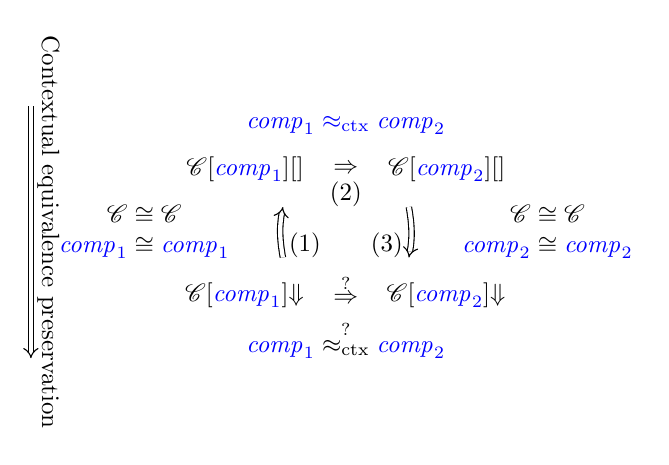
\begin{tikzpicture}[scale=0.8,every node/.style={scale=.9}]
    % \draw[help lines,yellow] (0,0) grid (10,7);
    \node at (5,4.7) { ${\src{\comp_1}\mathrel{\sconeq} \src{\comp_2}}$ };

    \node at (3.4,4) { ${\plug{\trg{\context}}{\src{\comp_1}} \sterm[]{\gc}{}}$ };
    \node at (5,4) { $\mathrel{\Rightarrow}$ };
    \node at (6.6,4) { ${\plug{\trg{\context}}{\src{\comp_2}} \sterm[]{\gc}{}}$ };

    \node at (4.35,2.8) { (1) };
    \node at (5,3.6) { (2) };
    \node at (5.65,2.8) { (3) };

    \draw[out=100,in=260,double,-implies,double equal sign distance] (4,2.6) to (4,3.4);

    \draw[out=280,in=80,double,-implies,double equal sign distance] (6,3.4) to (6,2.6);

    \node[align=center] at (8.2,3) { $ {\trg{\context}} \cong \trg{\context}$ \\
      $ {\src{\comp_2}} \cong {\src{\comp_2}}$};
    \node[align=center] at (1.8,3) { $ {\trg{\context}} \cong \trg{\context}$ \\
      $ {\src{\comp_1}} \cong {\src{\comp_1}}$};
    % \node at (9,2.7) { $e  {\src{C_1}} \cong \src{C_1}} : tau$ };
    % \node at (8.7,3.3) { $ {\trg{\context}} \cong \trg{\context} :{\emptyset},tau \ra e,{\cdots}$ };
    % \node at (.8,3) { $e  {\src{C_1}} \cong {\src{C_1}} : tau$ };

    \node at (3.4,2) { ${\plug{\trg{\context}}{\src{\comp_1}} \term[]{}}$ };
    \node at (5,2.1) { $\overset{?}{\Rightarrow}$ };
    \node at (6.6,2) { ${\plug{\trg{\context}}{\src{\comp_2}} \term[]{}}$ };

    \node at (5,1.3) { ${\src{\comp_1}}\mathrel{\overset{?}{\tconeq}}{\src{\comp_2}}$ };

    \draw[out=-90,in=90,double,-implies,double equal sign distance] (0,5) to node[sloped, yshift =.7em]{\Small Contextual equivalence preservation} (0,1);
  \end{tikzpicture}
  \caption{Proving one direction of fully abstract compilation (contextual equivalence preservation).}
  \label{fig:fa-proof-sketch}
\end{figure}


% \subsection{Proof sketch}
% \label{subsec:proof-sketch}
% \begin{proof}[Proof of Theorem~\ref{thm:full-abstraction}]
  % \item Consider first the upward arrow.
  %   Assume $\src{\var{comp}_1} \tconeq \src{\var{comp}_2}$.

  %   Take a $\src{\context}$ such that $\vdash \src{\context}$, take $\src{\ta[,i]}
  %   = \src{\dom(\var{comp}_i.\mscode)}$, $\gsigrets_i = \var{comp}_i.\sigrets$ and
  %   $\gsigcloss_i = \var{comp}_i.\sigcloss$, $\gc_i = (\ta[,i],\stkb_i,\gsigrets_i,\gsigcloss_i)$ and we will prove that
  %   $\src{\plug{\context}{\var{comp}_1} \sterm{\gc_1}} \Leftrightarrow
  %   \src{\plug{\context}{\var{comp}_2} \sterm{\gc_2}}$.

  %   By symmetry, we can assume w.l.o.g. that $\src{\plug{\context}{\var{comp}_1} \sterm{\gc_1}}$ and prove that $\src{\plug{\context}{\var{comp}_2} \sterm{\gc_2}}$.
  %   Note that this implies that $\src{\context}$ is a valid context for both $\src{\var{comp}_1}$ and $\src{\var{comp}_2}$.

  %   First, we show that also $\plug{\context}{\var{comp}_1} \trg{\term}$.
  %   Take $n$ the amount of steps in the termination of $\src{\plug{\context}{\var{comp}_1} \sterm{\gc_1}}$.
  %   It follows from Lemma~\ref{lem:ftlr-comps} that $\npair[n+1]{(\var{comp}_1,\var{comp}_1)} \in \lrcomp[\preceq,\gc_1](W_1)$ for some $W_1$ with $\dom(\pwfree) = \dom(\pwpriv) = \emptyset$.
  %   It also follows from the same Lemma~\ref{lem:ftlr-comps} that $\npair[n+1]{(\context,\context)} \in \lrcomp[\preceq,\gc_1](W_1')$ for some $W_1'$ that we can choose such that $W_1 \uplus W_1'$ is defined.
  %   Lemma~\ref{lem:compat-context-plug} then tells us that $\npair{(\plug{\context}{\var{comp}_1}, \plug{\context}{\var{comp}_1})} \in \lrec[\preceq,\gc_1](W_1\uplus W_1')$
  %   Together with $\src{\plug{\context}{\var{comp}_1} \sterm[n]{\gc_1}}$, Lemma~\ref{lem:adequacy} then tells us that $\plug{\context}{\var{comp}_1} \trg{\term}$.

  %   It follows from $\src{\var{comp}_1} \tconeq \src{\var{comp}_2}$ that also $\plug{\context}{\var{comp}_2} \trg{\term}$.

  %   It now remains to show that also $\src{\plug{\context}{\var{comp}_2} \sterm{\gc_2}}$.
  %   Take $n'$ the amount of steps in the termination of $\plug{\context}{\var{comp}_2} \trg{\term}$.
  %   It follows from Lemma~\ref{lem:ftlr-comps} that $\npair[n'+1]{(\var{comp}_2,\var{comp}_2)} \in \lrcomp[\succeq,\gc_2](W_2)$ for some $W_2$ with $\dom(\pwfree) = \dom(\pwpriv) = \emptyset$.
  %   It also follows from the same Lemma~\ref{lem:ftlr-comps} that $\npair[n'+1]{(\context,\context)} \in \lrcomp[\succeq,\gc_2](W_2')$ for some $W_2'$ that we can choose such that $W_2 \uplus W_2'$ is defined.
  %   Lemma~\ref{lem:compat-context-plug} then tells us that $\npair[n']{(\plug{\context}{\var{comp}_2}, \plug{\context}{\var{comp}_2})} \in \lrec[\succeq,\gc_2](W_2\uplus W_2')$
  %   Together with $\plug{\context}{\var{comp}_2} \trg{\term[n']}$, Lemma~\ref{lem:adequacy} then tells us that $\src{\plug{\context}{\var{comp}_2} \sterm{\gc_2}}$, concluding this direction of the proof.

%   First consider the right arrow:

%     Assume $\src{\var{comp}_1} \sconeq \src{\var{comp}_2}$. Take $\src{\ta[,i]} = \src{\dom(\var{comp}_i.\mscode)}$, $\gsigrets_i = \var{comp}_i.\sigrets$ and $\gsigcloss_i = \var{comp}_i.\sigcloss$, $\gc_i = (\ta[,i],\stkb_i,\gsigrets_i,\gsigcloss_i)$.
% %
%     Take a $\trg{\context}$ such that $\vdash \trg{\context}$ and we will prove that
%     $\trg{\plug{\context}{\var{comp}_1} \term} \Leftrightarrow
%     \trg{\plug{\context}{\var{comp}_2} \term}$.
% %
%     By symmetry, we can assume w.l.o.g. that $\trg{\plug{\context}{\var{comp}_1} \term}$ and prove that $\trg{\plug{\context}{\var{comp}_2} \term}$.
%     Note that this implies that $\trg{\context}$ is a valid context for both $\trg{\var{comp}_1}$ and $\trg{\var{comp}_2}$.
% %
%     First, we show that also $\plug{\context}{\var{comp}_1} \src{\sterm{\gc_1}}$.
%     Take $n$ the amount of steps in the termination of $\plug{\context}{\var{comp}_1} \trg{\term}$.
%     It follows from Lemma~\ref{lem:ftlr-comps} that $\npair[n+1]{(\var{comp}_1,\var{comp}_1)} \in \lrcomp[\succeq,\gc_1](W_1)$ for some $W_1$ with $\dom(\pwfree) = \dom(\pwpriv) = \emptyset$.
%     It also follows from the same Lemma~\ref{lem:ftlr-comps} that $\npair[n+1]{(\context,\context)} \in \lrcomp[\succeq,\gc_1](W_1')$ for some $W_1'$ that we can choose such that $W_1 \uplus W_1'$ is defined.
%     Lemma~\ref{lem:compat-context-plug} then tells us that $\npair{(\plug{\context}{\var{comp}_1}, \plug{\context}{\var{comp}_1})} \in \lrec[\succeq,\gc_1](W_1\uplus W_1')$
%     Together with $\plug{\context}{\var{comp}_1} \trg{\term[n]}$, Lemma~\ref{lem:adequacy} then tells us that $\plug{\context}{\var{comp}_1} \src{\sterm{\gc_1}}$.
% %
%     It follows from $\src{\var{comp}_1} \sconeq \src{\var{comp}_2}$ that also $\plug{\context}{\var{comp}_2} \src{\sterm{\gc_2}}$.
% %
%     It now remains to show that also $\plug{\context}{\var{comp}_2} \trg{\term}$.
%     Take $n'$ the amount of steps in the termination of $\plug{\context}{\var{comp}_2} \src{\sterm{\gc_2}}$.
%     It follows from Lemma~\ref{lem:ftlr-comps} that $\npair[n'+1]{(\var{comp}_2,\var{comp}_2)} \in \lrcomp[\preceq,\gc_2](W_2)$ for some $W_2$ with $\dom(\pwfree) = \dom(\pwpriv) = \emptyset$.
%     It also follows from the same Lemma~\ref{lem:ftlr-comps} that $\npair[n'+1]{(\context,\context)} \in \lrcomp[\preceq,\gc_2](W_2')$ for some $W_2'$ that we can choose such that $W_2 \uplus W_2'$ is defined.
%     Lemma~\ref{lem:compat-context-plug} then tells us that $\npair[n']{(\plug{\context}{\var{comp}_2}, \plug{\context}{\var{comp}_2})} \in \lrec[\preceq,\gc_2](W_2\uplus W_2')$
%     Together with $\plug{\context}{\var{comp}_2} \trg{\term[n']}$, Lemma~\ref{lem:adequacy} then tells us that $\plug{\context}{\var{comp}_2} \trg{\term}$, concluding the second direction of the proof.

%  The left arrow is proven in a similar manner.
% \end{proof}

%%% Local Variables:
%%% TeX-master: "paper"
%%% End:

\section{Discussion}
\label{sec:discussion}
% \begin{itemize}
% \item explain how fully abstract overlay semantics could form one pass of a verified secure compiler.
% \item Sharing stack references accross component boundaries is supported
% \item Other notions of well-bracketedness (specifically one would be to allow different stacks)
% \end{itemize}
\subsection{Full Abstraction}
% - Full abstraction proofs difficult
Our formulation of WBCF and LSE using a fully abstract overlay semantics has an important advantage with respect to others.
Imagine that you are implementing a fully abstract compiler for a high-level language, i.e.\ a secure compiler that enforces high-level abstractions when interacting with untrusted target-language components.
Such a compiler would need to perform many things and enforce other high-level properties than just WBCF and LSE.

If such a compiler uses the \stktokens{} calling convention, then the security proof should not have to reprove security of \stktokens{}.
Ideally, it should just combine security proofs for the compiler's other functionality with our results about \stktokens{}.
We point out that our formulation enables such reuse.
Specifically, the compiler could be factored into a part that targets \srccm{}, followed by our embedding into \trgcm{}.
If the authors of the secure compiler can prove full abstraction of the first part (relying on WBCF and LSE in \srccm{}) and they can also prove that this first part generates well-formed and reasonable components, then full abstraction of the whole compiler follows by our result and transitivity of fully abstract compilation.
Perhaps other reusable components of secure compilers could be formulated similarly using some form of fully abstract overlay semantics, to obtain similar reusability of their security proofs.

% When creating fully-abstract compilers between low-level machines, it is a big challenge to work with the exposed addresses.
% In particular, if the compilation changes the code size of a block of code, then it may be observable and prevent full-abstraction from being proven.
% We would argue that when a compilation reaches a phase where addresses are exposed, then the compilation should no longer change the code.
% This does, however, pose the challenge that there might quite a few abstractions in difference between the language where addresses are hidden to a machine where they are not.
% We propose that this challenge is solved by implementing these abstractions in a number of overlay semantics.
% By implementing them one by one, one can deal with one abstraction at a time reducing the complexity of each necessary full-abstraction proof.


% - Need to compile to a machine with enforcement mechanisms - capability machine an option
% - Full abstraction proofs modular, so other full abstraction proofs could target \srccm{} and thus have more abstractions to work with than if \trgcm{} was the target.

%\subsection{Sharing the stack}
% ?

\begin{jversion}
  A compiler is secure when it enforces the properties of high-level languages which begs the question what properties should we enforce.
  When it comes to fully-abstract compilation, then the answer is that all the properties of the high-level language should be enforced, so the real question is what high-level language we would like.
  \stktokens{} ensures a standard call-return control-flow, but if we want a different kind of control-flow, for instance call/CC, then we need to come up with a different enforcement scheme.
  Further, many high-level languages have exceptions which is yet another form of control-flow which is also not supported by \stktokens{}.
  This goes to show how we must consider what high-level language we want in order to answer the question of what properties we must enforce to get a fully-abstract compiler.
  % Lau: Say something about address hiding?

  We conjecture that \stktokens{} can support a limited form of continuations and exceptions.
  Specifically, the continuations and exceptions would be passed to the callee as sealed code capabilities.
  In order for the continuations and exceptions to work with the stack, they would have to be sealed with the return seals.
  \DDin{I'm not convinced that these limitations cannot be avoided. Perhaps we should keep this discussion more tentative?}
  This requirement puts two strong limitations on continuations and exceptions.
  First of all, they can be used by the immediate callee, but they cannot be used in subsequent calls made by the callee (assuming they use \stktokens{}).
  The problem is that the callee would have to take up part of the stack for their local stack frame.
  This would break up the return token that should be used with the continuation (or exception).
  If the callee really needs to pass on the continuation, then they would have to construct a wrapper that unravels the stack and restores the necessary return token.
  Second, a call that passes continuations or exceptions in this way has to pass the same continuations and exceptions in every call.
  The problem is that just like the return code capability, the continuation and exception capabilities are non-linear.
  This means that a callee can store them for subsequent calls preventing us from using different continuations and exceptions for different calls.

  \dominique{Also: should we mention the limited additional control flow we seem to get if we omit the stack base check (where  adversaries can use a kind of non-preemptive multi-threading)?}

\begin{thesisonly}
  % Say something about horizontal vs vertical composition.
  Fully-abstract compilers compose vertically which means that if we defined a compiler phase that targets \srccm{}, then we could use the full-abstraction theorem immediately.
  However, fully-abstract compilers do not extend horizontally in the sense that if we add a new feature in the target and source language, then the full-abstraction theorem does not follow immediately.
  Intuitively, this is the case because the new feature may have an unforeseen interaction with existing features that breaks a desired property.
  In order to enforce more language properties on capability machines, it is reasonable to assume that new capability primitives may be necessary.
  \stktokens{}, for instance, requires linear capabilities, and \citet{skorstengaard_reasoning_2017} uses local capabilities to enforce WBCF and LSE.
  In order to implement address-hiding (i.e.\ have references that do not expose the address they actually point to), it is reasonable to believe that one would need a new capability primitive.
  After all, the capabilities we use here do not hide the addresses in any meaningful way, so a new ``address hiding'' capability would be necessary to enforce this property.
  If we extended \trgcm{} and \srccm{} with such new capabilities, then we would have to redo the entire full-abstraction proof.
\end{thesisonly}

  % new paragraph: conditional full-abstraction
  \dominique{This paragraph should perhaps also point out the link to the dynamic compromise paper?}
  Our full-abstraction theorem, Theorem~\ref{thm:full-abstraction}, is not pure full-abstraction as it requires the components to be reasonable and well-formed.
  In other words, if we were to define a compiler phase that targets \srccm{}, then we would also have to show that every program it generates is well-formed and reasonable in order to use the full-abstraction result.
  Without the reasonability constraint, \stktokens{} would have to enforce reasonability instead.
  That is, \stktokens{} would have to dynamically ensure that no return seals or means to get return seals are passed in calls.
  Essentially, such checks would protect the trusted code against itself which shouldn't be necessary in the first place.
  Instead, the compiler should generate reasonable code that never exhibits the unreasonable behaviour.
  This should be done in a compiler phase where more information about the original program is available, e.g.\ the compilation phase that commits to the low-level translation.
  Similarly for the syntactic constraints given by well-formedness.
  The compiler should make sure to generate code that satisfies the well-formedness judgement, so it can be executed by the machine.

  % TODO new paragraph: Machine checked proof. MANY details, any future work should be machine checked?
  One challenge in full-abstraction proofs is to relate the translation of program to the program it was translated from.
  Such a relation is often expressed as a back-translation  \citep{devriese_modular_2017}, i.e.\ a translation from the target language to the source language.
  When we use an overlay semantics, the back-translation becomes trivial because the source and target language are syntactically the same, so the identity can be used as the back-translation.
  If we have native call and return instructions in the source language, then the source language would be different from the target language, and we would have to use a non-trivial back-translation.
  Specifically, the back-translation would need to distinguish sequences of instructions that is the translation of a call from sequences of instructions that just look like a call.
  With overlay semantics, this is not a concern because everything that looks like a call is interpreted as a call.
\end{jversion}

\subsection{Practical Applicability}
We believe there are good arguments for practical applicability of \stktokens{}.
The strong security guarantees are proven in a way that is reusable as part of a bigger proof of compiler security.
Its costs are
\begin{itemize}
\item a constant and limited amount of checks on every boundary crossing.
\item possibly a small memory overhead because stack frames must be of non-zero length
\end{itemize}
The main caveat is that we rely on the assumption that capability machines like CHERI can be extended with linear capabilities in an efficient way.

Although this assumption can only be discharged by demonstrating an actual implementation with efficiency measurements, the following notes are based on private discussions with people from the CHERI team as well as our own thoughts on the matter.
As we understand it, the main problems to solve for adding linear capabilities to a capability machine like CHERI are related to the move semantics for instructions like \texttt{move}, \texttt{store} and \texttt{load}.
Processor optimizations like pipelining and out-of-order execution rely on being able to accurately predict the registers and memory that an instruction will write to and read from.
Our instructions are a bit clumsy from this point-of-view because, for example, \texttt{move} or \texttt{store} will zero the source register resp. memory location if the value being written is linear.
A solution for this problem could be to add separate instructions for moving, storing and loading linear registers at the cost of additional opcode space.
Adding splice and split will also consume some opcode space.

Another problem is caused by the move semantics for \texttt{load} in the presence of multiple hardware threads.
In this setting, zeroing out the source memory location must happen atomically to avoid race conditions where two hardware threads end up reading the same linear capability to their registers.
This means that a \texttt{load} of a linear capability should behave atomically, similar to a primitive compare-and-swap instruction.
This is in principle not a problem except that atomic instructions are significantly slower than a regular \texttt{load} (on the order of 10x slower or more).
When using \stktokens{}, loads of linear capabilities happen only when a thread has stored its return data capability on the stack and loads it back from there after a return.
Because the stack is a region of memory with very high thread affinity (no other hardware thread should access it, in principle), and which is accessed quite often, well-engineered caching could perhaps reduce the high overhead of atomic loads of linear capabilities.
% If such memory could be (mostly) kept exclusively locked in a cache close to the processor, the overhead of atomic loads in \stktokens{} might be significantly less than \texttt{load}'s worst case.
The processor could perhaps also (be told to) rely on the fact that race conditions should be impossible for loads from linear capabilities (which should in principle be non-aliased) and just use a non-atomic load in that case.

\begin{jversion}
Programs that use a C-like calling convention often allow programs to pass a stack reference in a call either to provide a reference for a piece of memory to work on or to indicate where the result of the call should be placed.
\stktokens{} does not support this as it expects to get a stack pointer for the entire stack it handed out.
\dominique{Err... I don't see the problem.
  Passing stack references to callees should work fine, as long as the callee treats them linearly (i.e.\ doesn't try to copy them).
  }
However, if we have allocated part of the stack for a different purpose and handed out a reference for it, then the stack pointer cannot reference the same memory as the stack pointer is a linear capability.
\dominique{I don't understand this sentence.}
However, while it is not possible to allocate a reference for the stack, one can easily imagine that the stack could still be used to pass and return values.
\dominique{Or this one...}
\end{jversion}

\dominique{Perhaps worth mentioning the problem with adding support for linear values in a real C compiler: how to explain to the compiler that it should treat the linear values linearly and not use optimizations that will break this.}

%%% Local Variables:
%%% TeX-master: "paper"
%%% End:

\section{Related Work}
\label{sec:related-work}
In this section, we discuss related work on securely enforcing control flow correctness and/or local state encapsulation or the linear capabilities we use to do it.
We do not repeat the work we discussed in Section~\ref{sec:introduction}.

Capability machines originate with \citet{dennis_programming_1966} and we refer to \citet{levy_capability-based_1984} and \citet{watson_cheri_2015} for an overview of previous work.
The capability machine formalized in Section~\ref{sec:cap-mach-w-seal-and-lin} is modelled after CHERI~\citep{watson_cheri_2015,woodruff_cheri_2014}.
This is a recent, relatively mature capability machine which combines capabilities with a virtual memory approach in the interest of backwards compatibility and gradual adoption.
For simplicity, we have omitted features of CHERI that were not needed for \stktokens{} (e.g.\ local capabilities, virtual memory).

Plenty of other papers enforce well-bracketed control flow at a low level but most are restricted to preventing particular types of attacks and enforce only partial correctness of control flow.
This includes particularly the line of work on control-flow integrity~\citep{abadi_control-flow_2005}.
This technique prevents certain classes of attacks by sanitizing addresses before direct and indirect jumps based on static control graph information and a protected shadow stack.
Contrary to \stktokens{}, CFI can be implemented on commodity hardware rather than capability machines.
However, its attacker model is different, and its security goals are weaker.
They assume an attacker that is unable to execute code but can overwrite arbitrary data at any time during execution (to model buffer overflows).
In terms of security goals, the technique does not enforce local stack encapsulation.
Also, it only enforces a weak form of control flow correctness saying that jumps stay within the program's static control flow graph~\citep{Abadi2005Theory}.
Such a property ignores temporal properties and seems hard to use for reasoning.
There is also more and more evidence that these partial security properties are not enough to prevent realistic attacks in practice~\citep{Evans:2015:CJW:2810103.2813646,Carlini2015ControlFlowBending,van_der_veen_dynamics_2017}.

More closely related to our work are papers that use separate per-component stacks, a trusted stack manager and some form of memory isolation to enforce control-flow correctness as part of a secure compilation result~\citep{patrignani_modular_2016,juglaret_beyond_2016}.
Our work differs from theirs in that we use a different low-level security primitive (a capability machine with local capabilities rather than a machine with a primitive notion of compartments), and we do not use per-component stacks or a trusted stack manager but a single shared stack and a decentralized calling convention based on linear capabilities.
Both prove a secure compilation result from a high-level language which clearly implies a general form of control-flow correctness, but that result is not separated from the results about other aspects of their compiler.

CheriBSD applies a similar approach with separate per-component stacks and a trusted stack manager on a capability machine~\citep{watson_cheri_2015}.
The authors use local capabilities to prevent components from accidentally leaking their stack pointer to other components, but there is no actual capability revocation in play.
They do not provide many details on this mechanism and it is, for example, not clear if and how they intend to deal with higher-order interfaces (C function pointers) or stack references shared across component boundaries. 

The fact that our full abstraction result only applies to reasonable components (see Section~\ref{sec:form-secur-with}) makes it related to full abstraction results for unsafe languages.
In their study of compartmentalization primitives, \Citet{juglaret_beyond_2016} discuss the property of Secure Compartmentalizing Compilation (SCC): a variant of full abstraction that applies to unsafe source languages.
Essentially, they modify standard full abstraction so that preservation and reflection of contextual equivalence are only guaranteed for components that are {\itshape fully defined}, which means essentially that they do not exhibit undefined behavior in any fully defined context.
If we see reasonable behavior as defined behavior, then our full abstraction result can be seen as an application of this same idea.

In follow-up work, \citet{Abate:2018:GCG:3243734.3243745} extend this approach to components with  undefined behavior by proving secure compilation guarantees for the execution until the undefined behavior happens. 
Another interesting relation between our work and that of \citet{Abate:2018:GCG:3243734.3243745}, is that they consider dynamic compromise scenarios, where some components start out as trusted until they are compromised and are treated as adversarial after that.
Our full abstraction result does not apply to those scenarios because it is intended to be used in the verification of a secure compiler where such scenarios are not relevant.
Nevertheless, we believe our Fundamental Theorem of Logical Relations (see Section~\ref{thm:ftlr}) does apply in such scenarios because it is step-bounded.
To deal with the evolving classification of components as trusted or adversarial, we can simply apply the theorem several times with different choices of $\ta$ and taking $n$ small enough that the compromise of $\ta$ has not yet happened until that point. 
Because the theorem only requires reasonability up to $n$ steps, we get well-bracketedness guarantees up to the right step in the execution.
This can be seen as a step-bounded version of the idea explained in \citep{patrignani_modular_2016}.
It is an interesting observation that modular secure compilation, combined with step-bounded reasoning is sufficient to cover dynamic compromise scenarios without the need to build in dynamic compromise scenarios into the definition of secure compilation like \citet{Abate:2018:GCG:3243734.3243745}.

Local capabilities can be used to ensure well-bracketed control-flow and local-state encapsulation as demonstrated by \citet{skorstengaard_reasoning_2017}.
Recently, \citet{tsampas_2019} demonstrated that an extension of local capabilities with multiple linearly ordered colours can be used to enforce the life time of stack references.
Specifically, a stack reference should not be able to outlive the stack frame it points to.
If \stktokens{} was extended with stack references, then it would also enforce reference life times.
Specifically in order to return from a call, we must use the return token, i.e.\ the stack.
The stack is linear, so if there are references to it, aside from the stack capability itself, then we cannot have a complete return token.
This means that we have to splice all the stack references together with the stack capability to complete the return token in order to return.
\citet{tsampas_2019} allow (almost) normal references that can be stored in multiple places at the same time.
This means that their approach is more like C than \stktokens{}.
As explained in Section~\ref{sec:introduction}, these approaches have the downside that they require stack clearing (including unused parts) on boundary crossings.

In addition to the already-mentioned work on linear capabilities, \citet{van_strydonck_linear_2019} have recently used them in a secure (fully abstract) compiler for a C-like language with separation logic contracts.
A form of linear capabilities was also used in the SAFE machine developed within the CRASH/SAFE project \citep{DBLP:conf/sp/AmorimDGHPST15,DBLP:journals/jcs/AmorimCDDHPPPT16}.
\citet{Abate:2018:GCG:3243734.3243745} used micro-policy enforced linear return capabilities to ensure a cross-component stack discipline.
Their linear capabilities were designed specifically to enforce the stack discipline but behave similarly to ours with the notable difference that their linear return pointers are destroyed in a jump.

There are other notions of secure compilation than full-abstraction~\citep{abadi_protection_1998}.
\citet{abate_2019} present an overview of trace-based secure compilation properties.
Full abstraction is only one, relatively weak, property in their hierarchy.
It would be interesting to investigate if our compiler, i.e.\ the embedding function from \srccm{} into \trgcm{}, also satisfies some of their other properties.
While our current result implies that we can prove contextual equivalences in \trgcm{} components using \stktokens{}, by proving them instead in the more well-behaved \srccm{} semantics, such stronger properties would imply that we can also prove robust preservation of other (hyper-)properties in a similar manner.
As our back-translation works for arbitrary programs, we expect that, in addition to full abstraction, our embedding also satisfies Robust Relational Hyperproperty Preservation (RrHP, the strongest property in the hierarchy of \citeauthor{abate_2019}) and that a large part of our current proof (the back-translation and the logical relation) could be reused to establish this.
However, to do this, we would first need to extend our semantics with some form of traces and we have not investigated how best to do this. 


% \begin{acks}                            %% acks environment is optional
%                                         %% contents suppressed with 'anonymous'
%   %% Commands \grantsponsor{<sponsorID>}{<name>}{<url>} and
%   %% \grantnum[<url>]{<sponsorID>}{<number>} should be used to
%   %% acknowledge financial support and will be used by metadata
%   %% extraction tools.
%   This material is based upon work supported by the
%   \grantsponsor{GS100000001}{National Science
%     Foundation}{http://dx.doi.org/10.13039/100000001} under Grant
%   No.~\grantnum{GS100000001}{nnnnnnn} and Grant
%   No.~\grantnum{GS100000001}{mmmmmmm}.  Any opinions, findings, and
%   conclusions or recommendations expressed in this material are those
%   of the author and do not necessarily reflect the views of the
%   National Science Foundation.
% \end{acks}

\section*{Acknowledgements}
  This research was supported in part by the ModuRes Sapere Aude Advanced Grant
  from The Danish Council for Independent Research for the Natural Sciences (FNU).
  Support for an STSM was received from COST Action EUTypes (CA15123).
  Dominique Devriese held a Postdoctoral fellowship from the Research Foundation
  Flanders (FWO) during most of this research.
  This research was supported in part by the Research Foundation Flanders (FWO).
  Conflicts of Interest: None.

\bibliography{references}



\clearpage
\appendix
\section{\trgcm{} instruction interpretation}
\label{app:instr-interpretation}
In this section, we present the interpretation of the \trgcm{} instructions left out of \figurename~\ref{fig:target-op-sem} as well as the interpretation of the \srccm{} specific interpretation.
The two interpretations have everything in black in common, and everything in blue is specific to \srccm{}.

 \begin{tabular}{|>{$}c<{$}|>{$}p{3.7cm}<{$}|>{\raggedright\arraybackslash}p{6.2cm}|}
    \hline
    i \in \Instr                                 & \sem{i}(\Phi) & Conditions\\
    \hline
    \tgetb{r_1}{r_2}                                        & \updPcAddr{\Phi\updReg{r_1}{w}} & If $\Phi(r_2) = ((\_,\_),\baddr,\_,\_)$, $\Phi(r_2) = \seal{\baddr,\_,\_}$, \src{or $\Phi(r_2) = ((\_,\_),\baddr,\_,\_)$}, then $w = \baddr$ and otherwise $w = -1$\\
    \hline
    \tgete{r_1}{r_2}                                        & \updPcAddr{\Phi\updReg{r_1}{w}} & If $\Phi(r_2) = ((\_,\_),\_,\eaddr,\_)$, or $\Phi(r_2) = \seal{\_,\eaddr,\_}$, \src{or $\Phi(r_2) = ((\_,\_),\_,\eaddr,\_)$}, then $w = \eaddr$ and otherwise $w = -1$\\
    \hline
    \tisptr{r_1}{r_2} & \updPcAddr{\Phi\updReg{r_1}{w}} & $w = \encType{\Phi(r_2)}$\footnote{The $\encType$ function differs for the two machines. Depending on the machine, the appropriate function is used.}\\
    \hline
    \tgetlin{r_1}{r_2} &\updPcAddr{\Phi\updReg{r_1}{w}} & If $\isLinear{\Phi(r_2)}$, then $w = \encLin{\linear}$, otherwise $w= \encLin{\normal}$\\
    \hline
    \tgetp{r_1}{r_2} & \updPcAddr{\Phi\updReg{r_1}{w}} & If $\Phi(r_2) = ((\perm,\_),\_,\_,\_)$ \src{or $\Phi(r_2) = ((\perm,\_),\_,\_,\_)$}, then $w = \encPerm{\perm}$ and otherwise $w = -1$\\
    \hline
    \tjnz{r}{\rn} & \Phi\updReg{r}{w}\update{\pcreg}{\Phi(r)} & $\nonZero{\Phi(\rn)}$ and $w = \linCons{\Phi(r)}$\\
    \hline
    \tjnz{r}{\rn} & \updPcAddr{\Phi}& If not $\nonZero{\Phi(\rn)}$ \\
    \hline
    \tplus{r}{\rn_1}{\rn_2} & \updPcAddr{\Phi\updReg{r}{n_1+n_2}} & If for $i \in \{1,2\}$ $\Phi(\rn_i) = n_i \in \ints$ \\
    \hline
    \tminus{r}{\rn_1}{\rn_2} & \updPcAddr{\Phi\updReg{r}{n_1-n_2}} & If for $i \in \{1,2\}$ $\Phi(\rn_i) = n_i \in \ints$ \\
    \hline
    \tlt{r}{\rn_1}{\rn_2} & \updPcAddr{\Phi\updReg{r}{1}} & If for $i \in \{1,2\}$ $\Phi(\rn_i) = n_i \in \ints$ and $n_1 < n_2$ \\
    \hline
    \tlt{r}{\rn_1}{\rn_2} & \updPcAddr{\Phi\updReg{r}{0}} & If for $i \in \{1,2\}$ $\Phi(\rn_i) = n_i \in \ints$ and $n_1 \not< n_2$ \\
    \hline
    \tsetatob{r} & \updPcAddr{\Phi\updReg{r}{c}} & $r \neq \pcreg$, $\Phi(r) = ((\perm,\lin),\baddr,\eaddr,\_)$, and $c = ((\perm,\lin),\baddr,\eaddr,\baddr)$ \\
    \hline
    \tsetatob{r} & \updPcAddr{\Phi\updReg{r}{c}} & $r \neq \pcreg$, $\Phi(r) = \seal{\sigma_\baddr,\sigma_\eaddr,\_}$, and $c = \seal{\sigma_\baddr,\sigma_\eaddr,\sigma_\baddr}$ \\
    \hline
    \src{\texttt{seta2b}\; r} & \src{\updPcAddr{\Phi\updReg{r}{c}}} &\srcalt{$r \neq \pcreg$, $\Phi(r) = \stkptr{\perm,\baddr,\eaddr,\_}$, and $c = \stkptr{\perm,\baddr,\eaddr,\baddr}$} \\
    \hline
    \trestrict{r}{\rn} & \updPcAddr{\Phi\updReg{r}{c}} & If $\Phi(r) = ((\perm,\lin),\baddr, \eaddr,\aaddr)$ and $\Phi(\rn) = n$ and $\decPerm{n} \le \perm$ and $c = ((\decPerm{n},\lin),\baddr, \eaddr, \aaddr)$\\
    \hline
    \src{\texttt{restrict} \; r \; \rn} & \src{\updPcAddr{\Phi\updReg{r}{c}}} & \srcalt{If $\Phi(r) = \stkptr{\perm,\baddr, \eaddr,\aaddr}$ and $\Phi(\rn) = n$ and $\decPerm{n} \le \perm$ and $c = \stkptr{\decPerm{n},lin),\baddr, \eaddr, \aaddr}$}\\
    \hline
  \end{tabular}

Where $\nonZero{}$ is defined as follows
\[
  \nonZero{w} \defeq
  \begin{cases}
    \bot & w \in \ints \tand w = 0 \\
    \top & \totherwise
  \end{cases}
\]

  
%%% Local Variables:
%%% TeX-master: "paper"
%%% End:

\label{lastpage01}
\end{document}
 